\section{One Byte, Two Byte Exceptions}
\label{sec:vbbe21}
%\begin{figure}
%\centering
	\begin{tikzpicture}[node distance=0cm,start chain=1 going right] \footnotesize
  \tikzstyle{mytape}=[draw,minimum height=1.5cm]
	\node(A1)  [on chain=1,mytape,fill=blue!20] {$\underset{\text{exceptions}}{\underbrace{\overbracket{\text{ }e\text{ }}^{\text{2 bytes}}}_{\text{number of}}}$};
	\node(A2)  [on chain=1,mytape,fill=yellow!20] {$\underbrace{\overbracket{p_1,p_2,\dots,p_e}^{4e\text{ bytes}}}_{\text{exception positions}}$};
	\node(A3)  [on chain=1,mytape,fill=yellow!35] {$\underbrace{\overbracket{x_{p_1},x_{p_2},\dots,x_{p_e}}^{2e\text{ bytes}}}_{\text{two byte exceptions}}$};
	\node(A4)  [on chain=1,mytape,fill=green!35] {$\underbrace{\overbracket{x_{q_1},x_{q_2},\dots,x_{q_{n-e}}}^{n-e\text{ bytes}}}_{\text{one byte data}}$};
\end{tikzpicture}
%	\caption[The vbe21 encoding.]{\label{fig:vbe21} The vbe21 encoding takes two byte integers
%	$x_1,x_2,\dots,x_n$ and encodes those which cannot fit into one byte as
%	\textit{exceptions} at the beginning of the stream. There are $e$
%	exceptions which are recorded by their original positions
%	$p_1,p_2,\dots,p_e$ and values $x_{p_1},x_{p_2},\dots,x_{p_e}$.
%	Following this is the regular one byte data where $q_i$ is the original
%	position of the $i$-th one byte data point. This is beneficial when
%	there are few exceptions in the data.}
%\end{figure}


The one byte, two byte exceptions encoding, abbreviated to \textit{vbe21},
encodes a list of integers using one byte for each integer except for integers
which cannot fit into one byte, known as \textit{exceptions}, which are encoded
using two bytes. See Figure \ref{fig:vbe21}. Rather than using a control code to
mark where normal data and exceptions occur as in the Stream VByte codec
(Section \ref{subsubsec:svb}), the exceptions are encoded at the beginning since
it is expected that exceptions will occur with small probability.

The number of exceptions is written using 2 bytes, followed by the exceptions'
positions in the list using 4 bytes each, the exceptions themselves using 2
bytes each and finally the regular one byte data. For example, consider the
sequence of integers $1024,12,10,4096,0,1,2,1024$. There are three
exceptions 1024, 4096 and 1024. Hence, vbe21 would use
\[ 2 + 3(4+2) + 8-3 = 25 \]
bytes for this sequence. See Figure \ref{fig:vbe21-eg}.

\begin{figure}
\centering\begin{tikzpicture}[node distance=0cm,start chain=1 going right,start chain=2 going right] \footnotesize
  \tikzstyle{mytape}=[draw,minimum height=1.4cm]
    \node(A1)  [on chain=1,mytape,fill=blue!20] {$\underbrace{\overbracket{\texttt{0x00}|\texttt{0x03}}^{\text{2 bytes}}}_{3}$};
    \node(A2)  [on chain=1,mytape,fill=yellow!20] {$\underbrace{\overbracket{\texttt{0x00}|\texttt{0x00}|\texttt{0x00}|\texttt{0x00}}^{\text{4 bytes}}}_{0}$};
    \node(A3)  [on chain=1,mytape,fill=yellow!20] {$\underbrace{\overbracket{\texttt{0x00}|\texttt{0x00}|\texttt{0x00}|\texttt{0x03}}^{\text{4 bytes}}}_{3}$};
    \node(A4)  [on chain=1,mytape,fill=yellow!20] {$\underbrace{\overbracket{\texttt{0x00}|\texttt{0x00}|\texttt{0x00}|\texttt{0x07}}^{\text{4 bytes}}}_{7}$};
    \node(B1)  [on chain=2,mytape,fill=yellow!35,below of=A1,node distance=1.4cm] {$\underbrace{\overbracket{\texttt{0x04}|\texttt{0x00}}^{\text{2 bytes}}}_{1024}$};
    \node(B2)  [on chain=2,mytape,fill=yellow!35] {$\underbrace{\overbracket{\texttt{0x10}|\texttt{0x00}}^{\text{2 bytes}}}_{\num{4096}}$};
    \node(B3)  [on chain=2,mytape,fill=yellow!35] {$\underbrace{\overbracket{\texttt{0x04}|\texttt{0x00}}^{\text{2 bytes}}}_{1024}$};
    \node(B4)  [on chain=2,mytape,fill=green!35] {$\underbrace{\overbracket{\texttt{0x0c}}^{\text{1 byte}}}_{12}$};
    \node(B5)  [on chain=2,mytape,fill=green!35] {$\underbrace{\overbracket{\texttt{0x0a}}^{\text{1 byte}}}_{10}$};
    \node(B6)  [on chain=2,mytape,fill=green!35] {$\underbrace{\overbracket{\texttt{0x00}}^{\text{1 byte}}}_{0}$};
    \node(B7)  [on chain=2,mytape,fill=green!35] {$\underbrace{\overbracket{\texttt{0x01}}^{\text{1 byte}}}_{1}$};
    \node(B8)  [on chain=2,mytape,fill=green!35] {$\underbrace{\overbracket{\texttt{0x02}}^{\text{1 byte}}}_{2}$};
\end{tikzpicture}

	\caption[An example of $1024,12,10,4096, 0,1,2,1024$ encoded with vbe21.]{\label{fig:vbe21-eg} An example of $1024,12,10,4096,
	0,1,2,1024$ encoded with vbe21. The encoding order is read from left to
	right and top to bottom. There are 3 exceptions located at positions 0,
	3 and 7 with values 1024, 4096 and 1024. It uses 25 bytes in total.}
\end{figure}


Now, consider applying encoding $A$ to a read. Let $C_A:\Omega\to\mathbb{N}_0$
be a random variable measuring the resulting compressed size in bytes where
$\Omega$ is the space of possible nanopore reads. Then
\begin{align*}
	C_{vbe21} &= \text{exceptions} + \text{one byte data}\\
	&= (2 + 6X) + (N - X)\\
	&= 2 + 5X + N
\end{align*}
where $N$ and $X$ are random variables measuring the read length and number of
exceptions respectively. Recall from Section \ref{subsec:prob} that the
probability that a zig-zag delta is greater than 255 and therefore outside the one
byte range is $\sim 5\times 10^{-5}$ for the data. Thus, the expected number of
zig-zag delta exceptions is
\[ E[X] = (5 \times 10^{-5})E[N] \]
%Also, the read lengths can be modelled by the Gamma distribution $\Gamma(1.0885,0.0096)$.
where the expected read length is
\[ E[N] = 113471.4 \]
from Table \ref{tab:n}. So $E[X] \approx 5.67$, that is we expect roughly 5 to 6
exceptions per read when using the zig-zag delta transformation.
Then, the expected compressed size is given by
\begin{align*}
	E[C_{vbe21-zd}] &= 2 + (2.5\times 10^{-4})E[N]+ E[N]\\
	&= 2 + 1.00025E[N]\\
	&\approx 113502 \text{ bytes}
\end{align*}
where vbe21-zd means first apply the zig-zag delta encoding then vbe21. In
comparison, using the Stream VByte 16 (or \textit{svb16}) encoding, the
compressed size is given by
\begin{align*}
	C_{svb16} &= \lceil N/8 \rceil + 2X + (N - X)\\
	&= \lceil N/8 \rceil + X + N.
\end{align*}
Then, the expected compressed size is
\begin{align*}
	E[C_{svb16-zd}] &= \lceil E[N]/8 \rceil + (5 \times 10^{-5})E[N] + E[N]\\
	&= \lceil E[N]/8 \rceil + 1.00005E[N]\\
	&\approx 127661 \text{ bytes}\\
	&> E[C_{vbe21-zd}].
\end{align*}

This translates into roughly 8 bits per data point for vbe21-zd versus
9 for svb16-zd.
%See Table \ref{tab:vbe21-bpp}.
Intuitively these numbers make sense considering vbe21-zd essentially represents
most points using one byte each and svb16-zd stores one extra bit per point in
the control byte section.  Compare this to the entropy of the data which is 7.70
bits per point or 5.39 for the zig-zag deltas. So it is clear that
vbe21-zd saves more space than svb16-zd: roughly 14 KiB on average per read or
an estimated 6.6 GiB for the whole data set. However, this is merely a container
for the data which is useful for downstream compression; alone it doesn't
provide great compression results as is obvious when comparing it to the entropy
of the data.

vbe21-zd is linear in time complexity during encoding since it requires
applying the zig-zag delta transformation and checking which values are
exceptions. The same is true for decoding and the svb16-zd codec.

%\begin{table}
    \caption{\label{tab:vbe21-bpp} The theoretical expected bits per point for the
vbe21-zd and svb16-zd encodings.}
    \begin{tabular}{|l|l|}
        \hline
Encoding & Expected Bits Per Point\\
        \hline
vbe21-zd & 8\\
svb16-zd & 9\\
	\hline
    \end{tabular}
\end{table}


\subsection{Exceptions Encoding}

There are better ways of storing the exceptions than in the raw sequential
format of vbe21.
As we have seen there are usually 5 to 6 exceptions per read meaning that
storing the number of exceptions using two bytes which has a range of 0 to 65535
for all reads is wasteful.
In particular, the number of exceptions per read ranges from 0 to 3616 but 99\%
of reads have between 0 and 42 exceptions. See Table \ref{tab:ex}. Its
distribution, shown in Figure \ref{fig:nex-hist}, could be nicely fitted by an
exponential distribution. In fact, around 20\% of the reads have no exceptions
at all.

\begin{table}
    \caption{\label{tab:ex} Summary statistics of the number of exceptions per read and the zig-zag delta exceptions themselves in the data.}
	\begin{tabular}{|l|m{1.8cm}|l|}
	    \hline
	    Statistic & Number of Exceptions Per Read & Exceptions\\
        \hline
		Min &0 & 256\\
		Q1 & 1& 260\\

		Q2 & 3& 266\\
		Q3 & 6& 278\\
		Max & 3616& 2317\\
\hline
		Mean & 4.8546&277.0465\\
		Mode & 0&256\\
		SD & 18.0595&36.8207\\
	\hline
    \end{tabular}
\end{table}

\begin{figure}
	\centering
% Created by tikzDevice version 0.12.3.1 on 2022-10-11 18:23:57
% !TEX encoding = UTF-8 Unicode
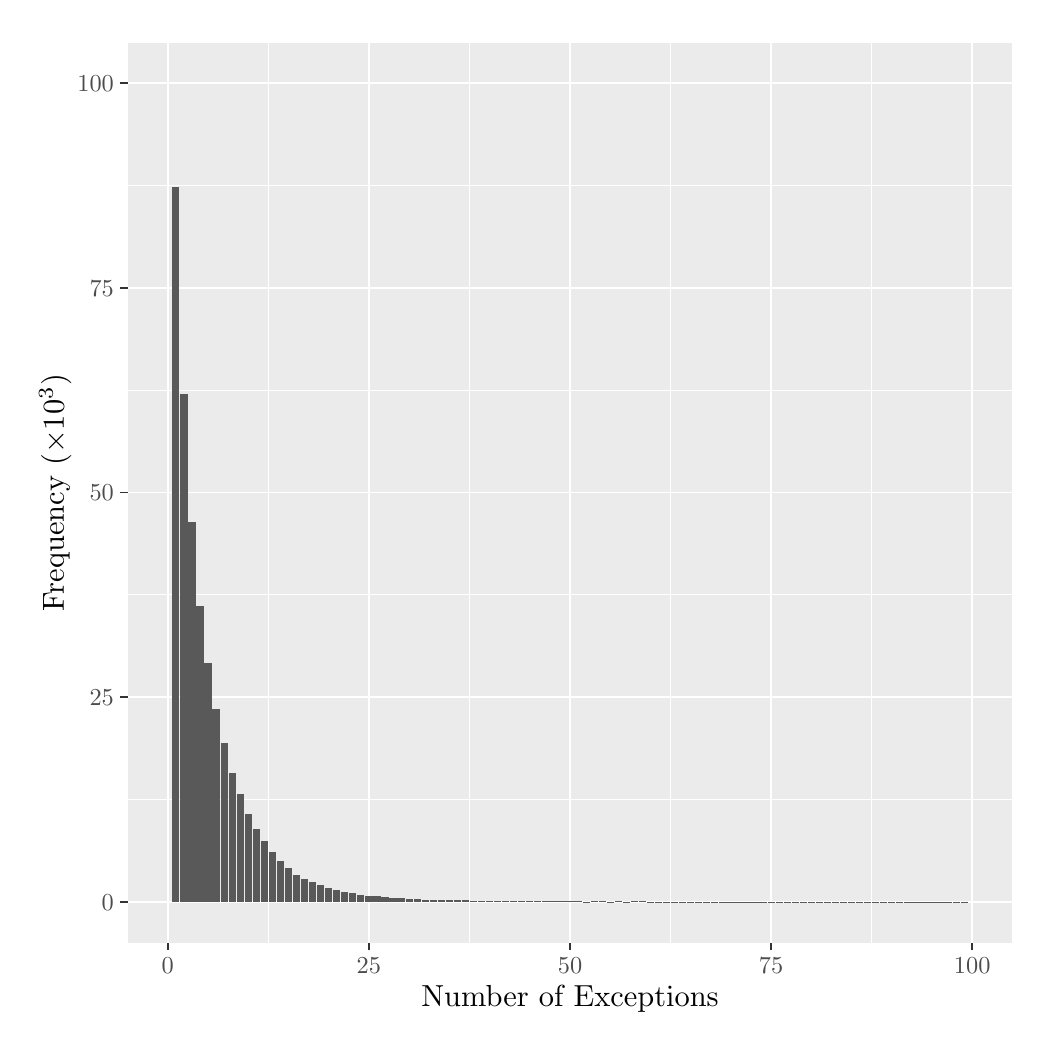
\begin{tikzpicture}[x=1pt,y=1pt]
\definecolor{fillColor}{RGB}{255,255,255}
\path[use as bounding box,fill=fillColor,fill opacity=0.00] (0,0) rectangle (361.35,361.35);
\begin{scope}
\path[clip] (  0.00,  0.00) rectangle (361.35,361.35);
\definecolor{drawColor}{RGB}{255,255,255}
\definecolor{fillColor}{RGB}{255,255,255}

\path[draw=drawColor,line width= 0.6pt,line join=round,line cap=round,fill=fillColor] (  0.00,  0.00) rectangle (361.35,361.35);
\end{scope}
\begin{scope}
\path[clip] ( 36.11, 30.69) rectangle (355.85,355.85);
\definecolor{fillColor}{gray}{0.92}

\path[fill=fillColor] ( 36.11, 30.69) rectangle (355.85,355.85);
\definecolor{drawColor}{RGB}{255,255,255}

\path[draw=drawColor,line width= 0.3pt,line join=round] ( 36.11, 82.45) --
	(355.85, 82.45);

\path[draw=drawColor,line width= 0.3pt,line join=round] ( 36.11,156.42) --
	(355.85,156.42);

\path[draw=drawColor,line width= 0.3pt,line join=round] ( 36.11,230.38) --
	(355.85,230.38);

\path[draw=drawColor,line width= 0.3pt,line join=round] ( 36.11,304.35) --
	(355.85,304.35);

\path[draw=drawColor,line width= 0.3pt,line join=round] ( 86.98, 30.69) --
	( 86.98,355.85);

\path[draw=drawColor,line width= 0.3pt,line join=round] (159.65, 30.69) --
	(159.65,355.85);

\path[draw=drawColor,line width= 0.3pt,line join=round] (232.31, 30.69) --
	(232.31,355.85);

\path[draw=drawColor,line width= 0.3pt,line join=round] (304.98, 30.69) --
	(304.98,355.85);

\path[draw=drawColor,line width= 0.6pt,line join=round] ( 36.11, 45.47) --
	(355.85, 45.47);

\path[draw=drawColor,line width= 0.6pt,line join=round] ( 36.11,119.43) --
	(355.85,119.43);

\path[draw=drawColor,line width= 0.6pt,line join=round] ( 36.11,193.40) --
	(355.85,193.40);

\path[draw=drawColor,line width= 0.6pt,line join=round] ( 36.11,267.37) --
	(355.85,267.37);

\path[draw=drawColor,line width= 0.6pt,line join=round] ( 36.11,341.34) --
	(355.85,341.34);

\path[draw=drawColor,line width= 0.6pt,line join=round] ( 50.64, 30.69) --
	( 50.64,355.85);

\path[draw=drawColor,line width= 0.6pt,line join=round] (123.31, 30.69) --
	(123.31,355.85);

\path[draw=drawColor,line width= 0.6pt,line join=round] (195.98, 30.69) --
	(195.98,355.85);

\path[draw=drawColor,line width= 0.6pt,line join=round] (268.65, 30.69) --
	(268.65,355.85);

\path[draw=drawColor,line width= 0.6pt,line join=round] (341.32, 30.69) --
	(341.32,355.85);
\definecolor{fillColor}{gray}{0.35}

\path[fill=fillColor] ( 52.24, 45.47) rectangle ( 54.86,303.76);

\path[fill=fillColor] ( 55.15, 45.47) rectangle ( 57.77,229.02);

\path[fill=fillColor] ( 58.06, 45.47) rectangle ( 60.67,182.55);

\path[fill=fillColor] ( 60.96, 45.47) rectangle ( 63.58,152.28);

\path[fill=fillColor] ( 63.87, 45.47) rectangle ( 66.49,131.71);

\path[fill=fillColor] ( 66.78, 45.47) rectangle ( 69.39,115.27);

\path[fill=fillColor] ( 69.68, 45.47) rectangle ( 72.30,103.03);

\path[fill=fillColor] ( 72.59, 45.47) rectangle ( 75.21, 92.15);

\path[fill=fillColor] ( 75.50, 45.47) rectangle ( 78.11, 84.47);

\path[fill=fillColor] ( 78.40, 45.47) rectangle ( 81.02, 77.36);

\path[fill=fillColor] ( 81.31, 45.47) rectangle ( 83.93, 71.87);

\path[fill=fillColor] ( 84.22, 45.47) rectangle ( 86.83, 67.43);

\path[fill=fillColor] ( 87.12, 45.47) rectangle ( 89.74, 63.64);

\path[fill=fillColor] ( 90.03, 45.47) rectangle ( 92.65, 60.19);

\path[fill=fillColor] ( 92.94, 45.47) rectangle ( 95.55, 57.70);

\path[fill=fillColor] ( 95.84, 45.47) rectangle ( 98.46, 55.08);

\path[fill=fillColor] ( 98.75, 45.47) rectangle (101.37, 53.84);

\path[fill=fillColor] (101.66, 45.47) rectangle (104.27, 52.65);

\path[fill=fillColor] (104.56, 45.47) rectangle (107.18, 51.51);

\path[fill=fillColor] (107.47, 45.47) rectangle (110.09, 50.42);

\path[fill=fillColor] (110.38, 45.47) rectangle (112.99, 49.62);

\path[fill=fillColor] (113.28, 45.47) rectangle (115.90, 48.95);

\path[fill=fillColor] (116.19, 45.47) rectangle (118.81, 48.54);

\path[fill=fillColor] (119.10, 45.47) rectangle (121.71, 48.05);

\path[fill=fillColor] (122.00, 45.47) rectangle (124.62, 47.58);

\path[fill=fillColor] (124.91, 45.47) rectangle (127.53, 47.40);

\path[fill=fillColor] (127.82, 45.47) rectangle (130.43, 47.26);

\path[fill=fillColor] (130.72, 45.47) rectangle (133.34, 46.87);

\path[fill=fillColor] (133.63, 45.47) rectangle (136.25, 46.79);

\path[fill=fillColor] (136.54, 45.47) rectangle (139.15, 46.48);

\path[fill=fillColor] (139.44, 45.47) rectangle (142.06, 46.53);

\path[fill=fillColor] (142.35, 45.47) rectangle (144.97, 46.31);

\path[fill=fillColor] (145.26, 45.47) rectangle (147.87, 46.29);

\path[fill=fillColor] (148.17, 45.47) rectangle (150.78, 46.20);

\path[fill=fillColor] (151.07, 45.47) rectangle (153.69, 46.11);

\path[fill=fillColor] (153.98, 45.47) rectangle (156.59, 45.98);

\path[fill=fillColor] (156.89, 45.47) rectangle (159.50, 46.01);

\path[fill=fillColor] (159.79, 45.47) rectangle (162.41, 45.94);

\path[fill=fillColor] (162.70, 45.47) rectangle (165.31, 45.80);

\path[fill=fillColor] (165.61, 45.47) rectangle (168.22, 45.91);

\path[fill=fillColor] (168.51, 45.47) rectangle (171.13, 45.81);

\path[fill=fillColor] (171.42, 45.47) rectangle (174.03, 45.73);

\path[fill=fillColor] (174.33, 45.47) rectangle (176.94, 45.84);

\path[fill=fillColor] (177.23, 45.47) rectangle (179.85, 45.73);

\path[fill=fillColor] (180.14, 45.47) rectangle (182.76, 45.74);

\path[fill=fillColor] (183.05, 45.47) rectangle (185.66, 45.74);

\path[fill=fillColor] (185.95, 45.47) rectangle (188.57, 45.67);

\path[fill=fillColor] (188.86, 45.47) rectangle (191.48, 45.69);

\path[fill=fillColor] (191.77, 45.47) rectangle (194.38, 45.65);

\path[fill=fillColor] (194.67, 45.47) rectangle (197.29, 45.68);

\path[fill=fillColor] (197.58, 45.47) rectangle (200.20, 45.71);

\path[fill=fillColor] (200.49, 45.47) rectangle (203.10, 45.59);

\path[fill=fillColor] (203.39, 45.47) rectangle (206.01, 45.66);

\path[fill=fillColor] (206.30, 45.47) rectangle (208.92, 45.63);

\path[fill=fillColor] (209.21, 45.47) rectangle (211.82, 45.59);

\path[fill=fillColor] (212.11, 45.47) rectangle (214.73, 45.60);

\path[fill=fillColor] (215.02, 45.47) rectangle (217.64, 45.58);

\path[fill=fillColor] (217.93, 45.47) rectangle (220.54, 45.62);

\path[fill=fillColor] (220.83, 45.47) rectangle (223.45, 45.60);

\path[fill=fillColor] (223.74, 45.47) rectangle (226.36, 45.55);

\path[fill=fillColor] (226.65, 45.47) rectangle (229.26, 45.57);

\path[fill=fillColor] (229.55, 45.47) rectangle (232.17, 45.55);

\path[fill=fillColor] (232.46, 45.47) rectangle (235.08, 45.56);

\path[fill=fillColor] (235.37, 45.47) rectangle (237.98, 45.56);

\path[fill=fillColor] (238.27, 45.47) rectangle (240.89, 45.55);

\path[fill=fillColor] (241.18, 45.47) rectangle (243.80, 45.52);

\path[fill=fillColor] (244.09, 45.47) rectangle (246.70, 45.53);

\path[fill=fillColor] (246.99, 45.47) rectangle (249.61, 45.57);

\path[fill=fillColor] (249.90, 45.47) rectangle (252.52, 45.54);

\path[fill=fillColor] (252.81, 45.47) rectangle (255.42, 45.54);

\path[fill=fillColor] (255.71, 45.47) rectangle (258.33, 45.53);

\path[fill=fillColor] (258.62, 45.47) rectangle (261.24, 45.51);

\path[fill=fillColor] (261.53, 45.47) rectangle (264.14, 45.53);

\path[fill=fillColor] (264.43, 45.47) rectangle (267.05, 45.50);

\path[fill=fillColor] (267.34, 45.47) rectangle (269.96, 45.52);

\path[fill=fillColor] (270.25, 45.47) rectangle (272.86, 45.53);

\path[fill=fillColor] (273.15, 45.47) rectangle (275.77, 45.53);

\path[fill=fillColor] (276.06, 45.47) rectangle (278.68, 45.51);

\path[fill=fillColor] (278.97, 45.47) rectangle (281.58, 45.53);

\path[fill=fillColor] (281.87, 45.47) rectangle (284.49, 45.53);

\path[fill=fillColor] (284.78, 45.47) rectangle (287.40, 45.50);

\path[fill=fillColor] (287.69, 45.47) rectangle (290.30, 45.50);

\path[fill=fillColor] (290.59, 45.47) rectangle (293.21, 45.49);

\path[fill=fillColor] (293.50, 45.47) rectangle (296.12, 45.51);

\path[fill=fillColor] (296.41, 45.47) rectangle (299.02, 45.50);

\path[fill=fillColor] (299.31, 45.47) rectangle (301.93, 45.53);

\path[fill=fillColor] (302.22, 45.47) rectangle (304.84, 45.51);

\path[fill=fillColor] (305.13, 45.47) rectangle (307.74, 45.51);

\path[fill=fillColor] (308.03, 45.47) rectangle (310.65, 45.51);

\path[fill=fillColor] (310.94, 45.47) rectangle (313.56, 45.50);

\path[fill=fillColor] (313.85, 45.47) rectangle (316.46, 45.50);

\path[fill=fillColor] (316.75, 45.47) rectangle (319.37, 45.53);

\path[fill=fillColor] (319.66, 45.47) rectangle (322.28, 45.50);

\path[fill=fillColor] (322.57, 45.47) rectangle (325.18, 45.50);

\path[fill=fillColor] (325.47, 45.47) rectangle (328.09, 45.51);

\path[fill=fillColor] (328.38, 45.47) rectangle (331.00, 45.50);

\path[fill=fillColor] (331.29, 45.47) rectangle (333.90, 45.51);

\path[fill=fillColor] (334.19, 45.47) rectangle (336.81, 45.50);

\path[fill=fillColor] (337.10, 45.47) rectangle (339.72, 45.49);
\end{scope}
\begin{scope}
\path[clip] (  0.00,  0.00) rectangle (361.35,361.35);
\definecolor{drawColor}{gray}{0.30}

\node[text=drawColor,anchor=base east,inner sep=0pt, outer sep=0pt, scale=  0.88] at ( 31.16, 42.44) {0};

\node[text=drawColor,anchor=base east,inner sep=0pt, outer sep=0pt, scale=  0.88] at ( 31.16,116.40) {25};

\node[text=drawColor,anchor=base east,inner sep=0pt, outer sep=0pt, scale=  0.88] at ( 31.16,190.37) {50};

\node[text=drawColor,anchor=base east,inner sep=0pt, outer sep=0pt, scale=  0.88] at ( 31.16,264.34) {75};

\node[text=drawColor,anchor=base east,inner sep=0pt, outer sep=0pt, scale=  0.88] at ( 31.16,338.31) {100};
\end{scope}
\begin{scope}
\path[clip] (  0.00,  0.00) rectangle (361.35,361.35);
\definecolor{drawColor}{gray}{0.20}

\path[draw=drawColor,line width= 0.6pt,line join=round] ( 33.36, 45.47) --
	( 36.11, 45.47);

\path[draw=drawColor,line width= 0.6pt,line join=round] ( 33.36,119.43) --
	( 36.11,119.43);

\path[draw=drawColor,line width= 0.6pt,line join=round] ( 33.36,193.40) --
	( 36.11,193.40);

\path[draw=drawColor,line width= 0.6pt,line join=round] ( 33.36,267.37) --
	( 36.11,267.37);

\path[draw=drawColor,line width= 0.6pt,line join=round] ( 33.36,341.34) --
	( 36.11,341.34);
\end{scope}
\begin{scope}
\path[clip] (  0.00,  0.00) rectangle (361.35,361.35);
\definecolor{drawColor}{gray}{0.20}

\path[draw=drawColor,line width= 0.6pt,line join=round] ( 50.64, 27.94) --
	( 50.64, 30.69);

\path[draw=drawColor,line width= 0.6pt,line join=round] (123.31, 27.94) --
	(123.31, 30.69);

\path[draw=drawColor,line width= 0.6pt,line join=round] (195.98, 27.94) --
	(195.98, 30.69);

\path[draw=drawColor,line width= 0.6pt,line join=round] (268.65, 27.94) --
	(268.65, 30.69);

\path[draw=drawColor,line width= 0.6pt,line join=round] (341.32, 27.94) --
	(341.32, 30.69);
\end{scope}
\begin{scope}
\path[clip] (  0.00,  0.00) rectangle (361.35,361.35);
\definecolor{drawColor}{gray}{0.30}

\node[text=drawColor,anchor=base,inner sep=0pt, outer sep=0pt, scale=  0.88] at ( 50.64, 19.68) {0};

\node[text=drawColor,anchor=base,inner sep=0pt, outer sep=0pt, scale=  0.88] at (123.31, 19.68) {25};

\node[text=drawColor,anchor=base,inner sep=0pt, outer sep=0pt, scale=  0.88] at (195.98, 19.68) {50};

\node[text=drawColor,anchor=base,inner sep=0pt, outer sep=0pt, scale=  0.88] at (268.65, 19.68) {75};

\node[text=drawColor,anchor=base,inner sep=0pt, outer sep=0pt, scale=  0.88] at (341.32, 19.68) {100};
\end{scope}
\begin{scope}
\path[clip] (  0.00,  0.00) rectangle (361.35,361.35);
\definecolor{drawColor}{RGB}{0,0,0}

\node[text=drawColor,anchor=base,inner sep=0pt, outer sep=0pt, scale=  1.10] at (195.98,  7.64) {Number of Exceptions};
\end{scope}
\begin{scope}
\path[clip] (  0.00,  0.00) rectangle (361.35,361.35);
\definecolor{drawColor}{RGB}{0,0,0}

\node[text=drawColor,rotate= 90.00,anchor=base,inner sep=0pt, outer sep=0pt, scale=  1.10] at ( 13.08,193.27) {Frequency ($\times 10^3$)};
\end{scope}
\end{tikzpicture}

	\caption{\label{fig:nex-hist}Histogram of the number of exceptions per read up to 100 which appears to nicely follow an exponential distribution. Values after 100 occur highly infrequently -- there are only 546 out of \num{500000} reads with more than 100 exceptions.}
\end{figure}


Instead of storing two bytes for the number of exceptions we can bit pack the
number of exceptions using four bits to represent the number of bits used.
Refer back to Section \ref{sec:bitpack} for a review of bit packing.
The maximum number of exceptions, 3616, requires at least
12 bits to represent it. Using the bit packing approach, $4+12=16$ bits or two
bytes would be used to represent it -- which is equivalent to the naive
approach. That is, in the worst case bit packing use the same space as the naive
approach. In the best case when there are zero exceptions only four bits are
required, and as long as there are lesser than 16 exceptions up to one byte is
used. Although this approach clearly saves space, we are talking about saving at
most 12 bits which is miniscule compared to the scale of the data.

Similarly, we can store the exceptions' data in a more compact form.
The exceptions themselves range from 256 to 2317 but 99\%
of the exceptions do not go higher than 481. The mean and mode are $\sim$277 and
256 respectively. Refer to Table \ref{tab:ex} for a summary and Figure
\ref{fig:ex-hist} for the histogram. Notably, the frequency of even-numbered
exceptions is much greater than adjacent odd-numbered exceptions from 256 up to
$\sim$330. This is due to large positive deltas occuring more frequently than
large negative deltas as previously discussed in Section \ref{subsec:stripe}.
One simple approach to encoding the exceptions is to subtract 256 since this is
the minimum exception value and then apply bit packing using 4 bits as before. The
average exception can then be represented using
0 to 5 bits which is better than the naive 16-bit per exception encoding. This
results in an expected improvement of $(16-5)\times 5-4=51$ bits per read.
In the worst case, the number of bits used per exception for this data will be 12
or $4 + 12e$ in total, which is better than the naive approach for $e>1$ and
equivalent for $e=1$. The implications of this is that bit packing the
exceptions' data never consumes more space than the naive strategy.

\begin{figure}
	\centering
% Created by tikzDevice version 0.12.3.1 on 2022-10-11 17:28:28
% !TEX encoding = UTF-8 Unicode
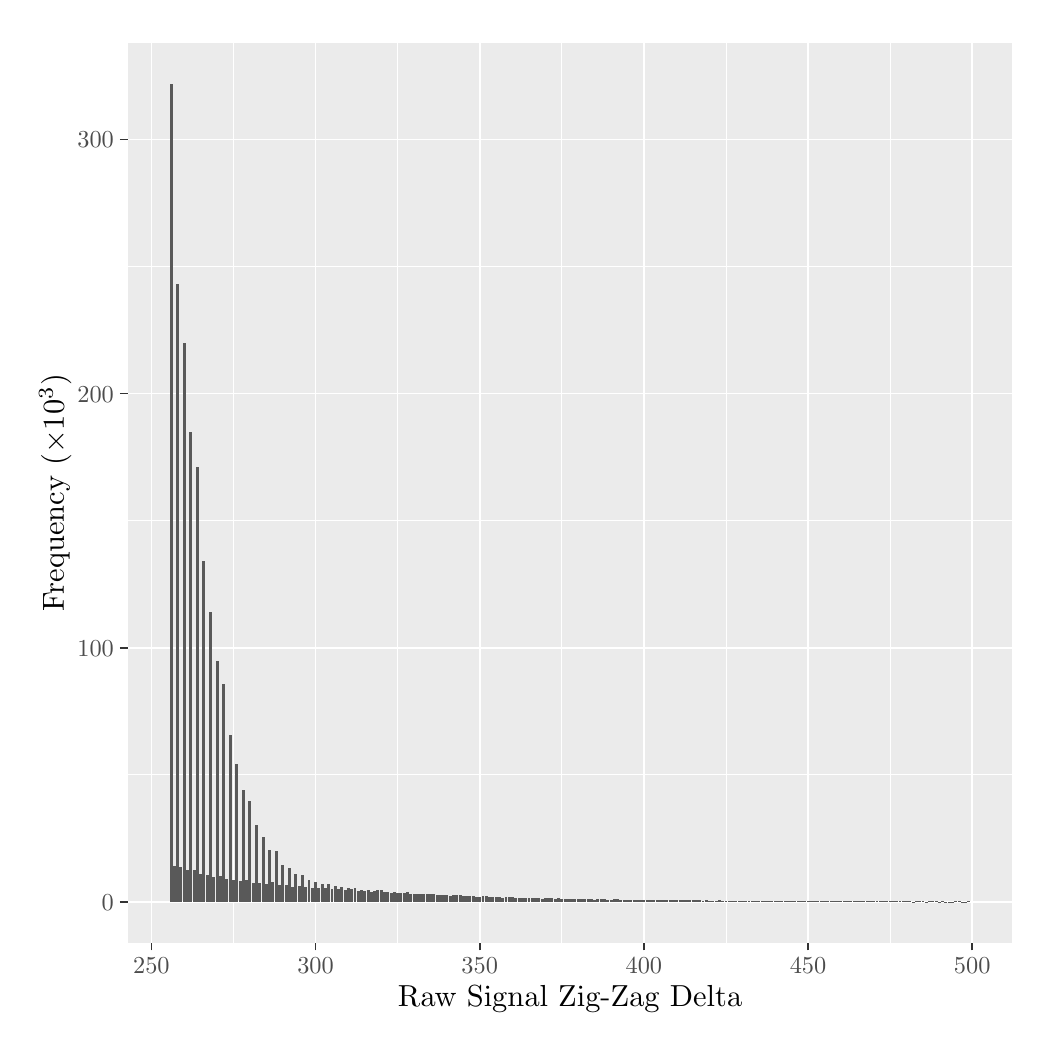
\begin{tikzpicture}[x=1pt,y=1pt]
\definecolor{fillColor}{RGB}{255,255,255}
\path[use as bounding box,fill=fillColor,fill opacity=0.00] (0,0) rectangle (361.35,361.35);
\begin{scope}
\path[clip] (  0.00,  0.00) rectangle (361.35,361.35);
\definecolor{drawColor}{RGB}{255,255,255}
\definecolor{fillColor}{RGB}{255,255,255}

\path[draw=drawColor,line width= 0.6pt,line join=round,line cap=round,fill=fillColor] (  0.00,  0.00) rectangle (361.35,361.35);
\end{scope}
\begin{scope}
\path[clip] ( 36.11, 30.69) rectangle (355.85,355.85);
\definecolor{fillColor}{gray}{0.92}

\path[fill=fillColor] ( 36.11, 30.69) rectangle (355.85,355.85);
\definecolor{drawColor}{RGB}{255,255,255}

\path[draw=drawColor,line width= 0.3pt,line join=round] ( 36.11, 91.37) --
	(355.85, 91.37);

\path[draw=drawColor,line width= 0.3pt,line join=round] ( 36.11,183.19) --
	(355.85,183.19);

\path[draw=drawColor,line width= 0.3pt,line join=round] ( 36.11,275.01) --
	(355.85,275.01);

\path[draw=drawColor,line width= 0.3pt,line join=round] ( 74.37, 30.69) --
	( 74.37,355.85);

\path[draw=drawColor,line width= 0.3pt,line join=round] (133.69, 30.69) --
	(133.69,355.85);

\path[draw=drawColor,line width= 0.3pt,line join=round] (193.01, 30.69) --
	(193.01,355.85);

\path[draw=drawColor,line width= 0.3pt,line join=round] (252.34, 30.69) --
	(252.34,355.85);

\path[draw=drawColor,line width= 0.3pt,line join=round] (311.66, 30.69) --
	(311.66,355.85);

\path[draw=drawColor,line width= 0.6pt,line join=round] ( 36.11, 45.47) --
	(355.85, 45.47);

\path[draw=drawColor,line width= 0.6pt,line join=round] ( 36.11,137.28) --
	(355.85,137.28);

\path[draw=drawColor,line width= 0.6pt,line join=round] ( 36.11,229.10) --
	(355.85,229.10);

\path[draw=drawColor,line width= 0.6pt,line join=round] ( 36.11,320.91) --
	(355.85,320.91);

\path[draw=drawColor,line width= 0.6pt,line join=round] ( 44.71, 30.69) --
	( 44.71,355.85);

\path[draw=drawColor,line width= 0.6pt,line join=round] (104.03, 30.69) --
	(104.03,355.85);

\path[draw=drawColor,line width= 0.6pt,line join=round] (163.35, 30.69) --
	(163.35,355.85);

\path[draw=drawColor,line width= 0.6pt,line join=round] (222.67, 30.69) --
	(222.67,355.85);

\path[draw=drawColor,line width= 0.6pt,line join=round] (282.00, 30.69) --
	(282.00,355.85);

\path[draw=drawColor,line width= 0.6pt,line join=round] (341.32, 30.69) --
	(341.32,355.85);
\definecolor{fillColor}{gray}{0.35}

\path[fill=fillColor] ( 51.30, 45.47) rectangle ( 52.37,341.07);

\path[fill=fillColor] ( 52.48, 45.47) rectangle ( 53.55, 58.32);

\path[fill=fillColor] ( 53.67, 45.47) rectangle ( 54.74,268.74);

\path[fill=fillColor] ( 54.86, 45.47) rectangle ( 55.92, 58.08);

\path[fill=fillColor] ( 56.04, 45.47) rectangle ( 57.11,247.36);

\path[fill=fillColor] ( 57.23, 45.47) rectangle ( 58.30, 56.94);

\path[fill=fillColor] ( 58.42, 45.47) rectangle ( 59.48,215.13);

\path[fill=fillColor] ( 59.60, 45.47) rectangle ( 60.67, 57.07);

\path[fill=fillColor] ( 60.79, 45.47) rectangle ( 61.86,202.50);

\path[fill=fillColor] ( 61.98, 45.47) rectangle ( 63.04, 55.42);

\path[fill=fillColor] ( 63.16, 45.47) rectangle ( 64.23,168.69);

\path[fill=fillColor] ( 64.35, 45.47) rectangle ( 65.42, 55.18);

\path[fill=fillColor] ( 65.53, 45.47) rectangle ( 66.60,150.14);

\path[fill=fillColor] ( 66.72, 45.47) rectangle ( 67.79, 54.37);

\path[fill=fillColor] ( 67.91, 45.47) rectangle ( 68.97,132.62);

\path[fill=fillColor] ( 69.09, 45.47) rectangle ( 70.16, 54.86);

\path[fill=fillColor] ( 70.28, 45.47) rectangle ( 71.35,124.30);

\path[fill=fillColor] ( 71.47, 45.47) rectangle ( 72.53, 53.65);

\path[fill=fillColor] ( 72.65, 45.47) rectangle ( 73.72,105.80);

\path[fill=fillColor] ( 73.84, 45.47) rectangle ( 74.91, 53.53);

\path[fill=fillColor] ( 75.03, 45.47) rectangle ( 76.09, 95.30);

\path[fill=fillColor] ( 76.21, 45.47) rectangle ( 77.28, 53.03);

\path[fill=fillColor] ( 77.40, 45.47) rectangle ( 78.47, 85.80);

\path[fill=fillColor] ( 78.58, 45.47) rectangle ( 79.65, 53.38);

\path[fill=fillColor] ( 79.77, 45.47) rectangle ( 80.84, 81.94);

\path[fill=fillColor] ( 80.96, 45.47) rectangle ( 82.03, 52.23);

\path[fill=fillColor] ( 82.14, 45.47) rectangle ( 83.21, 73.06);

\path[fill=fillColor] ( 83.33, 45.47) rectangle ( 84.40, 52.19);

\path[fill=fillColor] ( 84.52, 45.47) rectangle ( 85.58, 68.84);

\path[fill=fillColor] ( 85.70, 45.47) rectangle ( 86.77, 51.88);

\path[fill=fillColor] ( 86.89, 45.47) rectangle ( 87.96, 64.21);

\path[fill=fillColor] ( 88.08, 45.47) rectangle ( 89.14, 52.55);

\path[fill=fillColor] ( 89.26, 45.47) rectangle ( 90.33, 63.73);

\path[fill=fillColor] ( 90.45, 45.47) rectangle ( 91.52, 51.52);

\path[fill=fillColor] ( 91.64, 45.47) rectangle ( 92.70, 58.82);

\path[fill=fillColor] ( 92.82, 45.47) rectangle ( 93.89, 51.40);

\path[fill=fillColor] ( 94.01, 45.47) rectangle ( 95.08, 57.60);

\path[fill=fillColor] ( 95.19, 45.47) rectangle ( 96.26, 51.00);

\path[fill=fillColor] ( 96.38, 45.47) rectangle ( 97.45, 55.59);

\path[fill=fillColor] ( 97.57, 45.47) rectangle ( 98.64, 51.22);

\path[fill=fillColor] ( 98.75, 45.47) rectangle ( 99.82, 55.06);

\path[fill=fillColor] ( 99.94, 45.47) rectangle (101.01, 50.82);

\path[fill=fillColor] (101.13, 45.47) rectangle (102.19, 53.45);

\path[fill=fillColor] (102.31, 45.47) rectangle (103.38, 50.61);

\path[fill=fillColor] (103.50, 45.47) rectangle (104.57, 52.63);

\path[fill=fillColor] (104.69, 45.47) rectangle (105.75, 50.39);

\path[fill=fillColor] (105.87, 45.47) rectangle (106.94, 52.08);

\path[fill=fillColor] (107.06, 45.47) rectangle (108.13, 50.65);

\path[fill=fillColor] (108.25, 45.47) rectangle (109.31, 52.00);

\path[fill=fillColor] (109.43, 45.47) rectangle (110.50, 50.26);

\path[fill=fillColor] (110.62, 45.47) rectangle (111.69, 51.13);

\path[fill=fillColor] (111.80, 45.47) rectangle (112.87, 50.05);

\path[fill=fillColor] (112.99, 45.47) rectangle (114.06, 50.72);

\path[fill=fillColor] (114.18, 45.47) rectangle (115.25, 49.84);

\path[fill=fillColor] (115.36, 45.47) rectangle (116.43, 50.38);

\path[fill=fillColor] (116.55, 45.47) rectangle (117.62, 50.03);

\path[fill=fillColor] (117.74, 45.47) rectangle (118.80, 50.45);

\path[fill=fillColor] (118.92, 45.47) rectangle (119.99, 49.53);

\path[fill=fillColor] (120.11, 45.47) rectangle (121.18, 49.83);

\path[fill=fillColor] (121.30, 45.47) rectangle (122.36, 49.34);

\path[fill=fillColor] (122.48, 45.47) rectangle (123.55, 49.74);

\path[fill=fillColor] (123.67, 45.47) rectangle (124.74, 49.20);

\path[fill=fillColor] (124.86, 45.47) rectangle (125.92, 49.39);

\path[fill=fillColor] (126.04, 45.47) rectangle (127.11, 49.63);

\path[fill=fillColor] (127.23, 45.47) rectangle (128.30, 49.72);

\path[fill=fillColor] (128.41, 45.47) rectangle (129.48, 48.89);

\path[fill=fillColor] (129.60, 45.47) rectangle (130.67, 49.02);

\path[fill=fillColor] (130.79, 45.47) rectangle (131.85, 48.70);

\path[fill=fillColor] (131.97, 45.47) rectangle (133.04, 49.02);

\path[fill=fillColor] (133.16, 45.47) rectangle (134.23, 48.56);

\path[fill=fillColor] (134.35, 45.47) rectangle (135.41, 48.63);

\path[fill=fillColor] (135.53, 45.47) rectangle (136.60, 48.78);

\path[fill=fillColor] (136.72, 45.47) rectangle (137.79, 48.94);

\path[fill=fillColor] (137.91, 45.47) rectangle (138.97, 48.45);

\path[fill=fillColor] (139.09, 45.47) rectangle (140.16, 48.45);

\path[fill=fillColor] (140.28, 45.47) rectangle (141.35, 48.29);

\path[fill=fillColor] (141.46, 45.47) rectangle (142.53, 48.26);

\path[fill=fillColor] (142.65, 45.47) rectangle (143.72, 48.14);

\path[fill=fillColor] (143.84, 45.47) rectangle (144.91, 48.13);

\path[fill=fillColor] (145.02, 45.47) rectangle (146.09, 48.21);

\path[fill=fillColor] (146.21, 45.47) rectangle (147.28, 48.16);

\path[fill=fillColor] (147.40, 45.47) rectangle (148.46, 47.87);

\path[fill=fillColor] (148.58, 45.47) rectangle (149.65, 48.02);

\path[fill=fillColor] (149.77, 45.47) rectangle (150.84, 47.77);

\path[fill=fillColor] (150.96, 45.47) rectangle (152.02, 47.92);

\path[fill=fillColor] (152.14, 45.47) rectangle (153.21, 47.64);

\path[fill=fillColor] (153.33, 45.47) rectangle (154.40, 47.79);

\path[fill=fillColor] (154.52, 45.47) rectangle (155.58, 47.79);

\path[fill=fillColor] (155.70, 45.47) rectangle (156.77, 47.87);

\path[fill=fillColor] (156.89, 45.47) rectangle (157.96, 47.41);

\path[fill=fillColor] (158.07, 45.47) rectangle (159.14, 47.60);

\path[fill=fillColor] (159.26, 45.47) rectangle (160.33, 47.45);

\path[fill=fillColor] (160.45, 45.47) rectangle (161.52, 47.53);

\path[fill=fillColor] (161.63, 45.47) rectangle (162.70, 47.28);

\path[fill=fillColor] (162.82, 45.47) rectangle (163.89, 47.36);

\path[fill=fillColor] (164.01, 45.47) rectangle (165.07, 47.44);

\path[fill=fillColor] (165.19, 45.47) rectangle (166.26, 47.53);

\path[fill=fillColor] (166.38, 45.47) rectangle (167.45, 47.16);

\path[fill=fillColor] (167.57, 45.47) rectangle (168.63, 47.28);

\path[fill=fillColor] (168.75, 45.47) rectangle (169.82, 47.08);

\path[fill=fillColor] (169.94, 45.47) rectangle (171.01, 47.23);

\path[fill=fillColor] (171.13, 45.47) rectangle (172.19, 47.01);

\path[fill=fillColor] (172.31, 45.47) rectangle (173.38, 47.12);

\path[fill=fillColor] (173.50, 45.47) rectangle (174.57, 47.07);

\path[fill=fillColor] (174.68, 45.47) rectangle (175.75, 47.10);

\path[fill=fillColor] (175.87, 45.47) rectangle (176.94, 46.90);

\path[fill=fillColor] (177.06, 45.47) rectangle (178.13, 46.95);

\path[fill=fillColor] (178.24, 45.47) rectangle (179.31, 46.84);

\path[fill=fillColor] (179.43, 45.47) rectangle (180.50, 46.93);

\path[fill=fillColor] (180.62, 45.47) rectangle (181.68, 46.77);

\path[fill=fillColor] (181.80, 45.47) rectangle (182.87, 46.83);

\path[fill=fillColor] (182.99, 45.47) rectangle (184.06, 46.79);

\path[fill=fillColor] (184.18, 45.47) rectangle (185.24, 46.87);

\path[fill=fillColor] (185.36, 45.47) rectangle (186.43, 46.66);

\path[fill=fillColor] (186.55, 45.47) rectangle (187.62, 46.70);

\path[fill=fillColor] (187.74, 45.47) rectangle (188.80, 46.69);

\path[fill=fillColor] (188.92, 45.47) rectangle (189.99, 46.71);

\path[fill=fillColor] (190.11, 45.47) rectangle (191.18, 46.63);

\path[fill=fillColor] (191.29, 45.47) rectangle (192.36, 46.68);

\path[fill=fillColor] (192.48, 45.47) rectangle (193.55, 46.65);

\path[fill=fillColor] (193.67, 45.47) rectangle (194.73, 46.63);

\path[fill=fillColor] (194.85, 45.47) rectangle (195.92, 46.46);

\path[fill=fillColor] (196.04, 45.47) rectangle (197.11, 46.51);

\path[fill=fillColor] (197.23, 45.47) rectangle (198.29, 46.47);

\path[fill=fillColor] (198.41, 45.47) rectangle (199.48, 46.48);

\path[fill=fillColor] (199.60, 45.47) rectangle (200.67, 46.41);

\path[fill=fillColor] (200.79, 45.47) rectangle (201.85, 46.41);

\path[fill=fillColor] (201.97, 45.47) rectangle (203.04, 46.48);

\path[fill=fillColor] (203.16, 45.47) rectangle (204.23, 46.55);

\path[fill=fillColor] (204.34, 45.47) rectangle (205.41, 46.29);

\path[fill=fillColor] (205.53, 45.47) rectangle (206.60, 46.39);

\path[fill=fillColor] (206.72, 45.47) rectangle (207.79, 46.33);

\path[fill=fillColor] (207.90, 45.47) rectangle (208.97, 46.36);

\path[fill=fillColor] (209.09, 45.47) rectangle (210.16, 46.31);

\path[fill=fillColor] (210.28, 45.47) rectangle (211.34, 46.30);

\path[fill=fillColor] (211.46, 45.47) rectangle (212.53, 46.36);

\path[fill=fillColor] (212.65, 45.47) rectangle (213.72, 46.35);

\path[fill=fillColor] (213.84, 45.47) rectangle (214.90, 46.19);

\path[fill=fillColor] (215.02, 45.47) rectangle (216.09, 46.23);

\path[fill=fillColor] (216.21, 45.47) rectangle (217.28, 46.21);

\path[fill=fillColor] (217.40, 45.47) rectangle (218.46, 46.19);

\path[fill=fillColor] (218.58, 45.47) rectangle (219.65, 46.21);

\path[fill=fillColor] (219.77, 45.47) rectangle (220.84, 46.18);

\path[fill=fillColor] (220.95, 45.47) rectangle (222.02, 46.17);

\path[fill=fillColor] (222.14, 45.47) rectangle (223.21, 46.19);

\path[fill=fillColor] (223.33, 45.47) rectangle (224.40, 46.18);

\path[fill=fillColor] (224.51, 45.47) rectangle (225.58, 46.12);

\path[fill=fillColor] (225.70, 45.47) rectangle (226.77, 46.08);

\path[fill=fillColor] (226.89, 45.47) rectangle (227.95, 46.10);

\path[fill=fillColor] (228.07, 45.47) rectangle (229.14, 46.09);

\path[fill=fillColor] (229.26, 45.47) rectangle (230.33, 46.07);

\path[fill=fillColor] (230.45, 45.47) rectangle (231.51, 46.13);

\path[fill=fillColor] (231.63, 45.47) rectangle (232.70, 46.04);

\path[fill=fillColor] (232.82, 45.47) rectangle (233.89, 46.04);

\path[fill=fillColor] (234.01, 45.47) rectangle (235.07, 45.98);

\path[fill=fillColor] (235.19, 45.47) rectangle (236.26, 46.03);

\path[fill=fillColor] (236.38, 45.47) rectangle (237.45, 45.97);

\path[fill=fillColor] (237.56, 45.47) rectangle (238.63, 46.03);

\path[fill=fillColor] (238.75, 45.47) rectangle (239.82, 45.99);

\path[fill=fillColor] (239.94, 45.47) rectangle (241.01, 46.09);

\path[fill=fillColor] (241.12, 45.47) rectangle (242.19, 46.03);

\path[fill=fillColor] (242.31, 45.47) rectangle (243.38, 45.97);

\path[fill=fillColor] (243.50, 45.47) rectangle (244.56, 45.91);

\path[fill=fillColor] (244.68, 45.47) rectangle (245.75, 46.00);

\path[fill=fillColor] (245.87, 45.47) rectangle (246.94, 45.90);

\path[fill=fillColor] (247.06, 45.47) rectangle (248.12, 45.93);

\path[fill=fillColor] (248.24, 45.47) rectangle (249.31, 45.86);

\path[fill=fillColor] (249.43, 45.47) rectangle (250.50, 45.96);

\path[fill=fillColor] (250.61, 45.47) rectangle (251.68, 45.90);

\path[fill=fillColor] (251.80, 45.47) rectangle (252.87, 45.95);

\path[fill=fillColor] (252.99, 45.47) rectangle (254.06, 45.87);

\path[fill=fillColor] (254.17, 45.47) rectangle (255.24, 45.86);

\path[fill=fillColor] (255.36, 45.47) rectangle (256.43, 45.84);

\path[fill=fillColor] (256.55, 45.47) rectangle (257.61, 45.86);

\path[fill=fillColor] (257.73, 45.47) rectangle (258.80, 45.85);

\path[fill=fillColor] (258.92, 45.47) rectangle (259.99, 45.89);

\path[fill=fillColor] (260.11, 45.47) rectangle (261.17, 45.83);

\path[fill=fillColor] (261.29, 45.47) rectangle (262.36, 45.86);

\path[fill=fillColor] (262.48, 45.47) rectangle (263.55, 45.80);

\path[fill=fillColor] (263.67, 45.47) rectangle (264.73, 45.84);

\path[fill=fillColor] (264.85, 45.47) rectangle (265.92, 45.78);

\path[fill=fillColor] (266.04, 45.47) rectangle (267.11, 45.84);

\path[fill=fillColor] (267.22, 45.47) rectangle (268.29, 45.77);

\path[fill=fillColor] (268.41, 45.47) rectangle (269.48, 45.82);

\path[fill=fillColor] (269.60, 45.47) rectangle (270.67, 45.79);

\path[fill=fillColor] (270.78, 45.47) rectangle (271.85, 45.77);

\path[fill=fillColor] (271.97, 45.47) rectangle (273.04, 45.76);

\path[fill=fillColor] (273.16, 45.47) rectangle (274.22, 45.76);

\path[fill=fillColor] (274.34, 45.47) rectangle (275.41, 45.75);

\path[fill=fillColor] (275.53, 45.47) rectangle (276.60, 45.75);

\path[fill=fillColor] (276.72, 45.47) rectangle (277.78, 45.70);

\path[fill=fillColor] (277.90, 45.47) rectangle (278.97, 45.74);

\path[fill=fillColor] (279.09, 45.47) rectangle (280.16, 45.76);

\path[fill=fillColor] (280.28, 45.47) rectangle (281.34, 45.71);

\path[fill=fillColor] (281.46, 45.47) rectangle (282.53, 45.70);

\path[fill=fillColor] (282.65, 45.47) rectangle (283.72, 45.71);

\path[fill=fillColor] (283.83, 45.47) rectangle (284.90, 45.74);

\path[fill=fillColor] (285.02, 45.47) rectangle (286.09, 45.70);

\path[fill=fillColor] (286.21, 45.47) rectangle (287.28, 45.70);

\path[fill=fillColor] (287.39, 45.47) rectangle (288.46, 45.72);

\path[fill=fillColor] (288.58, 45.47) rectangle (289.65, 45.68);

\path[fill=fillColor] (289.77, 45.47) rectangle (290.83, 45.70);

\path[fill=fillColor] (290.95, 45.47) rectangle (292.02, 45.69);

\path[fill=fillColor] (292.14, 45.47) rectangle (293.21, 45.67);

\path[fill=fillColor] (293.33, 45.47) rectangle (294.39, 45.67);

\path[fill=fillColor] (294.51, 45.47) rectangle (295.58, 45.68);

\path[fill=fillColor] (295.70, 45.47) rectangle (296.77, 45.64);

\path[fill=fillColor] (296.89, 45.47) rectangle (297.95, 45.70);

\path[fill=fillColor] (298.07, 45.47) rectangle (299.14, 45.68);

\path[fill=fillColor] (299.26, 45.47) rectangle (300.33, 45.66);

\path[fill=fillColor] (300.44, 45.47) rectangle (301.51, 45.66);

\path[fill=fillColor] (301.63, 45.47) rectangle (302.70, 45.67);

\path[fill=fillColor] (302.82, 45.47) rectangle (303.89, 45.65);

\path[fill=fillColor] (304.00, 45.47) rectangle (305.07, 45.62);

\path[fill=fillColor] (305.19, 45.47) rectangle (306.26, 45.63);

\path[fill=fillColor] (306.38, 45.47) rectangle (307.44, 45.67);

\path[fill=fillColor] (307.56, 45.47) rectangle (308.63, 45.64);

\path[fill=fillColor] (308.75, 45.47) rectangle (309.82, 45.63);

\path[fill=fillColor] (309.94, 45.47) rectangle (311.00, 45.63);

\path[fill=fillColor] (311.12, 45.47) rectangle (312.19, 45.65);

\path[fill=fillColor] (312.31, 45.47) rectangle (313.38, 45.63);

\path[fill=fillColor] (313.49, 45.47) rectangle (314.56, 45.61);

\path[fill=fillColor] (314.68, 45.47) rectangle (315.75, 45.60);

\path[fill=fillColor] (315.87, 45.47) rectangle (316.94, 45.65);

\path[fill=fillColor] (317.05, 45.47) rectangle (318.12, 45.61);

\path[fill=fillColor] (318.24, 45.47) rectangle (319.31, 45.64);

\path[fill=fillColor] (319.43, 45.47) rectangle (320.49, 45.59);

\path[fill=fillColor] (320.61, 45.47) rectangle (321.68, 45.62);

\path[fill=fillColor] (321.80, 45.47) rectangle (322.87, 45.60);

\path[fill=fillColor] (322.99, 45.47) rectangle (324.05, 45.63);

\path[fill=fillColor] (324.17, 45.47) rectangle (325.24, 45.59);

\path[fill=fillColor] (325.36, 45.47) rectangle (326.43, 45.63);

\path[fill=fillColor] (326.55, 45.47) rectangle (327.61, 45.61);

\path[fill=fillColor] (327.73, 45.47) rectangle (328.80, 45.60);

\path[fill=fillColor] (328.92, 45.47) rectangle (329.99, 45.59);

\path[fill=fillColor] (330.10, 45.47) rectangle (331.17, 45.61);

\path[fill=fillColor] (331.29, 45.47) rectangle (332.36, 45.58);

\path[fill=fillColor] (332.48, 45.47) rectangle (333.55, 45.59);

\path[fill=fillColor] (333.66, 45.47) rectangle (334.73, 45.57);

\path[fill=fillColor] (334.85, 45.47) rectangle (335.92, 45.61);

\path[fill=fillColor] (336.04, 45.47) rectangle (337.10, 45.60);

\path[fill=fillColor] (337.22, 45.47) rectangle (338.29, 45.57);

\path[fill=fillColor] (338.41, 45.47) rectangle (339.48, 45.57);

\path[fill=fillColor] (339.60, 45.47) rectangle (340.66, 45.60);
\end{scope}
\begin{scope}
\path[clip] (  0.00,  0.00) rectangle (361.35,361.35);
\definecolor{drawColor}{gray}{0.30}

\node[text=drawColor,anchor=base east,inner sep=0pt, outer sep=0pt, scale=  0.88] at ( 31.16, 42.44) {0};

\node[text=drawColor,anchor=base east,inner sep=0pt, outer sep=0pt, scale=  0.88] at ( 31.16,134.25) {100};

\node[text=drawColor,anchor=base east,inner sep=0pt, outer sep=0pt, scale=  0.88] at ( 31.16,226.07) {200};

\node[text=drawColor,anchor=base east,inner sep=0pt, outer sep=0pt, scale=  0.88] at ( 31.16,317.88) {300};
\end{scope}
\begin{scope}
\path[clip] (  0.00,  0.00) rectangle (361.35,361.35);
\definecolor{drawColor}{gray}{0.20}

\path[draw=drawColor,line width= 0.6pt,line join=round] ( 33.36, 45.47) --
	( 36.11, 45.47);

\path[draw=drawColor,line width= 0.6pt,line join=round] ( 33.36,137.28) --
	( 36.11,137.28);

\path[draw=drawColor,line width= 0.6pt,line join=round] ( 33.36,229.10) --
	( 36.11,229.10);

\path[draw=drawColor,line width= 0.6pt,line join=round] ( 33.36,320.91) --
	( 36.11,320.91);
\end{scope}
\begin{scope}
\path[clip] (  0.00,  0.00) rectangle (361.35,361.35);
\definecolor{drawColor}{gray}{0.20}

\path[draw=drawColor,line width= 0.6pt,line join=round] ( 44.71, 27.94) --
	( 44.71, 30.69);

\path[draw=drawColor,line width= 0.6pt,line join=round] (104.03, 27.94) --
	(104.03, 30.69);

\path[draw=drawColor,line width= 0.6pt,line join=round] (163.35, 27.94) --
	(163.35, 30.69);

\path[draw=drawColor,line width= 0.6pt,line join=round] (222.67, 27.94) --
	(222.67, 30.69);

\path[draw=drawColor,line width= 0.6pt,line join=round] (282.00, 27.94) --
	(282.00, 30.69);

\path[draw=drawColor,line width= 0.6pt,line join=round] (341.32, 27.94) --
	(341.32, 30.69);
\end{scope}
\begin{scope}
\path[clip] (  0.00,  0.00) rectangle (361.35,361.35);
\definecolor{drawColor}{gray}{0.30}

\node[text=drawColor,anchor=base,inner sep=0pt, outer sep=0pt, scale=  0.88] at ( 44.71, 19.68) {250};

\node[text=drawColor,anchor=base,inner sep=0pt, outer sep=0pt, scale=  0.88] at (104.03, 19.68) {300};

\node[text=drawColor,anchor=base,inner sep=0pt, outer sep=0pt, scale=  0.88] at (163.35, 19.68) {350};

\node[text=drawColor,anchor=base,inner sep=0pt, outer sep=0pt, scale=  0.88] at (222.67, 19.68) {400};

\node[text=drawColor,anchor=base,inner sep=0pt, outer sep=0pt, scale=  0.88] at (282.00, 19.68) {450};

\node[text=drawColor,anchor=base,inner sep=0pt, outer sep=0pt, scale=  0.88] at (341.32, 19.68) {500};
\end{scope}
\begin{scope}
\path[clip] (  0.00,  0.00) rectangle (361.35,361.35);
\definecolor{drawColor}{RGB}{0,0,0}

\node[text=drawColor,anchor=base,inner sep=0pt, outer sep=0pt, scale=  1.10] at (195.98,  7.64) {Raw Signal Zig-Zag Delta};
\end{scope}
\begin{scope}
\path[clip] (  0.00,  0.00) rectangle (361.35,361.35);
\definecolor{drawColor}{RGB}{0,0,0}

\node[text=drawColor,rotate= 90.00,anchor=base,inner sep=0pt, outer sep=0pt, scale=  1.10] at ( 13.08,193.27) {Frequency ($\times 10^3$)};
\end{scope}
\end{tikzpicture}

	\caption{\label{fig:ex-hist}Histogram of the zig-zag delta exceptions up to 500. This figure is the tail of Figure \ref{fig:zd-hist}. The right and left tail of Figure \ref{fig:delta-hist} are `meshed' together during the zig-zag transformation causing the stripped pattern.}
\end{figure}


Another improvement we can make is on the storage of the exceptions' positions.
Since the positions are strictly increasing we can take the deltas between each
position and subtract one. This will result in smaller values which we can then
bit pack using 5 bits instead of 4 for the number of bits used.
5 instead of 4 bits are required to account for any outliers given the maximum
read length is roughly 6 million. If 4 bits were used only position deltas up to
$2^{2^{4}-1}-1=32767$ could be represented which is clearly short of 6 million.

The strategy which combines all of the above exception bit packing strategies
and still stores the regular one byte data we will name \textit{compact vbbe21}.
See Figure \ref{fig:vbbe21-compact} for a visual representation of this
encoding. Notice the byte boundary padding which aligns the one byte data to
byte boundaries for downstream compression methods. For implementation
simplicity consider a similar strategy which does not bit pack the number of
exceptions, bit packs the exception' positions and data using one byte for the
number of bits used rather than 5 and 4 respectively, and uses padding between
the exceptions' positions and data. We shall name this strategy the
\textit{regular vbbe21} encoding or \textit{vbbe21} for short. See Figure
\ref{fig:vbbe21} for a pictorial representation.

\begin{figure}
\centering\begin{tikzpicture}[node distance=0cm,start chain=1 going right] \footnotesize
  \tikzstyle{mytape}=[draw,minimum height=1.7cm]
	\node(A1)  [on chain=1,mytape,fill=blue!20] {$\underset{\text{of exceptions}}{\underbrace{\overbracket{b_e}^{\text{4 bits}}}_{\text{bits for number}}}$};
	\node(A2)  [on chain=1,mytape,fill=blue!20] {$\underset{\text{exceptions}}{\underbrace{\overbracket{\text{ }e\text{ }}^{b_e\text{ bits}}}_{\text{number of}}}$};
	\node(B1)  [on chain=1,mytape,fill=yellow!20] {$\underset{\text{position}}{\underbrace{\overbracket{b_p}^{5\text{ bits}}}_{\text{bits per exception}}}$};
	\node(B2)  [on chain=1,mytape,fill=yellow!20] {$\underbrace{\overbracket{p1,\delta(p_1,p_2,\dots,p_e)-1}^{b_pe\text{ bits}}}_{\text{exception positions}}$};
	\node(C1)  [on chain=1,mytape,fill=yellow!35] {$\underset{\text{byte exception}}{\underbrace{\overbracket{b_x}^{4\text{ bits}}}_{\text{bits per two}}}$};
	\node(C2)  [on chain=1,mytape,fill=yellow!35] {$\underbrace{\overbracket{(x_{p_1},x_{p_2},\dots,x_{p_e})-256}^{b_xe\text{ bits}}}_{\text{two byte exceptions}}$};
	\node [on chain=1,mytape,fill=gray!35] {$\underbrace{\overbracket{\text{ }\dots \text{ }}^{<1\text{ byte}}}_{\text{padding}}$};
	\node(D)  [on chain=1,mytape,fill=green!35] {$\underbrace{\overbracket{x_{q_1},x_{q_2},\dots,x_{q_{n-e}}}^{n-e\text{ bytes}}}_{\text{one byte data}}$};
\end{tikzpicture}
	\caption{\label{fig:vbbe21-compact}The compact vbbe21 encoding bit packs the
	number of exceptions, the deltas of the exceptions' positions and the
	two byte exceptions subtracted by 256. Less than one byte is used for
	padding to align the bit packed data to the next byte boundary. Then,
	the one byte data is recorded as in vbe21.}
\end{figure}

\section{One Byte, Two Byte Exceptions}
\label{sec:vbbe21}
%\begin{figure}
%\centering
	\begin{tikzpicture}[node distance=0cm,start chain=1 going right] \footnotesize
  \tikzstyle{mytape}=[draw,minimum height=1.5cm]
	\node(A1)  [on chain=1,mytape,fill=blue!20] {$\underset{\text{exceptions}}{\underbrace{\overbracket{\text{ }e\text{ }}^{\text{2 bytes}}}_{\text{number of}}}$};
	\node(A2)  [on chain=1,mytape,fill=yellow!20] {$\underbrace{\overbracket{p_1,p_2,\dots,p_e}^{4e\text{ bytes}}}_{\text{exception positions}}$};
	\node(A3)  [on chain=1,mytape,fill=yellow!35] {$\underbrace{\overbracket{x_{p_1},x_{p_2},\dots,x_{p_e}}^{2e\text{ bytes}}}_{\text{two byte exceptions}}$};
	\node(A4)  [on chain=1,mytape,fill=green!35] {$\underbrace{\overbracket{x_{q_1},x_{q_2},\dots,x_{q_{n-e}}}^{n-e\text{ bytes}}}_{\text{one byte data}}$};
\end{tikzpicture}
%	\caption[The vbe21 encoding.]{\label{fig:vbe21} The vbe21 encoding takes two byte integers
%	$x_1,x_2,\dots,x_n$ and encodes those which cannot fit into one byte as
%	\textit{exceptions} at the beginning of the stream. There are $e$
%	exceptions which are recorded by their original positions
%	$p_1,p_2,\dots,p_e$ and values $x_{p_1},x_{p_2},\dots,x_{p_e}$.
%	Following this is the regular one byte data where $q_i$ is the original
%	position of the $i$-th one byte data point. This is beneficial when
%	there are few exceptions in the data.}
%\end{figure}


The one byte, two byte exceptions encoding, abbreviated to \textit{vbe21},
encodes a list of integers using one byte for each integer except for integers
which cannot fit into one byte, known as \textit{exceptions}, which are encoded
using two bytes. See Figure \ref{fig:vbe21}. Rather than using a control code to
mark where normal data and exceptions occur as in the Stream VByte codec
(Section \ref{subsubsec:svb}), the exceptions are encoded at the beginning since
it is expected that exceptions will occur with small probability.

The number of exceptions is written using 2 bytes, followed by the exceptions'
positions in the list using 4 bytes each, the exceptions themselves using 2
bytes each and finally the regular one byte data. For example, consider the
sequence of integers $1024,12,10,4096,0,1,2,1024$. There are three
exceptions 1024, 4096 and 1024. Hence, vbe21 would use
\[ 2 + 3(4+2) + 8-3 = 25 \]
bytes for this sequence. See Figure \ref{fig:vbe21-eg}.

\begin{figure}
\centering\begin{tikzpicture}[node distance=0cm,start chain=1 going right,start chain=2 going right] \footnotesize
  \tikzstyle{mytape}=[draw,minimum height=1.4cm]
    \node(A1)  [on chain=1,mytape,fill=blue!20] {$\underbrace{\overbracket{\texttt{0x00}|\texttt{0x03}}^{\text{2 bytes}}}_{3}$};
    \node(A2)  [on chain=1,mytape,fill=yellow!20] {$\underbrace{\overbracket{\texttt{0x00}|\texttt{0x00}|\texttt{0x00}|\texttt{0x00}}^{\text{4 bytes}}}_{0}$};
    \node(A3)  [on chain=1,mytape,fill=yellow!20] {$\underbrace{\overbracket{\texttt{0x00}|\texttt{0x00}|\texttt{0x00}|\texttt{0x03}}^{\text{4 bytes}}}_{3}$};
    \node(A4)  [on chain=1,mytape,fill=yellow!20] {$\underbrace{\overbracket{\texttt{0x00}|\texttt{0x00}|\texttt{0x00}|\texttt{0x07}}^{\text{4 bytes}}}_{7}$};
    \node(B1)  [on chain=2,mytape,fill=yellow!35,below of=A1,node distance=1.4cm] {$\underbrace{\overbracket{\texttt{0x04}|\texttt{0x00}}^{\text{2 bytes}}}_{1024}$};
    \node(B2)  [on chain=2,mytape,fill=yellow!35] {$\underbrace{\overbracket{\texttt{0x10}|\texttt{0x00}}^{\text{2 bytes}}}_{\num{4096}}$};
    \node(B3)  [on chain=2,mytape,fill=yellow!35] {$\underbrace{\overbracket{\texttt{0x04}|\texttt{0x00}}^{\text{2 bytes}}}_{1024}$};
    \node(B4)  [on chain=2,mytape,fill=green!35] {$\underbrace{\overbracket{\texttt{0x0c}}^{\text{1 byte}}}_{12}$};
    \node(B5)  [on chain=2,mytape,fill=green!35] {$\underbrace{\overbracket{\texttt{0x0a}}^{\text{1 byte}}}_{10}$};
    \node(B6)  [on chain=2,mytape,fill=green!35] {$\underbrace{\overbracket{\texttt{0x00}}^{\text{1 byte}}}_{0}$};
    \node(B7)  [on chain=2,mytape,fill=green!35] {$\underbrace{\overbracket{\texttt{0x01}}^{\text{1 byte}}}_{1}$};
    \node(B8)  [on chain=2,mytape,fill=green!35] {$\underbrace{\overbracket{\texttt{0x02}}^{\text{1 byte}}}_{2}$};
\end{tikzpicture}

	\caption[An example of $1024,12,10,4096, 0,1,2,1024$ encoded with vbe21.]{\label{fig:vbe21-eg} An example of $1024,12,10,4096,
	0,1,2,1024$ encoded with vbe21. The encoding order is read from left to
	right and top to bottom. There are 3 exceptions located at positions 0,
	3 and 7 with values 1024, 4096 and 1024. It uses 25 bytes in total.}
\end{figure}


Now, consider applying encoding $A$ to a read. Let $C_A:\Omega\to\mathbb{N}_0$
be a random variable measuring the resulting compressed size in bytes where
$\Omega$ is the space of possible nanopore reads. Then
\begin{align*}
	C_{vbe21} &= \text{exceptions} + \text{one byte data}\\
	&= (2 + 6X) + (N - X)\\
	&= 2 + 5X + N
\end{align*}
where $N$ and $X$ are random variables measuring the read length and number of
exceptions respectively. Recall from Section \ref{subsec:prob} that the
probability that a zig-zag delta is greater than 255 and therefore outside the one
byte range is $\sim 5\times 10^{-5}$ for the data. Thus, the expected number of
zig-zag delta exceptions is
\[ E[X] = (5 \times 10^{-5})E[N] \]
%Also, the read lengths can be modelled by the Gamma distribution $\Gamma(1.0885,0.0096)$.
where the expected read length is
\[ E[N] = 113471.4 \]
from Table \ref{tab:n}. So $E[X] \approx 5.67$, that is we expect roughly 5 to 6
exceptions per read when using the zig-zag delta transformation.
Then, the expected compressed size is given by
\begin{align*}
	E[C_{vbe21-zd}] &= 2 + (2.5\times 10^{-4})E[N]+ E[N]\\
	&= 2 + 1.00025E[N]\\
	&\approx 113502 \text{ bytes}
\end{align*}
where vbe21-zd means first apply the zig-zag delta encoding then vbe21. In
comparison, using the Stream VByte 16 (or \textit{svb16}) encoding, the
compressed size is given by
\begin{align*}
	C_{svb16} &= \lceil N/8 \rceil + 2X + (N - X)\\
	&= \lceil N/8 \rceil + X + N.
\end{align*}
Then, the expected compressed size is
\begin{align*}
	E[C_{svb16-zd}] &= \lceil E[N]/8 \rceil + (5 \times 10^{-5})E[N] + E[N]\\
	&= \lceil E[N]/8 \rceil + 1.00005E[N]\\
	&\approx 127661 \text{ bytes}\\
	&> E[C_{vbe21-zd}].
\end{align*}

This translates into roughly 8 bits per data point for vbe21-zd versus
9 for svb16-zd.
%See Table \ref{tab:vbe21-bpp}.
Intuitively these numbers make sense considering vbe21-zd essentially represents
most points using one byte each and svb16-zd stores one extra bit per point in
the control byte section.  Compare this to the entropy of the data which is 7.70
bits per point or 5.39 for the zig-zag deltas. So it is clear that
vbe21-zd saves more space than svb16-zd: roughly 14 KiB on average per read or
an estimated 6.6 GiB for the whole data set. However, this is merely a container
for the data which is useful for downstream compression; alone it doesn't
provide great compression results as is obvious when comparing it to the entropy
of the data.

vbe21-zd is linear in time complexity during encoding since it requires
applying the zig-zag delta transformation and checking which values are
exceptions. The same is true for decoding and the svb16-zd codec.

%\begin{table}
    \caption{\label{tab:vbe21-bpp} The theoretical expected bits per point for the
vbe21-zd and svb16-zd encodings.}
    \begin{tabular}{|l|l|}
        \hline
Encoding & Expected Bits Per Point\\
        \hline
vbe21-zd & 8\\
svb16-zd & 9\\
	\hline
    \end{tabular}
\end{table}


\subsection{Exceptions Encoding}

There are better ways of storing the exceptions than in the raw sequential
format of vbe21.
As we have seen there are usually 5 to 6 exceptions per read meaning that
storing the number of exceptions using two bytes which has a range of 0 to 65535
for all reads is wasteful.
In particular, the number of exceptions per read ranges from 0 to 3616 but 99\%
of reads have between 0 and 42 exceptions. See Table \ref{tab:ex}. Its
distribution, shown in Figure \ref{fig:nex-hist}, could be nicely fitted by an
exponential distribution. In fact, around 20\% of the reads have no exceptions
at all.

\begin{table}
    \caption{\label{tab:ex} Summary statistics of the number of exceptions per read and the zig-zag delta exceptions themselves in the data.}
	\begin{tabular}{|l|m{1.8cm}|l|}
	    \hline
	    Statistic & Number of Exceptions Per Read & Exceptions\\
        \hline
		Min &0 & 256\\
		Q1 & 1& 260\\

		Q2 & 3& 266\\
		Q3 & 6& 278\\
		Max & 3616& 2317\\
\hline
		Mean & 4.8546&277.0465\\
		Mode & 0&256\\
		SD & 18.0595&36.8207\\
	\hline
    \end{tabular}
\end{table}

\begin{figure}
	\centering
% Created by tikzDevice version 0.12.3.1 on 2022-10-11 18:23:57
% !TEX encoding = UTF-8 Unicode
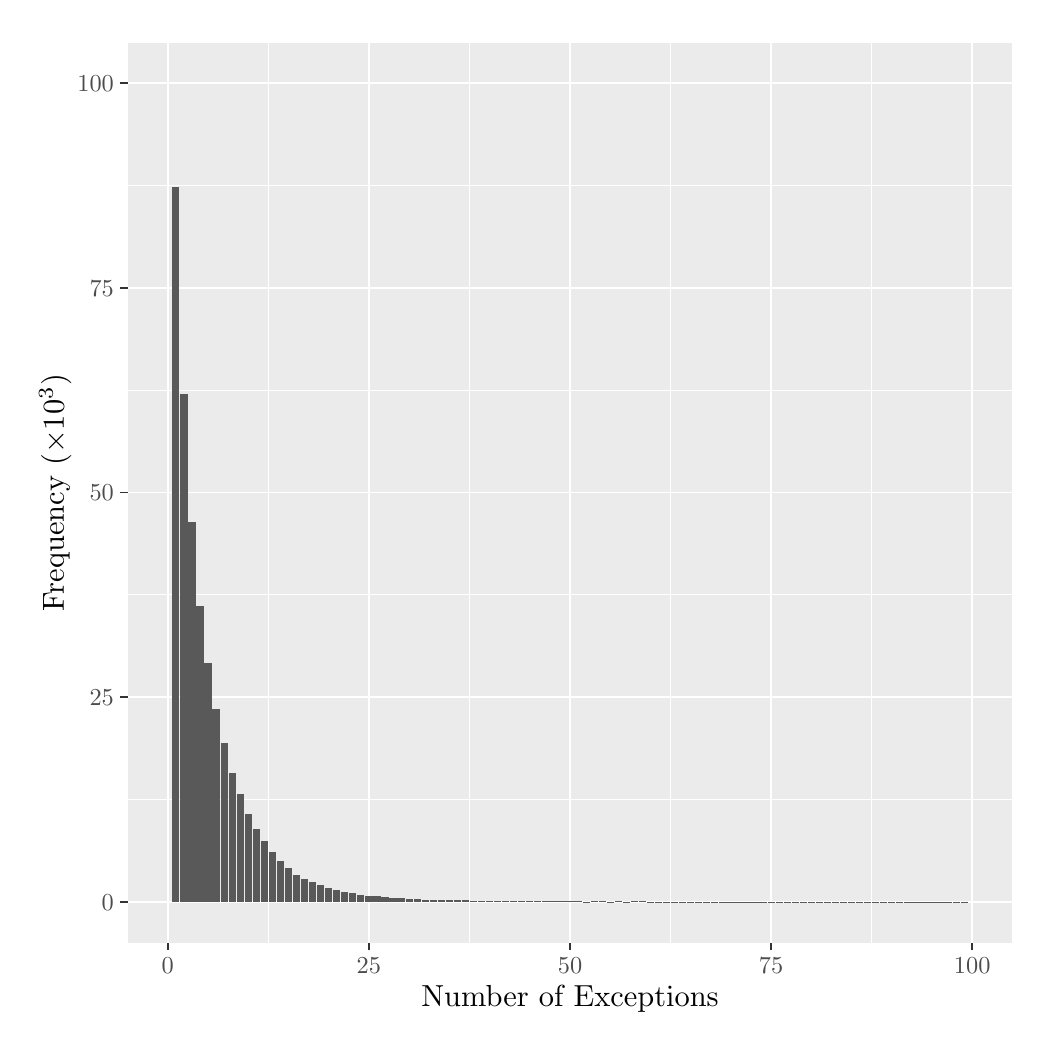
\begin{tikzpicture}[x=1pt,y=1pt]
\definecolor{fillColor}{RGB}{255,255,255}
\path[use as bounding box,fill=fillColor,fill opacity=0.00] (0,0) rectangle (361.35,361.35);
\begin{scope}
\path[clip] (  0.00,  0.00) rectangle (361.35,361.35);
\definecolor{drawColor}{RGB}{255,255,255}
\definecolor{fillColor}{RGB}{255,255,255}

\path[draw=drawColor,line width= 0.6pt,line join=round,line cap=round,fill=fillColor] (  0.00,  0.00) rectangle (361.35,361.35);
\end{scope}
\begin{scope}
\path[clip] ( 36.11, 30.69) rectangle (355.85,355.85);
\definecolor{fillColor}{gray}{0.92}

\path[fill=fillColor] ( 36.11, 30.69) rectangle (355.85,355.85);
\definecolor{drawColor}{RGB}{255,255,255}

\path[draw=drawColor,line width= 0.3pt,line join=round] ( 36.11, 82.45) --
	(355.85, 82.45);

\path[draw=drawColor,line width= 0.3pt,line join=round] ( 36.11,156.42) --
	(355.85,156.42);

\path[draw=drawColor,line width= 0.3pt,line join=round] ( 36.11,230.38) --
	(355.85,230.38);

\path[draw=drawColor,line width= 0.3pt,line join=round] ( 36.11,304.35) --
	(355.85,304.35);

\path[draw=drawColor,line width= 0.3pt,line join=round] ( 86.98, 30.69) --
	( 86.98,355.85);

\path[draw=drawColor,line width= 0.3pt,line join=round] (159.65, 30.69) --
	(159.65,355.85);

\path[draw=drawColor,line width= 0.3pt,line join=round] (232.31, 30.69) --
	(232.31,355.85);

\path[draw=drawColor,line width= 0.3pt,line join=round] (304.98, 30.69) --
	(304.98,355.85);

\path[draw=drawColor,line width= 0.6pt,line join=round] ( 36.11, 45.47) --
	(355.85, 45.47);

\path[draw=drawColor,line width= 0.6pt,line join=round] ( 36.11,119.43) --
	(355.85,119.43);

\path[draw=drawColor,line width= 0.6pt,line join=round] ( 36.11,193.40) --
	(355.85,193.40);

\path[draw=drawColor,line width= 0.6pt,line join=round] ( 36.11,267.37) --
	(355.85,267.37);

\path[draw=drawColor,line width= 0.6pt,line join=round] ( 36.11,341.34) --
	(355.85,341.34);

\path[draw=drawColor,line width= 0.6pt,line join=round] ( 50.64, 30.69) --
	( 50.64,355.85);

\path[draw=drawColor,line width= 0.6pt,line join=round] (123.31, 30.69) --
	(123.31,355.85);

\path[draw=drawColor,line width= 0.6pt,line join=round] (195.98, 30.69) --
	(195.98,355.85);

\path[draw=drawColor,line width= 0.6pt,line join=round] (268.65, 30.69) --
	(268.65,355.85);

\path[draw=drawColor,line width= 0.6pt,line join=round] (341.32, 30.69) --
	(341.32,355.85);
\definecolor{fillColor}{gray}{0.35}

\path[fill=fillColor] ( 52.24, 45.47) rectangle ( 54.86,303.76);

\path[fill=fillColor] ( 55.15, 45.47) rectangle ( 57.77,229.02);

\path[fill=fillColor] ( 58.06, 45.47) rectangle ( 60.67,182.55);

\path[fill=fillColor] ( 60.96, 45.47) rectangle ( 63.58,152.28);

\path[fill=fillColor] ( 63.87, 45.47) rectangle ( 66.49,131.71);

\path[fill=fillColor] ( 66.78, 45.47) rectangle ( 69.39,115.27);

\path[fill=fillColor] ( 69.68, 45.47) rectangle ( 72.30,103.03);

\path[fill=fillColor] ( 72.59, 45.47) rectangle ( 75.21, 92.15);

\path[fill=fillColor] ( 75.50, 45.47) rectangle ( 78.11, 84.47);

\path[fill=fillColor] ( 78.40, 45.47) rectangle ( 81.02, 77.36);

\path[fill=fillColor] ( 81.31, 45.47) rectangle ( 83.93, 71.87);

\path[fill=fillColor] ( 84.22, 45.47) rectangle ( 86.83, 67.43);

\path[fill=fillColor] ( 87.12, 45.47) rectangle ( 89.74, 63.64);

\path[fill=fillColor] ( 90.03, 45.47) rectangle ( 92.65, 60.19);

\path[fill=fillColor] ( 92.94, 45.47) rectangle ( 95.55, 57.70);

\path[fill=fillColor] ( 95.84, 45.47) rectangle ( 98.46, 55.08);

\path[fill=fillColor] ( 98.75, 45.47) rectangle (101.37, 53.84);

\path[fill=fillColor] (101.66, 45.47) rectangle (104.27, 52.65);

\path[fill=fillColor] (104.56, 45.47) rectangle (107.18, 51.51);

\path[fill=fillColor] (107.47, 45.47) rectangle (110.09, 50.42);

\path[fill=fillColor] (110.38, 45.47) rectangle (112.99, 49.62);

\path[fill=fillColor] (113.28, 45.47) rectangle (115.90, 48.95);

\path[fill=fillColor] (116.19, 45.47) rectangle (118.81, 48.54);

\path[fill=fillColor] (119.10, 45.47) rectangle (121.71, 48.05);

\path[fill=fillColor] (122.00, 45.47) rectangle (124.62, 47.58);

\path[fill=fillColor] (124.91, 45.47) rectangle (127.53, 47.40);

\path[fill=fillColor] (127.82, 45.47) rectangle (130.43, 47.26);

\path[fill=fillColor] (130.72, 45.47) rectangle (133.34, 46.87);

\path[fill=fillColor] (133.63, 45.47) rectangle (136.25, 46.79);

\path[fill=fillColor] (136.54, 45.47) rectangle (139.15, 46.48);

\path[fill=fillColor] (139.44, 45.47) rectangle (142.06, 46.53);

\path[fill=fillColor] (142.35, 45.47) rectangle (144.97, 46.31);

\path[fill=fillColor] (145.26, 45.47) rectangle (147.87, 46.29);

\path[fill=fillColor] (148.17, 45.47) rectangle (150.78, 46.20);

\path[fill=fillColor] (151.07, 45.47) rectangle (153.69, 46.11);

\path[fill=fillColor] (153.98, 45.47) rectangle (156.59, 45.98);

\path[fill=fillColor] (156.89, 45.47) rectangle (159.50, 46.01);

\path[fill=fillColor] (159.79, 45.47) rectangle (162.41, 45.94);

\path[fill=fillColor] (162.70, 45.47) rectangle (165.31, 45.80);

\path[fill=fillColor] (165.61, 45.47) rectangle (168.22, 45.91);

\path[fill=fillColor] (168.51, 45.47) rectangle (171.13, 45.81);

\path[fill=fillColor] (171.42, 45.47) rectangle (174.03, 45.73);

\path[fill=fillColor] (174.33, 45.47) rectangle (176.94, 45.84);

\path[fill=fillColor] (177.23, 45.47) rectangle (179.85, 45.73);

\path[fill=fillColor] (180.14, 45.47) rectangle (182.76, 45.74);

\path[fill=fillColor] (183.05, 45.47) rectangle (185.66, 45.74);

\path[fill=fillColor] (185.95, 45.47) rectangle (188.57, 45.67);

\path[fill=fillColor] (188.86, 45.47) rectangle (191.48, 45.69);

\path[fill=fillColor] (191.77, 45.47) rectangle (194.38, 45.65);

\path[fill=fillColor] (194.67, 45.47) rectangle (197.29, 45.68);

\path[fill=fillColor] (197.58, 45.47) rectangle (200.20, 45.71);

\path[fill=fillColor] (200.49, 45.47) rectangle (203.10, 45.59);

\path[fill=fillColor] (203.39, 45.47) rectangle (206.01, 45.66);

\path[fill=fillColor] (206.30, 45.47) rectangle (208.92, 45.63);

\path[fill=fillColor] (209.21, 45.47) rectangle (211.82, 45.59);

\path[fill=fillColor] (212.11, 45.47) rectangle (214.73, 45.60);

\path[fill=fillColor] (215.02, 45.47) rectangle (217.64, 45.58);

\path[fill=fillColor] (217.93, 45.47) rectangle (220.54, 45.62);

\path[fill=fillColor] (220.83, 45.47) rectangle (223.45, 45.60);

\path[fill=fillColor] (223.74, 45.47) rectangle (226.36, 45.55);

\path[fill=fillColor] (226.65, 45.47) rectangle (229.26, 45.57);

\path[fill=fillColor] (229.55, 45.47) rectangle (232.17, 45.55);

\path[fill=fillColor] (232.46, 45.47) rectangle (235.08, 45.56);

\path[fill=fillColor] (235.37, 45.47) rectangle (237.98, 45.56);

\path[fill=fillColor] (238.27, 45.47) rectangle (240.89, 45.55);

\path[fill=fillColor] (241.18, 45.47) rectangle (243.80, 45.52);

\path[fill=fillColor] (244.09, 45.47) rectangle (246.70, 45.53);

\path[fill=fillColor] (246.99, 45.47) rectangle (249.61, 45.57);

\path[fill=fillColor] (249.90, 45.47) rectangle (252.52, 45.54);

\path[fill=fillColor] (252.81, 45.47) rectangle (255.42, 45.54);

\path[fill=fillColor] (255.71, 45.47) rectangle (258.33, 45.53);

\path[fill=fillColor] (258.62, 45.47) rectangle (261.24, 45.51);

\path[fill=fillColor] (261.53, 45.47) rectangle (264.14, 45.53);

\path[fill=fillColor] (264.43, 45.47) rectangle (267.05, 45.50);

\path[fill=fillColor] (267.34, 45.47) rectangle (269.96, 45.52);

\path[fill=fillColor] (270.25, 45.47) rectangle (272.86, 45.53);

\path[fill=fillColor] (273.15, 45.47) rectangle (275.77, 45.53);

\path[fill=fillColor] (276.06, 45.47) rectangle (278.68, 45.51);

\path[fill=fillColor] (278.97, 45.47) rectangle (281.58, 45.53);

\path[fill=fillColor] (281.87, 45.47) rectangle (284.49, 45.53);

\path[fill=fillColor] (284.78, 45.47) rectangle (287.40, 45.50);

\path[fill=fillColor] (287.69, 45.47) rectangle (290.30, 45.50);

\path[fill=fillColor] (290.59, 45.47) rectangle (293.21, 45.49);

\path[fill=fillColor] (293.50, 45.47) rectangle (296.12, 45.51);

\path[fill=fillColor] (296.41, 45.47) rectangle (299.02, 45.50);

\path[fill=fillColor] (299.31, 45.47) rectangle (301.93, 45.53);

\path[fill=fillColor] (302.22, 45.47) rectangle (304.84, 45.51);

\path[fill=fillColor] (305.13, 45.47) rectangle (307.74, 45.51);

\path[fill=fillColor] (308.03, 45.47) rectangle (310.65, 45.51);

\path[fill=fillColor] (310.94, 45.47) rectangle (313.56, 45.50);

\path[fill=fillColor] (313.85, 45.47) rectangle (316.46, 45.50);

\path[fill=fillColor] (316.75, 45.47) rectangle (319.37, 45.53);

\path[fill=fillColor] (319.66, 45.47) rectangle (322.28, 45.50);

\path[fill=fillColor] (322.57, 45.47) rectangle (325.18, 45.50);

\path[fill=fillColor] (325.47, 45.47) rectangle (328.09, 45.51);

\path[fill=fillColor] (328.38, 45.47) rectangle (331.00, 45.50);

\path[fill=fillColor] (331.29, 45.47) rectangle (333.90, 45.51);

\path[fill=fillColor] (334.19, 45.47) rectangle (336.81, 45.50);

\path[fill=fillColor] (337.10, 45.47) rectangle (339.72, 45.49);
\end{scope}
\begin{scope}
\path[clip] (  0.00,  0.00) rectangle (361.35,361.35);
\definecolor{drawColor}{gray}{0.30}

\node[text=drawColor,anchor=base east,inner sep=0pt, outer sep=0pt, scale=  0.88] at ( 31.16, 42.44) {0};

\node[text=drawColor,anchor=base east,inner sep=0pt, outer sep=0pt, scale=  0.88] at ( 31.16,116.40) {25};

\node[text=drawColor,anchor=base east,inner sep=0pt, outer sep=0pt, scale=  0.88] at ( 31.16,190.37) {50};

\node[text=drawColor,anchor=base east,inner sep=0pt, outer sep=0pt, scale=  0.88] at ( 31.16,264.34) {75};

\node[text=drawColor,anchor=base east,inner sep=0pt, outer sep=0pt, scale=  0.88] at ( 31.16,338.31) {100};
\end{scope}
\begin{scope}
\path[clip] (  0.00,  0.00) rectangle (361.35,361.35);
\definecolor{drawColor}{gray}{0.20}

\path[draw=drawColor,line width= 0.6pt,line join=round] ( 33.36, 45.47) --
	( 36.11, 45.47);

\path[draw=drawColor,line width= 0.6pt,line join=round] ( 33.36,119.43) --
	( 36.11,119.43);

\path[draw=drawColor,line width= 0.6pt,line join=round] ( 33.36,193.40) --
	( 36.11,193.40);

\path[draw=drawColor,line width= 0.6pt,line join=round] ( 33.36,267.37) --
	( 36.11,267.37);

\path[draw=drawColor,line width= 0.6pt,line join=round] ( 33.36,341.34) --
	( 36.11,341.34);
\end{scope}
\begin{scope}
\path[clip] (  0.00,  0.00) rectangle (361.35,361.35);
\definecolor{drawColor}{gray}{0.20}

\path[draw=drawColor,line width= 0.6pt,line join=round] ( 50.64, 27.94) --
	( 50.64, 30.69);

\path[draw=drawColor,line width= 0.6pt,line join=round] (123.31, 27.94) --
	(123.31, 30.69);

\path[draw=drawColor,line width= 0.6pt,line join=round] (195.98, 27.94) --
	(195.98, 30.69);

\path[draw=drawColor,line width= 0.6pt,line join=round] (268.65, 27.94) --
	(268.65, 30.69);

\path[draw=drawColor,line width= 0.6pt,line join=round] (341.32, 27.94) --
	(341.32, 30.69);
\end{scope}
\begin{scope}
\path[clip] (  0.00,  0.00) rectangle (361.35,361.35);
\definecolor{drawColor}{gray}{0.30}

\node[text=drawColor,anchor=base,inner sep=0pt, outer sep=0pt, scale=  0.88] at ( 50.64, 19.68) {0};

\node[text=drawColor,anchor=base,inner sep=0pt, outer sep=0pt, scale=  0.88] at (123.31, 19.68) {25};

\node[text=drawColor,anchor=base,inner sep=0pt, outer sep=0pt, scale=  0.88] at (195.98, 19.68) {50};

\node[text=drawColor,anchor=base,inner sep=0pt, outer sep=0pt, scale=  0.88] at (268.65, 19.68) {75};

\node[text=drawColor,anchor=base,inner sep=0pt, outer sep=0pt, scale=  0.88] at (341.32, 19.68) {100};
\end{scope}
\begin{scope}
\path[clip] (  0.00,  0.00) rectangle (361.35,361.35);
\definecolor{drawColor}{RGB}{0,0,0}

\node[text=drawColor,anchor=base,inner sep=0pt, outer sep=0pt, scale=  1.10] at (195.98,  7.64) {Number of Exceptions};
\end{scope}
\begin{scope}
\path[clip] (  0.00,  0.00) rectangle (361.35,361.35);
\definecolor{drawColor}{RGB}{0,0,0}

\node[text=drawColor,rotate= 90.00,anchor=base,inner sep=0pt, outer sep=0pt, scale=  1.10] at ( 13.08,193.27) {Frequency ($\times 10^3$)};
\end{scope}
\end{tikzpicture}

	\caption{\label{fig:nex-hist}Histogram of the number of exceptions per read up to 100 which appears to nicely follow an exponential distribution. Values after 100 occur highly infrequently -- there are only 546 out of \num{500000} reads with more than 100 exceptions.}
\end{figure}


Instead of storing two bytes for the number of exceptions we can bit pack the
number of exceptions using four bits to represent the number of bits used.
Refer back to Section \ref{sec:bitpack} for a review of bit packing.
The maximum number of exceptions, 3616, requires at least
12 bits to represent it. Using the bit packing approach, $4+12=16$ bits or two
bytes would be used to represent it -- which is equivalent to the naive
approach. That is, in the worst case bit packing use the same space as the naive
approach. In the best case when there are zero exceptions only four bits are
required, and as long as there are lesser than 16 exceptions up to one byte is
used. Although this approach clearly saves space, we are talking about saving at
most 12 bits which is miniscule compared to the scale of the data.

Similarly, we can store the exceptions' data in a more compact form.
The exceptions themselves range from 256 to 2317 but 99\%
of the exceptions do not go higher than 481. The mean and mode are $\sim$277 and
256 respectively. Refer to Table \ref{tab:ex} for a summary and Figure
\ref{fig:ex-hist} for the histogram. Notably, the frequency of even-numbered
exceptions is much greater than adjacent odd-numbered exceptions from 256 up to
$\sim$330. This is due to large positive deltas occuring more frequently than
large negative deltas as previously discussed in Section \ref{subsec:stripe}.
One simple approach to encoding the exceptions is to subtract 256 since this is
the minimum exception value and then apply bit packing using 4 bits as before. The
average exception can then be represented using
0 to 5 bits which is better than the naive 16-bit per exception encoding. This
results in an expected improvement of $(16-5)\times 5-4=51$ bits per read.
In the worst case, the number of bits used per exception for this data will be 12
or $4 + 12e$ in total, which is better than the naive approach for $e>1$ and
equivalent for $e=1$. The implications of this is that bit packing the
exceptions' data never consumes more space than the naive strategy.

\begin{figure}
	\centering
% Created by tikzDevice version 0.12.3.1 on 2022-10-11 17:28:28
% !TEX encoding = UTF-8 Unicode
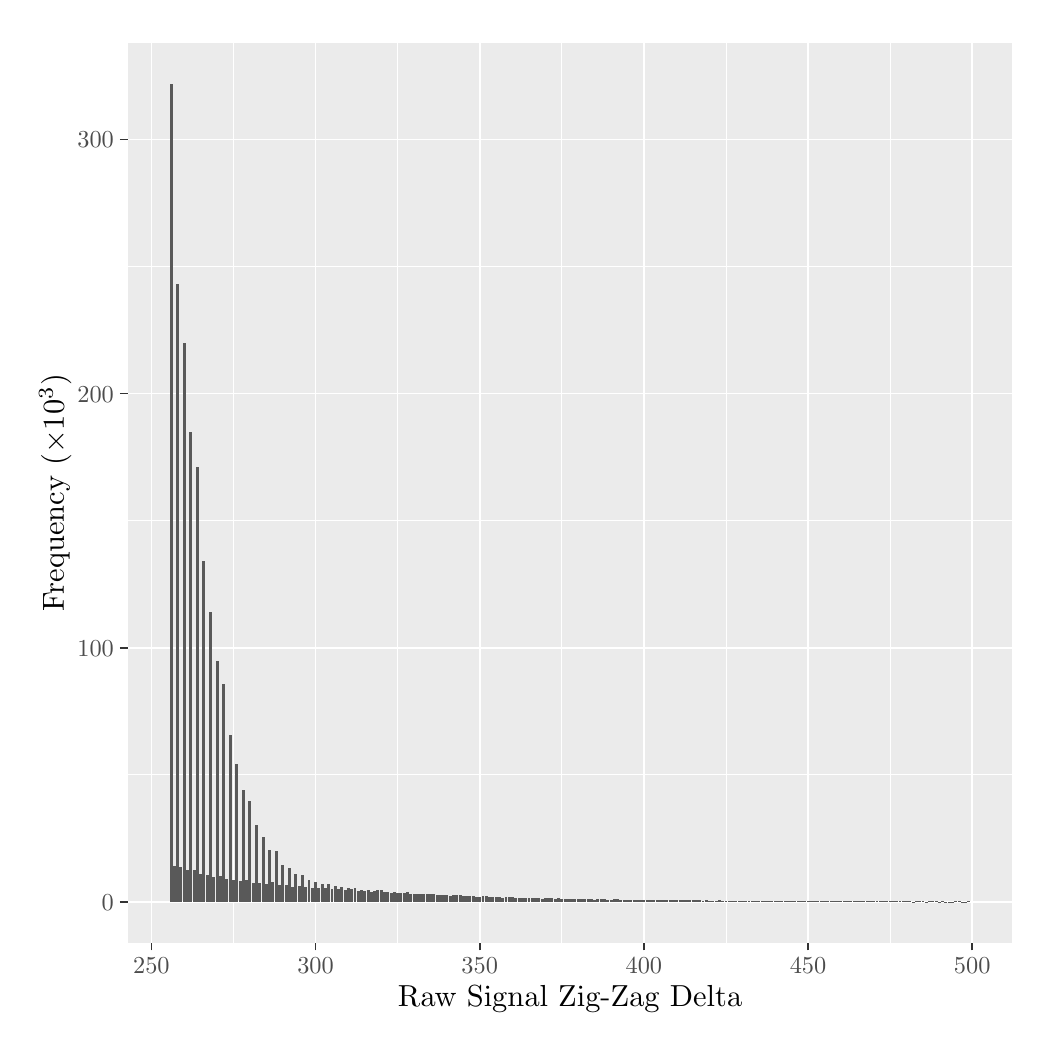
\begin{tikzpicture}[x=1pt,y=1pt]
\definecolor{fillColor}{RGB}{255,255,255}
\path[use as bounding box,fill=fillColor,fill opacity=0.00] (0,0) rectangle (361.35,361.35);
\begin{scope}
\path[clip] (  0.00,  0.00) rectangle (361.35,361.35);
\definecolor{drawColor}{RGB}{255,255,255}
\definecolor{fillColor}{RGB}{255,255,255}

\path[draw=drawColor,line width= 0.6pt,line join=round,line cap=round,fill=fillColor] (  0.00,  0.00) rectangle (361.35,361.35);
\end{scope}
\begin{scope}
\path[clip] ( 36.11, 30.69) rectangle (355.85,355.85);
\definecolor{fillColor}{gray}{0.92}

\path[fill=fillColor] ( 36.11, 30.69) rectangle (355.85,355.85);
\definecolor{drawColor}{RGB}{255,255,255}

\path[draw=drawColor,line width= 0.3pt,line join=round] ( 36.11, 91.37) --
	(355.85, 91.37);

\path[draw=drawColor,line width= 0.3pt,line join=round] ( 36.11,183.19) --
	(355.85,183.19);

\path[draw=drawColor,line width= 0.3pt,line join=round] ( 36.11,275.01) --
	(355.85,275.01);

\path[draw=drawColor,line width= 0.3pt,line join=round] ( 74.37, 30.69) --
	( 74.37,355.85);

\path[draw=drawColor,line width= 0.3pt,line join=round] (133.69, 30.69) --
	(133.69,355.85);

\path[draw=drawColor,line width= 0.3pt,line join=round] (193.01, 30.69) --
	(193.01,355.85);

\path[draw=drawColor,line width= 0.3pt,line join=round] (252.34, 30.69) --
	(252.34,355.85);

\path[draw=drawColor,line width= 0.3pt,line join=round] (311.66, 30.69) --
	(311.66,355.85);

\path[draw=drawColor,line width= 0.6pt,line join=round] ( 36.11, 45.47) --
	(355.85, 45.47);

\path[draw=drawColor,line width= 0.6pt,line join=round] ( 36.11,137.28) --
	(355.85,137.28);

\path[draw=drawColor,line width= 0.6pt,line join=round] ( 36.11,229.10) --
	(355.85,229.10);

\path[draw=drawColor,line width= 0.6pt,line join=round] ( 36.11,320.91) --
	(355.85,320.91);

\path[draw=drawColor,line width= 0.6pt,line join=round] ( 44.71, 30.69) --
	( 44.71,355.85);

\path[draw=drawColor,line width= 0.6pt,line join=round] (104.03, 30.69) --
	(104.03,355.85);

\path[draw=drawColor,line width= 0.6pt,line join=round] (163.35, 30.69) --
	(163.35,355.85);

\path[draw=drawColor,line width= 0.6pt,line join=round] (222.67, 30.69) --
	(222.67,355.85);

\path[draw=drawColor,line width= 0.6pt,line join=round] (282.00, 30.69) --
	(282.00,355.85);

\path[draw=drawColor,line width= 0.6pt,line join=round] (341.32, 30.69) --
	(341.32,355.85);
\definecolor{fillColor}{gray}{0.35}

\path[fill=fillColor] ( 51.30, 45.47) rectangle ( 52.37,341.07);

\path[fill=fillColor] ( 52.48, 45.47) rectangle ( 53.55, 58.32);

\path[fill=fillColor] ( 53.67, 45.47) rectangle ( 54.74,268.74);

\path[fill=fillColor] ( 54.86, 45.47) rectangle ( 55.92, 58.08);

\path[fill=fillColor] ( 56.04, 45.47) rectangle ( 57.11,247.36);

\path[fill=fillColor] ( 57.23, 45.47) rectangle ( 58.30, 56.94);

\path[fill=fillColor] ( 58.42, 45.47) rectangle ( 59.48,215.13);

\path[fill=fillColor] ( 59.60, 45.47) rectangle ( 60.67, 57.07);

\path[fill=fillColor] ( 60.79, 45.47) rectangle ( 61.86,202.50);

\path[fill=fillColor] ( 61.98, 45.47) rectangle ( 63.04, 55.42);

\path[fill=fillColor] ( 63.16, 45.47) rectangle ( 64.23,168.69);

\path[fill=fillColor] ( 64.35, 45.47) rectangle ( 65.42, 55.18);

\path[fill=fillColor] ( 65.53, 45.47) rectangle ( 66.60,150.14);

\path[fill=fillColor] ( 66.72, 45.47) rectangle ( 67.79, 54.37);

\path[fill=fillColor] ( 67.91, 45.47) rectangle ( 68.97,132.62);

\path[fill=fillColor] ( 69.09, 45.47) rectangle ( 70.16, 54.86);

\path[fill=fillColor] ( 70.28, 45.47) rectangle ( 71.35,124.30);

\path[fill=fillColor] ( 71.47, 45.47) rectangle ( 72.53, 53.65);

\path[fill=fillColor] ( 72.65, 45.47) rectangle ( 73.72,105.80);

\path[fill=fillColor] ( 73.84, 45.47) rectangle ( 74.91, 53.53);

\path[fill=fillColor] ( 75.03, 45.47) rectangle ( 76.09, 95.30);

\path[fill=fillColor] ( 76.21, 45.47) rectangle ( 77.28, 53.03);

\path[fill=fillColor] ( 77.40, 45.47) rectangle ( 78.47, 85.80);

\path[fill=fillColor] ( 78.58, 45.47) rectangle ( 79.65, 53.38);

\path[fill=fillColor] ( 79.77, 45.47) rectangle ( 80.84, 81.94);

\path[fill=fillColor] ( 80.96, 45.47) rectangle ( 82.03, 52.23);

\path[fill=fillColor] ( 82.14, 45.47) rectangle ( 83.21, 73.06);

\path[fill=fillColor] ( 83.33, 45.47) rectangle ( 84.40, 52.19);

\path[fill=fillColor] ( 84.52, 45.47) rectangle ( 85.58, 68.84);

\path[fill=fillColor] ( 85.70, 45.47) rectangle ( 86.77, 51.88);

\path[fill=fillColor] ( 86.89, 45.47) rectangle ( 87.96, 64.21);

\path[fill=fillColor] ( 88.08, 45.47) rectangle ( 89.14, 52.55);

\path[fill=fillColor] ( 89.26, 45.47) rectangle ( 90.33, 63.73);

\path[fill=fillColor] ( 90.45, 45.47) rectangle ( 91.52, 51.52);

\path[fill=fillColor] ( 91.64, 45.47) rectangle ( 92.70, 58.82);

\path[fill=fillColor] ( 92.82, 45.47) rectangle ( 93.89, 51.40);

\path[fill=fillColor] ( 94.01, 45.47) rectangle ( 95.08, 57.60);

\path[fill=fillColor] ( 95.19, 45.47) rectangle ( 96.26, 51.00);

\path[fill=fillColor] ( 96.38, 45.47) rectangle ( 97.45, 55.59);

\path[fill=fillColor] ( 97.57, 45.47) rectangle ( 98.64, 51.22);

\path[fill=fillColor] ( 98.75, 45.47) rectangle ( 99.82, 55.06);

\path[fill=fillColor] ( 99.94, 45.47) rectangle (101.01, 50.82);

\path[fill=fillColor] (101.13, 45.47) rectangle (102.19, 53.45);

\path[fill=fillColor] (102.31, 45.47) rectangle (103.38, 50.61);

\path[fill=fillColor] (103.50, 45.47) rectangle (104.57, 52.63);

\path[fill=fillColor] (104.69, 45.47) rectangle (105.75, 50.39);

\path[fill=fillColor] (105.87, 45.47) rectangle (106.94, 52.08);

\path[fill=fillColor] (107.06, 45.47) rectangle (108.13, 50.65);

\path[fill=fillColor] (108.25, 45.47) rectangle (109.31, 52.00);

\path[fill=fillColor] (109.43, 45.47) rectangle (110.50, 50.26);

\path[fill=fillColor] (110.62, 45.47) rectangle (111.69, 51.13);

\path[fill=fillColor] (111.80, 45.47) rectangle (112.87, 50.05);

\path[fill=fillColor] (112.99, 45.47) rectangle (114.06, 50.72);

\path[fill=fillColor] (114.18, 45.47) rectangle (115.25, 49.84);

\path[fill=fillColor] (115.36, 45.47) rectangle (116.43, 50.38);

\path[fill=fillColor] (116.55, 45.47) rectangle (117.62, 50.03);

\path[fill=fillColor] (117.74, 45.47) rectangle (118.80, 50.45);

\path[fill=fillColor] (118.92, 45.47) rectangle (119.99, 49.53);

\path[fill=fillColor] (120.11, 45.47) rectangle (121.18, 49.83);

\path[fill=fillColor] (121.30, 45.47) rectangle (122.36, 49.34);

\path[fill=fillColor] (122.48, 45.47) rectangle (123.55, 49.74);

\path[fill=fillColor] (123.67, 45.47) rectangle (124.74, 49.20);

\path[fill=fillColor] (124.86, 45.47) rectangle (125.92, 49.39);

\path[fill=fillColor] (126.04, 45.47) rectangle (127.11, 49.63);

\path[fill=fillColor] (127.23, 45.47) rectangle (128.30, 49.72);

\path[fill=fillColor] (128.41, 45.47) rectangle (129.48, 48.89);

\path[fill=fillColor] (129.60, 45.47) rectangle (130.67, 49.02);

\path[fill=fillColor] (130.79, 45.47) rectangle (131.85, 48.70);

\path[fill=fillColor] (131.97, 45.47) rectangle (133.04, 49.02);

\path[fill=fillColor] (133.16, 45.47) rectangle (134.23, 48.56);

\path[fill=fillColor] (134.35, 45.47) rectangle (135.41, 48.63);

\path[fill=fillColor] (135.53, 45.47) rectangle (136.60, 48.78);

\path[fill=fillColor] (136.72, 45.47) rectangle (137.79, 48.94);

\path[fill=fillColor] (137.91, 45.47) rectangle (138.97, 48.45);

\path[fill=fillColor] (139.09, 45.47) rectangle (140.16, 48.45);

\path[fill=fillColor] (140.28, 45.47) rectangle (141.35, 48.29);

\path[fill=fillColor] (141.46, 45.47) rectangle (142.53, 48.26);

\path[fill=fillColor] (142.65, 45.47) rectangle (143.72, 48.14);

\path[fill=fillColor] (143.84, 45.47) rectangle (144.91, 48.13);

\path[fill=fillColor] (145.02, 45.47) rectangle (146.09, 48.21);

\path[fill=fillColor] (146.21, 45.47) rectangle (147.28, 48.16);

\path[fill=fillColor] (147.40, 45.47) rectangle (148.46, 47.87);

\path[fill=fillColor] (148.58, 45.47) rectangle (149.65, 48.02);

\path[fill=fillColor] (149.77, 45.47) rectangle (150.84, 47.77);

\path[fill=fillColor] (150.96, 45.47) rectangle (152.02, 47.92);

\path[fill=fillColor] (152.14, 45.47) rectangle (153.21, 47.64);

\path[fill=fillColor] (153.33, 45.47) rectangle (154.40, 47.79);

\path[fill=fillColor] (154.52, 45.47) rectangle (155.58, 47.79);

\path[fill=fillColor] (155.70, 45.47) rectangle (156.77, 47.87);

\path[fill=fillColor] (156.89, 45.47) rectangle (157.96, 47.41);

\path[fill=fillColor] (158.07, 45.47) rectangle (159.14, 47.60);

\path[fill=fillColor] (159.26, 45.47) rectangle (160.33, 47.45);

\path[fill=fillColor] (160.45, 45.47) rectangle (161.52, 47.53);

\path[fill=fillColor] (161.63, 45.47) rectangle (162.70, 47.28);

\path[fill=fillColor] (162.82, 45.47) rectangle (163.89, 47.36);

\path[fill=fillColor] (164.01, 45.47) rectangle (165.07, 47.44);

\path[fill=fillColor] (165.19, 45.47) rectangle (166.26, 47.53);

\path[fill=fillColor] (166.38, 45.47) rectangle (167.45, 47.16);

\path[fill=fillColor] (167.57, 45.47) rectangle (168.63, 47.28);

\path[fill=fillColor] (168.75, 45.47) rectangle (169.82, 47.08);

\path[fill=fillColor] (169.94, 45.47) rectangle (171.01, 47.23);

\path[fill=fillColor] (171.13, 45.47) rectangle (172.19, 47.01);

\path[fill=fillColor] (172.31, 45.47) rectangle (173.38, 47.12);

\path[fill=fillColor] (173.50, 45.47) rectangle (174.57, 47.07);

\path[fill=fillColor] (174.68, 45.47) rectangle (175.75, 47.10);

\path[fill=fillColor] (175.87, 45.47) rectangle (176.94, 46.90);

\path[fill=fillColor] (177.06, 45.47) rectangle (178.13, 46.95);

\path[fill=fillColor] (178.24, 45.47) rectangle (179.31, 46.84);

\path[fill=fillColor] (179.43, 45.47) rectangle (180.50, 46.93);

\path[fill=fillColor] (180.62, 45.47) rectangle (181.68, 46.77);

\path[fill=fillColor] (181.80, 45.47) rectangle (182.87, 46.83);

\path[fill=fillColor] (182.99, 45.47) rectangle (184.06, 46.79);

\path[fill=fillColor] (184.18, 45.47) rectangle (185.24, 46.87);

\path[fill=fillColor] (185.36, 45.47) rectangle (186.43, 46.66);

\path[fill=fillColor] (186.55, 45.47) rectangle (187.62, 46.70);

\path[fill=fillColor] (187.74, 45.47) rectangle (188.80, 46.69);

\path[fill=fillColor] (188.92, 45.47) rectangle (189.99, 46.71);

\path[fill=fillColor] (190.11, 45.47) rectangle (191.18, 46.63);

\path[fill=fillColor] (191.29, 45.47) rectangle (192.36, 46.68);

\path[fill=fillColor] (192.48, 45.47) rectangle (193.55, 46.65);

\path[fill=fillColor] (193.67, 45.47) rectangle (194.73, 46.63);

\path[fill=fillColor] (194.85, 45.47) rectangle (195.92, 46.46);

\path[fill=fillColor] (196.04, 45.47) rectangle (197.11, 46.51);

\path[fill=fillColor] (197.23, 45.47) rectangle (198.29, 46.47);

\path[fill=fillColor] (198.41, 45.47) rectangle (199.48, 46.48);

\path[fill=fillColor] (199.60, 45.47) rectangle (200.67, 46.41);

\path[fill=fillColor] (200.79, 45.47) rectangle (201.85, 46.41);

\path[fill=fillColor] (201.97, 45.47) rectangle (203.04, 46.48);

\path[fill=fillColor] (203.16, 45.47) rectangle (204.23, 46.55);

\path[fill=fillColor] (204.34, 45.47) rectangle (205.41, 46.29);

\path[fill=fillColor] (205.53, 45.47) rectangle (206.60, 46.39);

\path[fill=fillColor] (206.72, 45.47) rectangle (207.79, 46.33);

\path[fill=fillColor] (207.90, 45.47) rectangle (208.97, 46.36);

\path[fill=fillColor] (209.09, 45.47) rectangle (210.16, 46.31);

\path[fill=fillColor] (210.28, 45.47) rectangle (211.34, 46.30);

\path[fill=fillColor] (211.46, 45.47) rectangle (212.53, 46.36);

\path[fill=fillColor] (212.65, 45.47) rectangle (213.72, 46.35);

\path[fill=fillColor] (213.84, 45.47) rectangle (214.90, 46.19);

\path[fill=fillColor] (215.02, 45.47) rectangle (216.09, 46.23);

\path[fill=fillColor] (216.21, 45.47) rectangle (217.28, 46.21);

\path[fill=fillColor] (217.40, 45.47) rectangle (218.46, 46.19);

\path[fill=fillColor] (218.58, 45.47) rectangle (219.65, 46.21);

\path[fill=fillColor] (219.77, 45.47) rectangle (220.84, 46.18);

\path[fill=fillColor] (220.95, 45.47) rectangle (222.02, 46.17);

\path[fill=fillColor] (222.14, 45.47) rectangle (223.21, 46.19);

\path[fill=fillColor] (223.33, 45.47) rectangle (224.40, 46.18);

\path[fill=fillColor] (224.51, 45.47) rectangle (225.58, 46.12);

\path[fill=fillColor] (225.70, 45.47) rectangle (226.77, 46.08);

\path[fill=fillColor] (226.89, 45.47) rectangle (227.95, 46.10);

\path[fill=fillColor] (228.07, 45.47) rectangle (229.14, 46.09);

\path[fill=fillColor] (229.26, 45.47) rectangle (230.33, 46.07);

\path[fill=fillColor] (230.45, 45.47) rectangle (231.51, 46.13);

\path[fill=fillColor] (231.63, 45.47) rectangle (232.70, 46.04);

\path[fill=fillColor] (232.82, 45.47) rectangle (233.89, 46.04);

\path[fill=fillColor] (234.01, 45.47) rectangle (235.07, 45.98);

\path[fill=fillColor] (235.19, 45.47) rectangle (236.26, 46.03);

\path[fill=fillColor] (236.38, 45.47) rectangle (237.45, 45.97);

\path[fill=fillColor] (237.56, 45.47) rectangle (238.63, 46.03);

\path[fill=fillColor] (238.75, 45.47) rectangle (239.82, 45.99);

\path[fill=fillColor] (239.94, 45.47) rectangle (241.01, 46.09);

\path[fill=fillColor] (241.12, 45.47) rectangle (242.19, 46.03);

\path[fill=fillColor] (242.31, 45.47) rectangle (243.38, 45.97);

\path[fill=fillColor] (243.50, 45.47) rectangle (244.56, 45.91);

\path[fill=fillColor] (244.68, 45.47) rectangle (245.75, 46.00);

\path[fill=fillColor] (245.87, 45.47) rectangle (246.94, 45.90);

\path[fill=fillColor] (247.06, 45.47) rectangle (248.12, 45.93);

\path[fill=fillColor] (248.24, 45.47) rectangle (249.31, 45.86);

\path[fill=fillColor] (249.43, 45.47) rectangle (250.50, 45.96);

\path[fill=fillColor] (250.61, 45.47) rectangle (251.68, 45.90);

\path[fill=fillColor] (251.80, 45.47) rectangle (252.87, 45.95);

\path[fill=fillColor] (252.99, 45.47) rectangle (254.06, 45.87);

\path[fill=fillColor] (254.17, 45.47) rectangle (255.24, 45.86);

\path[fill=fillColor] (255.36, 45.47) rectangle (256.43, 45.84);

\path[fill=fillColor] (256.55, 45.47) rectangle (257.61, 45.86);

\path[fill=fillColor] (257.73, 45.47) rectangle (258.80, 45.85);

\path[fill=fillColor] (258.92, 45.47) rectangle (259.99, 45.89);

\path[fill=fillColor] (260.11, 45.47) rectangle (261.17, 45.83);

\path[fill=fillColor] (261.29, 45.47) rectangle (262.36, 45.86);

\path[fill=fillColor] (262.48, 45.47) rectangle (263.55, 45.80);

\path[fill=fillColor] (263.67, 45.47) rectangle (264.73, 45.84);

\path[fill=fillColor] (264.85, 45.47) rectangle (265.92, 45.78);

\path[fill=fillColor] (266.04, 45.47) rectangle (267.11, 45.84);

\path[fill=fillColor] (267.22, 45.47) rectangle (268.29, 45.77);

\path[fill=fillColor] (268.41, 45.47) rectangle (269.48, 45.82);

\path[fill=fillColor] (269.60, 45.47) rectangle (270.67, 45.79);

\path[fill=fillColor] (270.78, 45.47) rectangle (271.85, 45.77);

\path[fill=fillColor] (271.97, 45.47) rectangle (273.04, 45.76);

\path[fill=fillColor] (273.16, 45.47) rectangle (274.22, 45.76);

\path[fill=fillColor] (274.34, 45.47) rectangle (275.41, 45.75);

\path[fill=fillColor] (275.53, 45.47) rectangle (276.60, 45.75);

\path[fill=fillColor] (276.72, 45.47) rectangle (277.78, 45.70);

\path[fill=fillColor] (277.90, 45.47) rectangle (278.97, 45.74);

\path[fill=fillColor] (279.09, 45.47) rectangle (280.16, 45.76);

\path[fill=fillColor] (280.28, 45.47) rectangle (281.34, 45.71);

\path[fill=fillColor] (281.46, 45.47) rectangle (282.53, 45.70);

\path[fill=fillColor] (282.65, 45.47) rectangle (283.72, 45.71);

\path[fill=fillColor] (283.83, 45.47) rectangle (284.90, 45.74);

\path[fill=fillColor] (285.02, 45.47) rectangle (286.09, 45.70);

\path[fill=fillColor] (286.21, 45.47) rectangle (287.28, 45.70);

\path[fill=fillColor] (287.39, 45.47) rectangle (288.46, 45.72);

\path[fill=fillColor] (288.58, 45.47) rectangle (289.65, 45.68);

\path[fill=fillColor] (289.77, 45.47) rectangle (290.83, 45.70);

\path[fill=fillColor] (290.95, 45.47) rectangle (292.02, 45.69);

\path[fill=fillColor] (292.14, 45.47) rectangle (293.21, 45.67);

\path[fill=fillColor] (293.33, 45.47) rectangle (294.39, 45.67);

\path[fill=fillColor] (294.51, 45.47) rectangle (295.58, 45.68);

\path[fill=fillColor] (295.70, 45.47) rectangle (296.77, 45.64);

\path[fill=fillColor] (296.89, 45.47) rectangle (297.95, 45.70);

\path[fill=fillColor] (298.07, 45.47) rectangle (299.14, 45.68);

\path[fill=fillColor] (299.26, 45.47) rectangle (300.33, 45.66);

\path[fill=fillColor] (300.44, 45.47) rectangle (301.51, 45.66);

\path[fill=fillColor] (301.63, 45.47) rectangle (302.70, 45.67);

\path[fill=fillColor] (302.82, 45.47) rectangle (303.89, 45.65);

\path[fill=fillColor] (304.00, 45.47) rectangle (305.07, 45.62);

\path[fill=fillColor] (305.19, 45.47) rectangle (306.26, 45.63);

\path[fill=fillColor] (306.38, 45.47) rectangle (307.44, 45.67);

\path[fill=fillColor] (307.56, 45.47) rectangle (308.63, 45.64);

\path[fill=fillColor] (308.75, 45.47) rectangle (309.82, 45.63);

\path[fill=fillColor] (309.94, 45.47) rectangle (311.00, 45.63);

\path[fill=fillColor] (311.12, 45.47) rectangle (312.19, 45.65);

\path[fill=fillColor] (312.31, 45.47) rectangle (313.38, 45.63);

\path[fill=fillColor] (313.49, 45.47) rectangle (314.56, 45.61);

\path[fill=fillColor] (314.68, 45.47) rectangle (315.75, 45.60);

\path[fill=fillColor] (315.87, 45.47) rectangle (316.94, 45.65);

\path[fill=fillColor] (317.05, 45.47) rectangle (318.12, 45.61);

\path[fill=fillColor] (318.24, 45.47) rectangle (319.31, 45.64);

\path[fill=fillColor] (319.43, 45.47) rectangle (320.49, 45.59);

\path[fill=fillColor] (320.61, 45.47) rectangle (321.68, 45.62);

\path[fill=fillColor] (321.80, 45.47) rectangle (322.87, 45.60);

\path[fill=fillColor] (322.99, 45.47) rectangle (324.05, 45.63);

\path[fill=fillColor] (324.17, 45.47) rectangle (325.24, 45.59);

\path[fill=fillColor] (325.36, 45.47) rectangle (326.43, 45.63);

\path[fill=fillColor] (326.55, 45.47) rectangle (327.61, 45.61);

\path[fill=fillColor] (327.73, 45.47) rectangle (328.80, 45.60);

\path[fill=fillColor] (328.92, 45.47) rectangle (329.99, 45.59);

\path[fill=fillColor] (330.10, 45.47) rectangle (331.17, 45.61);

\path[fill=fillColor] (331.29, 45.47) rectangle (332.36, 45.58);

\path[fill=fillColor] (332.48, 45.47) rectangle (333.55, 45.59);

\path[fill=fillColor] (333.66, 45.47) rectangle (334.73, 45.57);

\path[fill=fillColor] (334.85, 45.47) rectangle (335.92, 45.61);

\path[fill=fillColor] (336.04, 45.47) rectangle (337.10, 45.60);

\path[fill=fillColor] (337.22, 45.47) rectangle (338.29, 45.57);

\path[fill=fillColor] (338.41, 45.47) rectangle (339.48, 45.57);

\path[fill=fillColor] (339.60, 45.47) rectangle (340.66, 45.60);
\end{scope}
\begin{scope}
\path[clip] (  0.00,  0.00) rectangle (361.35,361.35);
\definecolor{drawColor}{gray}{0.30}

\node[text=drawColor,anchor=base east,inner sep=0pt, outer sep=0pt, scale=  0.88] at ( 31.16, 42.44) {0};

\node[text=drawColor,anchor=base east,inner sep=0pt, outer sep=0pt, scale=  0.88] at ( 31.16,134.25) {100};

\node[text=drawColor,anchor=base east,inner sep=0pt, outer sep=0pt, scale=  0.88] at ( 31.16,226.07) {200};

\node[text=drawColor,anchor=base east,inner sep=0pt, outer sep=0pt, scale=  0.88] at ( 31.16,317.88) {300};
\end{scope}
\begin{scope}
\path[clip] (  0.00,  0.00) rectangle (361.35,361.35);
\definecolor{drawColor}{gray}{0.20}

\path[draw=drawColor,line width= 0.6pt,line join=round] ( 33.36, 45.47) --
	( 36.11, 45.47);

\path[draw=drawColor,line width= 0.6pt,line join=round] ( 33.36,137.28) --
	( 36.11,137.28);

\path[draw=drawColor,line width= 0.6pt,line join=round] ( 33.36,229.10) --
	( 36.11,229.10);

\path[draw=drawColor,line width= 0.6pt,line join=round] ( 33.36,320.91) --
	( 36.11,320.91);
\end{scope}
\begin{scope}
\path[clip] (  0.00,  0.00) rectangle (361.35,361.35);
\definecolor{drawColor}{gray}{0.20}

\path[draw=drawColor,line width= 0.6pt,line join=round] ( 44.71, 27.94) --
	( 44.71, 30.69);

\path[draw=drawColor,line width= 0.6pt,line join=round] (104.03, 27.94) --
	(104.03, 30.69);

\path[draw=drawColor,line width= 0.6pt,line join=round] (163.35, 27.94) --
	(163.35, 30.69);

\path[draw=drawColor,line width= 0.6pt,line join=round] (222.67, 27.94) --
	(222.67, 30.69);

\path[draw=drawColor,line width= 0.6pt,line join=round] (282.00, 27.94) --
	(282.00, 30.69);

\path[draw=drawColor,line width= 0.6pt,line join=round] (341.32, 27.94) --
	(341.32, 30.69);
\end{scope}
\begin{scope}
\path[clip] (  0.00,  0.00) rectangle (361.35,361.35);
\definecolor{drawColor}{gray}{0.30}

\node[text=drawColor,anchor=base,inner sep=0pt, outer sep=0pt, scale=  0.88] at ( 44.71, 19.68) {250};

\node[text=drawColor,anchor=base,inner sep=0pt, outer sep=0pt, scale=  0.88] at (104.03, 19.68) {300};

\node[text=drawColor,anchor=base,inner sep=0pt, outer sep=0pt, scale=  0.88] at (163.35, 19.68) {350};

\node[text=drawColor,anchor=base,inner sep=0pt, outer sep=0pt, scale=  0.88] at (222.67, 19.68) {400};

\node[text=drawColor,anchor=base,inner sep=0pt, outer sep=0pt, scale=  0.88] at (282.00, 19.68) {450};

\node[text=drawColor,anchor=base,inner sep=0pt, outer sep=0pt, scale=  0.88] at (341.32, 19.68) {500};
\end{scope}
\begin{scope}
\path[clip] (  0.00,  0.00) rectangle (361.35,361.35);
\definecolor{drawColor}{RGB}{0,0,0}

\node[text=drawColor,anchor=base,inner sep=0pt, outer sep=0pt, scale=  1.10] at (195.98,  7.64) {Raw Signal Zig-Zag Delta};
\end{scope}
\begin{scope}
\path[clip] (  0.00,  0.00) rectangle (361.35,361.35);
\definecolor{drawColor}{RGB}{0,0,0}

\node[text=drawColor,rotate= 90.00,anchor=base,inner sep=0pt, outer sep=0pt, scale=  1.10] at ( 13.08,193.27) {Frequency ($\times 10^3$)};
\end{scope}
\end{tikzpicture}

	\caption{\label{fig:ex-hist}Histogram of the zig-zag delta exceptions up to 500. This figure is the tail of Figure \ref{fig:zd-hist}. The right and left tail of Figure \ref{fig:delta-hist} are `meshed' together during the zig-zag transformation causing the stripped pattern.}
\end{figure}


Another improvement we can make is on the storage of the exceptions' positions.
Since the positions are strictly increasing we can take the deltas between each
position and subtract one. This will result in smaller values which we can then
bit pack using 5 bits instead of 4 for the number of bits used.
5 instead of 4 bits are required to account for any outliers given the maximum
read length is roughly 6 million. If 4 bits were used only position deltas up to
$2^{2^{4}-1}-1=32767$ could be represented which is clearly short of 6 million.

The strategy which combines all of the above exception bit packing strategies
and still stores the regular one byte data we will name \textit{compact vbbe21}.
See Figure \ref{fig:vbbe21-compact} for a visual representation of this
encoding. Notice the byte boundary padding which aligns the one byte data to
byte boundaries for downstream compression methods. For implementation
simplicity consider a similar strategy which does not bit pack the number of
exceptions, bit packs the exception' positions and data using one byte for the
number of bits used rather than 5 and 4 respectively, and uses padding between
the exceptions' positions and data. We shall name this strategy the
\textit{regular vbbe21} encoding or \textit{vbbe21} for short. See Figure
\ref{fig:vbbe21} for a pictorial representation.

\begin{figure}
\centering\begin{tikzpicture}[node distance=0cm,start chain=1 going right] \footnotesize
  \tikzstyle{mytape}=[draw,minimum height=1.7cm]
	\node(A1)  [on chain=1,mytape,fill=blue!20] {$\underset{\text{of exceptions}}{\underbrace{\overbracket{b_e}^{\text{4 bits}}}_{\text{bits for number}}}$};
	\node(A2)  [on chain=1,mytape,fill=blue!20] {$\underset{\text{exceptions}}{\underbrace{\overbracket{\text{ }e\text{ }}^{b_e\text{ bits}}}_{\text{number of}}}$};
	\node(B1)  [on chain=1,mytape,fill=yellow!20] {$\underset{\text{position}}{\underbrace{\overbracket{b_p}^{5\text{ bits}}}_{\text{bits per exception}}}$};
	\node(B2)  [on chain=1,mytape,fill=yellow!20] {$\underbrace{\overbracket{p1,\delta(p_1,p_2,\dots,p_e)-1}^{b_pe\text{ bits}}}_{\text{exception positions}}$};
	\node(C1)  [on chain=1,mytape,fill=yellow!35] {$\underset{\text{byte exception}}{\underbrace{\overbracket{b_x}^{4\text{ bits}}}_{\text{bits per two}}}$};
	\node(C2)  [on chain=1,mytape,fill=yellow!35] {$\underbrace{\overbracket{(x_{p_1},x_{p_2},\dots,x_{p_e})-256}^{b_xe\text{ bits}}}_{\text{two byte exceptions}}$};
	\node [on chain=1,mytape,fill=gray!35] {$\underbrace{\overbracket{\text{ }\dots \text{ }}^{<1\text{ byte}}}_{\text{padding}}$};
	\node(D)  [on chain=1,mytape,fill=green!35] {$\underbrace{\overbracket{x_{q_1},x_{q_2},\dots,x_{q_{n-e}}}^{n-e\text{ bytes}}}_{\text{one byte data}}$};
\end{tikzpicture}
	\caption{\label{fig:vbbe21-compact}The compact vbbe21 encoding bit packs the
	number of exceptions, the deltas of the exceptions' positions and the
	two byte exceptions subtracted by 256. Less than one byte is used for
	padding to align the bit packed data to the next byte boundary. Then,
	the one byte data is recorded as in vbe21.}
\end{figure}

\section{One Byte, Two Byte Exceptions}
\label{sec:vbbe21}
%\begin{figure}
%\centering
	\begin{tikzpicture}[node distance=0cm,start chain=1 going right] \footnotesize
  \tikzstyle{mytape}=[draw,minimum height=1.5cm]
	\node(A1)  [on chain=1,mytape,fill=blue!20] {$\underset{\text{exceptions}}{\underbrace{\overbracket{\text{ }e\text{ }}^{\text{2 bytes}}}_{\text{number of}}}$};
	\node(A2)  [on chain=1,mytape,fill=yellow!20] {$\underbrace{\overbracket{p_1,p_2,\dots,p_e}^{4e\text{ bytes}}}_{\text{exception positions}}$};
	\node(A3)  [on chain=1,mytape,fill=yellow!35] {$\underbrace{\overbracket{x_{p_1},x_{p_2},\dots,x_{p_e}}^{2e\text{ bytes}}}_{\text{two byte exceptions}}$};
	\node(A4)  [on chain=1,mytape,fill=green!35] {$\underbrace{\overbracket{x_{q_1},x_{q_2},\dots,x_{q_{n-e}}}^{n-e\text{ bytes}}}_{\text{one byte data}}$};
\end{tikzpicture}
%	\caption[The vbe21 encoding.]{\label{fig:vbe21} The vbe21 encoding takes two byte integers
%	$x_1,x_2,\dots,x_n$ and encodes those which cannot fit into one byte as
%	\textit{exceptions} at the beginning of the stream. There are $e$
%	exceptions which are recorded by their original positions
%	$p_1,p_2,\dots,p_e$ and values $x_{p_1},x_{p_2},\dots,x_{p_e}$.
%	Following this is the regular one byte data where $q_i$ is the original
%	position of the $i$-th one byte data point. This is beneficial when
%	there are few exceptions in the data.}
%\end{figure}


The one byte, two byte exceptions encoding, abbreviated to \textit{vbe21},
encodes a list of integers using one byte for each integer except for integers
which cannot fit into one byte, known as \textit{exceptions}, which are encoded
using two bytes. See Figure \ref{fig:vbe21}. Rather than using a control code to
mark where normal data and exceptions occur as in the Stream VByte codec
(Section \ref{subsubsec:svb}), the exceptions are encoded at the beginning since
it is expected that exceptions will occur with small probability.

The number of exceptions is written using 2 bytes, followed by the exceptions'
positions in the list using 4 bytes each, the exceptions themselves using 2
bytes each and finally the regular one byte data. For example, consider the
sequence of integers $1024,12,10,4096,0,1,2,1024$. There are three
exceptions 1024, 4096 and 1024. Hence, vbe21 would use
\[ 2 + 3(4+2) + 8-3 = 25 \]
bytes for this sequence. See Figure \ref{fig:vbe21-eg}.

\begin{figure}
\centering\begin{tikzpicture}[node distance=0cm,start chain=1 going right,start chain=2 going right] \footnotesize
  \tikzstyle{mytape}=[draw,minimum height=1.4cm]
    \node(A1)  [on chain=1,mytape,fill=blue!20] {$\underbrace{\overbracket{\texttt{0x00}|\texttt{0x03}}^{\text{2 bytes}}}_{3}$};
    \node(A2)  [on chain=1,mytape,fill=yellow!20] {$\underbrace{\overbracket{\texttt{0x00}|\texttt{0x00}|\texttt{0x00}|\texttt{0x00}}^{\text{4 bytes}}}_{0}$};
    \node(A3)  [on chain=1,mytape,fill=yellow!20] {$\underbrace{\overbracket{\texttt{0x00}|\texttt{0x00}|\texttt{0x00}|\texttt{0x03}}^{\text{4 bytes}}}_{3}$};
    \node(A4)  [on chain=1,mytape,fill=yellow!20] {$\underbrace{\overbracket{\texttt{0x00}|\texttt{0x00}|\texttt{0x00}|\texttt{0x07}}^{\text{4 bytes}}}_{7}$};
    \node(B1)  [on chain=2,mytape,fill=yellow!35,below of=A1,node distance=1.4cm] {$\underbrace{\overbracket{\texttt{0x04}|\texttt{0x00}}^{\text{2 bytes}}}_{1024}$};
    \node(B2)  [on chain=2,mytape,fill=yellow!35] {$\underbrace{\overbracket{\texttt{0x10}|\texttt{0x00}}^{\text{2 bytes}}}_{\num{4096}}$};
    \node(B3)  [on chain=2,mytape,fill=yellow!35] {$\underbrace{\overbracket{\texttt{0x04}|\texttt{0x00}}^{\text{2 bytes}}}_{1024}$};
    \node(B4)  [on chain=2,mytape,fill=green!35] {$\underbrace{\overbracket{\texttt{0x0c}}^{\text{1 byte}}}_{12}$};
    \node(B5)  [on chain=2,mytape,fill=green!35] {$\underbrace{\overbracket{\texttt{0x0a}}^{\text{1 byte}}}_{10}$};
    \node(B6)  [on chain=2,mytape,fill=green!35] {$\underbrace{\overbracket{\texttt{0x00}}^{\text{1 byte}}}_{0}$};
    \node(B7)  [on chain=2,mytape,fill=green!35] {$\underbrace{\overbracket{\texttt{0x01}}^{\text{1 byte}}}_{1}$};
    \node(B8)  [on chain=2,mytape,fill=green!35] {$\underbrace{\overbracket{\texttt{0x02}}^{\text{1 byte}}}_{2}$};
\end{tikzpicture}

	\caption[An example of $1024,12,10,4096, 0,1,2,1024$ encoded with vbe21.]{\label{fig:vbe21-eg} An example of $1024,12,10,4096,
	0,1,2,1024$ encoded with vbe21. The encoding order is read from left to
	right and top to bottom. There are 3 exceptions located at positions 0,
	3 and 7 with values 1024, 4096 and 1024. It uses 25 bytes in total.}
\end{figure}


Now, consider applying encoding $A$ to a read. Let $C_A:\Omega\to\mathbb{N}_0$
be a random variable measuring the resulting compressed size in bytes where
$\Omega$ is the space of possible nanopore reads. Then
\begin{align*}
	C_{vbe21} &= \text{exceptions} + \text{one byte data}\\
	&= (2 + 6X) + (N - X)\\
	&= 2 + 5X + N
\end{align*}
where $N$ and $X$ are random variables measuring the read length and number of
exceptions respectively. Recall from Section \ref{subsec:prob} that the
probability that a zig-zag delta is greater than 255 and therefore outside the one
byte range is $\sim 5\times 10^{-5}$ for the data. Thus, the expected number of
zig-zag delta exceptions is
\[ E[X] = (5 \times 10^{-5})E[N] \]
%Also, the read lengths can be modelled by the Gamma distribution $\Gamma(1.0885,0.0096)$.
where the expected read length is
\[ E[N] = 113471.4 \]
from Table \ref{tab:n}. So $E[X] \approx 5.67$, that is we expect roughly 5 to 6
exceptions per read when using the zig-zag delta transformation.
Then, the expected compressed size is given by
\begin{align*}
	E[C_{vbe21-zd}] &= 2 + (2.5\times 10^{-4})E[N]+ E[N]\\
	&= 2 + 1.00025E[N]\\
	&\approx 113502 \text{ bytes}
\end{align*}
where vbe21-zd means first apply the zig-zag delta encoding then vbe21. In
comparison, using the Stream VByte 16 (or \textit{svb16}) encoding, the
compressed size is given by
\begin{align*}
	C_{svb16} &= \lceil N/8 \rceil + 2X + (N - X)\\
	&= \lceil N/8 \rceil + X + N.
\end{align*}
Then, the expected compressed size is
\begin{align*}
	E[C_{svb16-zd}] &= \lceil E[N]/8 \rceil + (5 \times 10^{-5})E[N] + E[N]\\
	&= \lceil E[N]/8 \rceil + 1.00005E[N]\\
	&\approx 127661 \text{ bytes}\\
	&> E[C_{vbe21-zd}].
\end{align*}

This translates into roughly 8 bits per data point for vbe21-zd versus
9 for svb16-zd.
%See Table \ref{tab:vbe21-bpp}.
Intuitively these numbers make sense considering vbe21-zd essentially represents
most points using one byte each and svb16-zd stores one extra bit per point in
the control byte section.  Compare this to the entropy of the data which is 7.70
bits per point or 5.39 for the zig-zag deltas. So it is clear that
vbe21-zd saves more space than svb16-zd: roughly 14 KiB on average per read or
an estimated 6.6 GiB for the whole data set. However, this is merely a container
for the data which is useful for downstream compression; alone it doesn't
provide great compression results as is obvious when comparing it to the entropy
of the data.

vbe21-zd is linear in time complexity during encoding since it requires
applying the zig-zag delta transformation and checking which values are
exceptions. The same is true for decoding and the svb16-zd codec.

%\begin{table}
    \caption{\label{tab:vbe21-bpp} The theoretical expected bits per point for the
vbe21-zd and svb16-zd encodings.}
    \begin{tabular}{|l|l|}
        \hline
Encoding & Expected Bits Per Point\\
        \hline
vbe21-zd & 8\\
svb16-zd & 9\\
	\hline
    \end{tabular}
\end{table}


\subsection{Exceptions Encoding}

There are better ways of storing the exceptions than in the raw sequential
format of vbe21.
As we have seen there are usually 5 to 6 exceptions per read meaning that
storing the number of exceptions using two bytes which has a range of 0 to 65535
for all reads is wasteful.
In particular, the number of exceptions per read ranges from 0 to 3616 but 99\%
of reads have between 0 and 42 exceptions. See Table \ref{tab:ex}. Its
distribution, shown in Figure \ref{fig:nex-hist}, could be nicely fitted by an
exponential distribution. In fact, around 20\% of the reads have no exceptions
at all.

\begin{table}
    \caption{\label{tab:ex} Summary statistics of the number of exceptions per read and the zig-zag delta exceptions themselves in the data.}
	\begin{tabular}{|l|m{1.8cm}|l|}
	    \hline
	    Statistic & Number of Exceptions Per Read & Exceptions\\
        \hline
		Min &0 & 256\\
		Q1 & 1& 260\\

		Q2 & 3& 266\\
		Q3 & 6& 278\\
		Max & 3616& 2317\\
\hline
		Mean & 4.8546&277.0465\\
		Mode & 0&256\\
		SD & 18.0595&36.8207\\
	\hline
    \end{tabular}
\end{table}

\begin{figure}
	\centering
\input{plots/reads.blow5.nex.freq.hist}
	\caption{\label{fig:nex-hist}Histogram of the number of exceptions per read up to 100 which appears to nicely follow an exponential distribution. Values after 100 occur highly infrequently -- there are only 546 out of \num{500000} reads with more than 100 exceptions.}
\end{figure}


Instead of storing two bytes for the number of exceptions we can bit pack the
number of exceptions using four bits to represent the number of bits used.
Refer back to Section \ref{sec:bitpack} for a review of bit packing.
The maximum number of exceptions, 3616, requires at least
12 bits to represent it. Using the bit packing approach, $4+12=16$ bits or two
bytes would be used to represent it -- which is equivalent to the naive
approach. That is, in the worst case bit packing use the same space as the naive
approach. In the best case when there are zero exceptions only four bits are
required, and as long as there are lesser than 16 exceptions up to one byte is
used. Although this approach clearly saves space, we are talking about saving at
most 12 bits which is miniscule compared to the scale of the data.

Similarly, we can store the exceptions' data in a more compact form.
The exceptions themselves range from 256 to 2317 but 99\%
of the exceptions do not go higher than 481. The mean and mode are $\sim$277 and
256 respectively. Refer to Table \ref{tab:ex} for a summary and Figure
\ref{fig:ex-hist} for the histogram. Notably, the frequency of even-numbered
exceptions is much greater than adjacent odd-numbered exceptions from 256 up to
$\sim$330. This is due to large positive deltas occuring more frequently than
large negative deltas as previously discussed in Section \ref{subsec:stripe}.
One simple approach to encoding the exceptions is to subtract 256 since this is
the minimum exception value and then apply bit packing using 4 bits as before. The
average exception can then be represented using
0 to 5 bits which is better than the naive 16-bit per exception encoding. This
results in an expected improvement of $(16-5)\times 5-4=51$ bits per read.
In the worst case, the number of bits used per exception for this data will be 12
or $4 + 12e$ in total, which is better than the naive approach for $e>1$ and
equivalent for $e=1$. The implications of this is that bit packing the
exceptions' data never consumes more space than the naive strategy.

\begin{figure}
	\centering
\input{plots/reads.blow5.ex.zigzag.freq.hist}
	\caption{\label{fig:ex-hist}Histogram of the zig-zag delta exceptions up to 500. This figure is the tail of Figure \ref{fig:zd-hist}. The right and left tail of Figure \ref{fig:delta-hist} are `meshed' together during the zig-zag transformation causing the stripped pattern.}
\end{figure}


Another improvement we can make is on the storage of the exceptions' positions.
Since the positions are strictly increasing we can take the deltas between each
position and subtract one. This will result in smaller values which we can then
bit pack using 5 bits instead of 4 for the number of bits used.
5 instead of 4 bits are required to account for any outliers given the maximum
read length is roughly 6 million. If 4 bits were used only position deltas up to
$2^{2^{4}-1}-1=32767$ could be represented which is clearly short of 6 million.

The strategy which combines all of the above exception bit packing strategies
and still stores the regular one byte data we will name \textit{compact vbbe21}.
See Figure \ref{fig:vbbe21-compact} for a visual representation of this
encoding. Notice the byte boundary padding which aligns the one byte data to
byte boundaries for downstream compression methods. For implementation
simplicity consider a similar strategy which does not bit pack the number of
exceptions, bit packs the exception' positions and data using one byte for the
number of bits used rather than 5 and 4 respectively, and uses padding between
the exceptions' positions and data. We shall name this strategy the
\textit{regular vbbe21} encoding or \textit{vbbe21} for short. See Figure
\ref{fig:vbbe21} for a pictorial representation.

\begin{figure}
\centering\begin{tikzpicture}[node distance=0cm,start chain=1 going right] \footnotesize
  \tikzstyle{mytape}=[draw,minimum height=1.7cm]
	\node(A1)  [on chain=1,mytape,fill=blue!20] {$\underset{\text{of exceptions}}{\underbrace{\overbracket{b_e}^{\text{4 bits}}}_{\text{bits for number}}}$};
	\node(A2)  [on chain=1,mytape,fill=blue!20] {$\underset{\text{exceptions}}{\underbrace{\overbracket{\text{ }e\text{ }}^{b_e\text{ bits}}}_{\text{number of}}}$};
	\node(B1)  [on chain=1,mytape,fill=yellow!20] {$\underset{\text{position}}{\underbrace{\overbracket{b_p}^{5\text{ bits}}}_{\text{bits per exception}}}$};
	\node(B2)  [on chain=1,mytape,fill=yellow!20] {$\underbrace{\overbracket{p1,\delta(p_1,p_2,\dots,p_e)-1}^{b_pe\text{ bits}}}_{\text{exception positions}}$};
	\node(C1)  [on chain=1,mytape,fill=yellow!35] {$\underset{\text{byte exception}}{\underbrace{\overbracket{b_x}^{4\text{ bits}}}_{\text{bits per two}}}$};
	\node(C2)  [on chain=1,mytape,fill=yellow!35] {$\underbrace{\overbracket{(x_{p_1},x_{p_2},\dots,x_{p_e})-256}^{b_xe\text{ bits}}}_{\text{two byte exceptions}}$};
	\node [on chain=1,mytape,fill=gray!35] {$\underbrace{\overbracket{\text{ }\dots \text{ }}^{<1\text{ byte}}}_{\text{padding}}$};
	\node(D)  [on chain=1,mytape,fill=green!35] {$\underbrace{\overbracket{x_{q_1},x_{q_2},\dots,x_{q_{n-e}}}^{n-e\text{ bytes}}}_{\text{one byte data}}$};
\end{tikzpicture}
	\caption{\label{fig:vbbe21-compact}The compact vbbe21 encoding bit packs the
	number of exceptions, the deltas of the exceptions' positions and the
	two byte exceptions subtracted by 256. Less than one byte is used for
	padding to align the bit packed data to the next byte boundary. Then,
	the one byte data is recorded as in vbe21.}
\end{figure}

\section{One Byte, Two Byte Exceptions}
\label{sec:vbbe21}
\input{plots/vbe21}

The one byte, two byte exceptions encoding, abbreviated to \textit{vbe21},
encodes a list of integers using one byte for each integer except for integers
which cannot fit into one byte, known as \textit{exceptions}, which are encoded
using two bytes. See Figure \ref{fig:vbe21}. Rather than using a control code to
mark where normal data and exceptions occur as in the Stream VByte codec
(Section \ref{subsubsec:svb}), the exceptions are encoded at the beginning since
it is expected that exceptions will occur with small probability.

The number of exceptions is written using 2 bytes, followed by the exceptions'
positions in the list using 4 bytes each, the exceptions themselves using 2
bytes each and finally the regular one byte data. For example, consider the
sequence of integers $1024,12,10,4096,0,1,2,1024$. There are three
exceptions 1024, 4096 and 1024. Hence, vbe21 would use
\[ 2 + 3(4+2) + 8-3 = 25 \]
bytes for this sequence. See Figure \ref{fig:vbe21-eg}.

\input{plots/vbe21-eg}

Now, consider applying encoding $A$ to a read. Let $C_A:\Omega\to\mathbb{N}_0$
be a random variable measuring the resulting compressed size in bytes where
$\Omega$ is the space of possible nanopore reads. Then
\begin{align*}
	C_{vbe21} &= \text{exceptions} + \text{one byte data}\\
	&= (2 + 6X) + (N - X)\\
	&= 2 + 5X + N
\end{align*}
where $N$ and $X$ are random variables measuring the read length and number of
exceptions respectively. Recall from Section \ref{subsec:prob} that the
probability that a zig-zag delta is greater than 255 and therefore outside the one
byte range is $\sim 5\times 10^{-5}$ for the data. Thus, the expected number of
zig-zag delta exceptions is
\[ E[X] = (5 \times 10^{-5})E[N] \]
%Also, the read lengths can be modelled by the Gamma distribution $\Gamma(1.0885,0.0096)$.
where the expected read length is
\[ E[N] = 113471.4 \]
from Table \ref{tab:n}. So $E[X] \approx 5.67$, that is we expect roughly 5 to 6
exceptions per read when using the zig-zag delta transformation.
Then, the expected compressed size is given by
\begin{align*}
	E[C_{vbe21-zd}] &= 2 + (2.5\times 10^{-4})E[N]+ E[N]\\
	&= 2 + 1.00025E[N]\\
	&\approx 113502 \text{ bytes}
\end{align*}
where vbe21-zd means first apply the zig-zag delta encoding then vbe21. In
comparison, using the Stream VByte 16 (or \textit{svb16}) encoding, the
compressed size is given by
\begin{align*}
	C_{svb16} &= \lceil N/8 \rceil + 2X + (N - X)\\
	&= \lceil N/8 \rceil + X + N.
\end{align*}
Then, the expected compressed size is
\begin{align*}
	E[C_{svb16-zd}] &= \lceil E[N]/8 \rceil + (5 \times 10^{-5})E[N] + E[N]\\
	&= \lceil E[N]/8 \rceil + 1.00005E[N]\\
	&\approx 127661 \text{ bytes}\\
	&> E[C_{vbe21-zd}].
\end{align*}

This translates into roughly 8 bits per data point for vbe21-zd versus
9 for svb16-zd.
%See Table \ref{tab:vbe21-bpp}.
Intuitively these numbers make sense considering vbe21-zd essentially represents
most points using one byte each and svb16-zd stores one extra bit per point in
the control byte section.  Compare this to the entropy of the data which is 7.70
bits per point or 5.39 for the zig-zag deltas. So it is clear that
vbe21-zd saves more space than svb16-zd: roughly 14 KiB on average per read or
an estimated 6.6 GiB for the whole data set. However, this is merely a container
for the data which is useful for downstream compression; alone it doesn't
provide great compression results as is obvious when comparing it to the entropy
of the data.

vbe21-zd is linear in time complexity during encoding since it requires
applying the zig-zag delta transformation and checking which values are
exceptions. The same is true for decoding and the svb16-zd codec.

%\input{plots/vbe21-tab}

\subsection{Exceptions Encoding}

There are better ways of storing the exceptions than in the raw sequential
format of vbe21.
As we have seen there are usually 5 to 6 exceptions per read meaning that
storing the number of exceptions using two bytes which has a range of 0 to 65535
for all reads is wasteful.
In particular, the number of exceptions per read ranges from 0 to 3616 but 99\%
of reads have between 0 and 42 exceptions. See Table \ref{tab:ex}. Its
distribution, shown in Figure \ref{fig:nex-hist}, could be nicely fitted by an
exponential distribution. In fact, around 20\% of the reads have no exceptions
at all.

\input{plots/ex-tab}
\input{plots/nex-hist}

Instead of storing two bytes for the number of exceptions we can bit pack the
number of exceptions using four bits to represent the number of bits used.
Refer back to Section \ref{sec:bitpack} for a review of bit packing.
The maximum number of exceptions, 3616, requires at least
12 bits to represent it. Using the bit packing approach, $4+12=16$ bits or two
bytes would be used to represent it -- which is equivalent to the naive
approach. That is, in the worst case bit packing use the same space as the naive
approach. In the best case when there are zero exceptions only four bits are
required, and as long as there are lesser than 16 exceptions up to one byte is
used. Although this approach clearly saves space, we are talking about saving at
most 12 bits which is miniscule compared to the scale of the data.

Similarly, we can store the exceptions' data in a more compact form.
The exceptions themselves range from 256 to 2317 but 99\%
of the exceptions do not go higher than 481. The mean and mode are $\sim$277 and
256 respectively. Refer to Table \ref{tab:ex} for a summary and Figure
\ref{fig:ex-hist} for the histogram. Notably, the frequency of even-numbered
exceptions is much greater than adjacent odd-numbered exceptions from 256 up to
$\sim$330. This is due to large positive deltas occuring more frequently than
large negative deltas as previously discussed in Section \ref{subsec:stripe}.
One simple approach to encoding the exceptions is to subtract 256 since this is
the minimum exception value and then apply bit packing using 4 bits as before. The
average exception can then be represented using
0 to 5 bits which is better than the naive 16-bit per exception encoding. This
results in an expected improvement of $(16-5)\times 5-4=51$ bits per read.
In the worst case, the number of bits used per exception for this data will be 12
or $4 + 12e$ in total, which is better than the naive approach for $e>1$ and
equivalent for $e=1$. The implications of this is that bit packing the
exceptions' data never consumes more space than the naive strategy.

\input{plots/ex-hist}

Another improvement we can make is on the storage of the exceptions' positions.
Since the positions are strictly increasing we can take the deltas between each
position and subtract one. This will result in smaller values which we can then
bit pack using 5 bits instead of 4 for the number of bits used.
5 instead of 4 bits are required to account for any outliers given the maximum
read length is roughly 6 million. If 4 bits were used only position deltas up to
$2^{2^{4}-1}-1=32767$ could be represented which is clearly short of 6 million.

The strategy which combines all of the above exception bit packing strategies
and still stores the regular one byte data we will name \textit{compact vbbe21}.
See Figure \ref{fig:vbbe21-compact} for a visual representation of this
encoding. Notice the byte boundary padding which aligns the one byte data to
byte boundaries for downstream compression methods. For implementation
simplicity consider a similar strategy which does not bit pack the number of
exceptions, bit packs the exception' positions and data using one byte for the
number of bits used rather than 5 and 4 respectively, and uses padding between
the exceptions' positions and data. We shall name this strategy the
\textit{regular vbbe21} encoding or \textit{vbbe21} for short. See Figure
\ref{fig:vbbe21} for a pictorial representation.

\input{plots/vbbe21-compact}
\input{plots/vbbe21}

% TODO analyse how much better

The compact and regular vbbe21 algorithms still take linear time during encoding
and decoding although require more operations than the naive one byte two byte
exceptions encoding. However, the exceptions section usually accounts for only
36 bytes of the read on average in the vbe21-zd format. Hence, focussing on
compressing the one-byte data section has much more potential benefit.

% TODO compare improvement in results

\subsection{Huffman}

Consider compressing the one-byte data using the Huffman
(shortened to \textit{huff}) coding algorithm. This requires determining the
data's distribution on an initial pass. Then, the Huffman table is
recorded and each byte is encoded with its Huffman code. The problem is that
there is an overhead with storing the table.  Naively, one can store the table
by writing the number of entries in the table (1 byte) then each entry's symbol
(1 byte), code length (1 byte) and code (code length in bytes). See Figure
\ref{fig:huff-tab} for a picture. The resulting
table consumes
\input{plots/huff-tab}
\[ 1 + 2m + \sum_{i=1}^m\lceil b_i / 8 \rceil \]
bytes where $m\in\mathbb{Z}\cap[0,255]$ is the number of entries in the table
and $b_i$ is the length of the $i$-th entry's code in bits. The number of
entries is the number of unique one-byte values in the data.
If we use huff on the one-byte zig-zag deltas of the vbbe21-zd encoding (let's name this strategy
\textit{huff-vbbe21-zd}), the number of entries is
dependent on the read's length. Short reads may only contain 100 unique one-byte
deltas whilst long reads may easily contain more than 250 entries. If we
estimate that this is roughly 200 and the average code length is 2 bytes then
the table consumes
\[ 1 + 2\times 200 + 200\times 2 = 801 \]
bytes. The maximum number of entries is 256 so the maximum table size is roughly
1025 bytes.

However, rather than encoding the exact Huffman table of each read it makes more
sense to use a shared Huffman table which approximates the zig-zag delta
distribution of most reads well. We are at an advantage here in that the zig-zag
deltas follow a similar distribution between reads.
%These are bytes we don't need to repeat in each read when each read has a similar distribution of zig-zag deltas.
For example, 0 is the most common zig-zag delta among reads so naturally its code will
have the fewest number of bits and this will be efficient for the majority of
reads. One simple approach is to construct the optimal Huffman table for the
whole data set of zig-zag deltas. Then, we can store the code table once in the
source code and encode each read using the same table. Let's call this method
the static Huffman algorithm which is being applied to the one-byte zig-zag
deltas, so \textit{shuff-vbbe21-zd} for short. This table consumes
1042 bytes but we can store it statically alongside the source code, so unless
we are considering the Kolmogorov complexity of the data its size is not
calculated in the compression size. The distribution of code lengths from this
table is shown in Figure \ref{fig:shuff-len}. The figure shows the distribution
splits into two alternating distributions from about 116 onwards which
represents the higher frequency of large positive compared to large negative
deltas, as previously discussed.

huff-vbbe21-zd consumes more space than the shuff-vbbe21-zd algorithm since it
records a different Huffman table for each read in the compressed data. The
space consumed by the Huffman table turns out to be more than the difference
between the globally approximated and read-optimal Huffman encoding of the
zig-zag deltas.  See the results section for the details.
%For example, on the data set
%huff applied to vbe21 (hereafter \textit{huff-vbe21}) consumes 36.10 GiB versus
%35.85 GiB for shuff-vbe21 which is a difference of $\sim537$ bytes per read.
%This results is a compression ratio of 2.927 versus 2.948.
%%Moreover, when applied to a different human DNA data set huff-vbe21 consumes
Furthermore, huff-vbbe21-zd takes longer than shuff-vbbe21-zd during compression and decompression.
During compression, huff-vbbe21-zd must do an initial pass of the read to count the data's
frequencies and then construct the Huffman tree and table. During
decompression, huff-vbbe21-zd must read the table and construct the tree before decoding
the data. shuff-vbbe21-zd doesn't need to perform any of these operations since it
pre-calculates the shared table and tree and stores them in static memory.

During compression, calculating the frequencies takes $O(n)$ time. Then,
constructing the tree takes $O(x^2\log x)$ time using the bottom-up construction
% TODO add reference here
algorithm where $0\le x \le 256$ is the number of unique bytes or exceptions
when being applied to vbe21. Constructing the table requires traversing each
branch on the tree which takes $O(x)$ time since there are $2x-1$ nodes in a
Huffman tree. Then, recording the table takes $O(x)$ time and encoding the bytes
takes $O(n)$ time using the table. In total, the huff-vbbe21-zd algorithm takes
$O(n + x^2\log x)$ time for compression while shuff-vbbe21-zd takes $O(n)$ time. Compared
to $n$, the size of the input, $x$ is usually a lot smaller so it has a small
but true effect on the compression time.

During decompression, huff-vbbe21-zd take $O(n + x)$ time since it must construct the tree
whilst shuff-vbbe21-zd takes $O(n)$ time. But in practicality they take the same time. All
in all, as long as there is a space benefit to using shuff-vbbe21-zd, which there usually
is if the approximation is good, there is no reason to using huff-vbbe21-zd since shuff-vbbe21-zd is
faster during compression and decompression.

\input{plots/shuff-len}

\subsection{Range Coding}

Now consider encoding the one-byte data using range coding rather than Huffman
coding. Recall that range coding encodes all of the data into one number given
each symbol's probability of occurrence.  An appropriate initial range of
numbers is chosen. Then, for each symbol in the data stream the current range is
narrowed down based on the current symbol's probability of occurrence. A
representative number from the final range is then chosen as the output.

The probability distribution can be predetermined, calculated by an initial pass
or predicted adaptively. Most available implementations use models
for predicting the probability distribution of the next symbol. These typically
consist of models such as order-0, order-1, order-2 and context mixing which combines
two such algorithms to yield higher accuracy predictions. Secondary symbol
estimation (SSE) is a prediction postprocessing approach which uses the combined
prediction of context mixing and a small context to generate a refined
prediction. The range coding algorithm which applies order-0 and order-1 context
mixing with SSE we'll abbreviate to \textit{rccm01sse}.

The order-$n$ model gives the probability distribution of the next symbol given
the previous $n$ symbols (context). It is updated at each step to increase the
revealed symbol's probability when the same context appears again. For example,
the order-0 model stores the probability distribution of the data up to the
current symbol.

% http://mattmahoney.net/dc/dce.html


% TODO analyse how much better

The compact and regular vbbe21 algorithms still take linear time during encoding
and decoding although require more operations than the naive one byte two byte
exceptions encoding. However, the exceptions section usually accounts for only
36 bytes of the read on average in the vbe21-zd format. Hence, focussing on
compressing the one-byte data section has much more potential benefit.

% TODO compare improvement in results

\subsection{Huffman}

Consider compressing the one-byte data using the Huffman
(shortened to \textit{huff}) coding algorithm. This requires determining the
data's distribution on an initial pass. Then, the Huffman table is
recorded and each byte is encoded with its Huffman code. The problem is that
there is an overhead with storing the table.  Naively, one can store the table
by writing the number of entries in the table (1 byte) then each entry's symbol
(1 byte), code length (1 byte) and code (code length in bytes). See Figure
\ref{fig:huff-tab} for a picture. The resulting
table consumes
\begin{figure}
\centering\begin{tikzpicture}[node distance=0cm,start chain=1 going right] \footnotesize
  \tikzstyle{mytape}=[draw,minimum height=1.7cm]
	\node(A1)  [on chain=1,mytape,fill=blue!20] {$\underset{\text{entries}}{\underbrace{\overbracket{\text{ }m\text{ }}^{\text{1 byte}}}_{\text{number of}}}$};
	\node(B1)  [on chain=1,mytape,fill=yellow!20] {$\underbrace{\overbracket{s_1}^{\text{1 byte}}}_{\text{symbol 1}}$};
	\node(B2)  [on chain=1,mytape,fill=yellow!20] {$\underset{\text{of code 1}}{\underbrace{\overbracket{b_1}^{\text{1 byte}}}_{\text{bit length}}}$};
	\node(B3)  [on chain=1,mytape,fill=yellow!20] {$\overbracket{\underbrace{c_1}_{\text{code }1}}^{\lceil b_1/8\rceil\text{ bytes}}$};
	\node(D)   [on chain=1,mytape,fill=gray!20] {$\dots$};
	\node(C1)  [on chain=1,mytape,fill=yellow!20] {$\underbrace{\overbracket{s_m}^{\text{1 byte}}}_{\text{symbol m}}$};
	\node(C2)  [on chain=1,mytape,fill=yellow!20] {$\underset{\text{of code }m}{\underbrace{\overbracket{b_m}^{\text{1 byte}}}_{\text{bit length}}}$};
	\node(C3)  [on chain=1,mytape,fill=yellow!20] {$\overbracket{\underbrace{c_m}_{\text{code }m}}^{\lceil b_m/8\rceil\text{ bytes}}$};
\end{tikzpicture}
	\caption{\label{fig:huff-tab} The naive encoding of the Huffman table
where $c_i$ is the Huffman code of symbol $s_i$ with bit length $b_i$; $i$
ranges from 1 to $m$ (the number of table entries).}
\end{figure}


\[ 1 + 2m + \sum_{i=1}^m\lceil b_i / 8 \rceil \]
bytes where $m\in\mathbb{Z}\cap[0,255]$ is the number of entries in the table
and $b_i$ is the length of the $i$-th entry's code in bits. The number of
entries is the number of unique one-byte values in the data.
If we use huff on the one-byte zig-zag deltas of the vbbe21-zd encoding (let's name this strategy
\textit{huff-vbbe21-zd}), the number of entries is
dependent on the read's length. Short reads may only contain 100 unique one-byte
deltas whilst long reads may easily contain more than 250 entries. If we
estimate that this is roughly 200 and the average code length is 2 bytes then
the table consumes
\[ 1 + 2\times 200 + 200\times 2 = 801 \]
bytes. The maximum number of entries is 256 so the maximum table size is roughly
1025 bytes.

However, rather than encoding the exact Huffman table of each read it makes more
sense to use a shared Huffman table which approximates the zig-zag delta
distribution of most reads well. We are at an advantage here in that the zig-zag
deltas follow a similar distribution between reads.
%These are bytes we don't need to repeat in each read when each read has a similar distribution of zig-zag deltas.
For example, 0 is the most common zig-zag delta among reads so naturally its code will
have the fewest number of bits and this will be efficient for the majority of
reads. One simple approach is to construct the optimal Huffman table for the
whole data set of zig-zag deltas. Then, we can store the code table once in the
source code and encode each read using the same table. Let's call this method
the static Huffman algorithm which is being applied to the one-byte zig-zag
deltas, so \textit{shuff-vbbe21-zd} for short. This table consumes
1042 bytes but we can store it statically alongside the source code, so unless
we are considering the Kolmogorov complexity of the data its size is not
calculated in the compression size. The distribution of code lengths from this
table is shown in Figure \ref{fig:shuff-len}. The figure shows the distribution
splits into two alternating distributions from about 116 onwards which
represents the higher frequency of large positive compared to large negative
deltas, as previously discussed.

huff-vbbe21-zd consumes more space than the shuff-vbbe21-zd algorithm since it
records a different Huffman table for each read in the compressed data. The
space consumed by the Huffman table turns out to be more than the difference
between the globally approximated and read-optimal Huffman encoding of the
zig-zag deltas.  See the results section for the details.
%For example, on the data set
%huff applied to vbe21 (hereafter \textit{huff-vbe21}) consumes 36.10 GiB versus
%35.85 GiB for shuff-vbe21 which is a difference of $\sim537$ bytes per read.
%This results is a compression ratio of 2.927 versus 2.948.
%%Moreover, when applied to a different human DNA data set huff-vbe21 consumes
Furthermore, huff-vbbe21-zd takes longer than shuff-vbbe21-zd during compression and decompression.
During compression, huff-vbbe21-zd must do an initial pass of the read to count the data's
frequencies and then construct the Huffman tree and table. During
decompression, huff-vbbe21-zd must read the table and construct the tree before decoding
the data. shuff-vbbe21-zd doesn't need to perform any of these operations since it
pre-calculates the shared table and tree and stores them in static memory.

During compression, calculating the frequencies takes $O(n)$ time. Then,
constructing the tree takes $O(x^2\log x)$ time using the bottom-up construction
% TODO add reference here
algorithm where $0\le x \le 256$ is the number of unique bytes or exceptions
when being applied to vbe21. Constructing the table requires traversing each
branch on the tree which takes $O(x)$ time since there are $2x-1$ nodes in a
Huffman tree. Then, recording the table takes $O(x)$ time and encoding the bytes
takes $O(n)$ time using the table. In total, the huff-vbbe21-zd algorithm takes
$O(n + x^2\log x)$ time for compression while shuff-vbbe21-zd takes $O(n)$ time. Compared
to $n$, the size of the input, $x$ is usually a lot smaller so it has a small
but true effect on the compression time.

During decompression, huff-vbbe21-zd take $O(n + x)$ time since it must construct the tree
whilst shuff-vbbe21-zd takes $O(n)$ time. But in practicality they take the same time. All
in all, as long as there is a space benefit to using shuff-vbbe21-zd, which there usually
is if the approximation is good, there is no reason to using huff-vbbe21-zd since shuff-vbbe21-zd is
faster during compression and decompression.

\begin{figure}
	\centering
\input{plots/huffman_bitlength.len}
	\caption[The Huffman code length of each one-byte zig-zag delta from the shared Huffman table.]{\label{fig:shuff-len}The Huffman code length of each one-byte zig-zag delta from the shared Huffman table, generated using the frequency distribution of the whole data set.}
\end{figure}


\subsection{Range Coding}

Now consider encoding the one-byte data using range coding rather than Huffman
coding. Recall that range coding encodes all of the data into one number given
each symbol's probability of occurrence.  An appropriate initial range of
numbers is chosen. Then, for each symbol in the data stream the current range is
narrowed down based on the current symbol's probability of occurrence. A
representative number from the final range is then chosen as the output.

The probability distribution can be predetermined, calculated by an initial pass
or predicted adaptively. Most available implementations use models
for predicting the probability distribution of the next symbol. These typically
consist of models such as order-0, order-1, order-2 and context mixing which combines
two such algorithms to yield higher accuracy predictions. Secondary symbol
estimation (SSE) is a prediction postprocessing approach which uses the combined
prediction of context mixing and a small context to generate a refined
prediction. The range coding algorithm which applies order-0 and order-1 context
mixing with SSE we'll abbreviate to \textit{rccm01sse}.

The order-$n$ model gives the probability distribution of the next symbol given
the previous $n$ symbols (context). It is updated at each step to increase the
revealed symbol's probability when the same context appears again. For example,
the order-0 model stores the probability distribution of the data up to the
current symbol.

% http://mattmahoney.net/dc/dce.html


% TODO analyse how much better

The compact and regular vbbe21 algorithms still take linear time during encoding
and decoding although require more operations than the naive one byte two byte
exceptions encoding. However, the exceptions section usually accounts for only
36 bytes of the read on average in the vbe21-zd format. Hence, focussing on
compressing the one-byte data section has much more potential benefit.

% TODO compare improvement in results

\subsection{Huffman}

Consider compressing the one-byte data using the Huffman
(shortened to \textit{huff}) coding algorithm. This requires determining the
data's distribution on an initial pass. Then, the Huffman table is
recorded and each byte is encoded with its Huffman code. The problem is that
there is an overhead with storing the table.  Naively, one can store the table
by writing the number of entries in the table (1 byte) then each entry's symbol
(1 byte), code length (1 byte) and code (code length in bytes). See Figure
\ref{fig:huff-tab} for a picture. The resulting
table consumes
\begin{figure}
\centering\begin{tikzpicture}[node distance=0cm,start chain=1 going right] \footnotesize
  \tikzstyle{mytape}=[draw,minimum height=1.7cm]
	\node(A1)  [on chain=1,mytape,fill=blue!20] {$\underset{\text{entries}}{\underbrace{\overbracket{\text{ }m\text{ }}^{\text{1 byte}}}_{\text{number of}}}$};
	\node(B1)  [on chain=1,mytape,fill=yellow!20] {$\underbrace{\overbracket{s_1}^{\text{1 byte}}}_{\text{symbol 1}}$};
	\node(B2)  [on chain=1,mytape,fill=yellow!20] {$\underset{\text{of code 1}}{\underbrace{\overbracket{b_1}^{\text{1 byte}}}_{\text{bit length}}}$};
	\node(B3)  [on chain=1,mytape,fill=yellow!20] {$\overbracket{\underbrace{c_1}_{\text{code }1}}^{\lceil b_1/8\rceil\text{ bytes}}$};
	\node(D)   [on chain=1,mytape,fill=gray!20] {$\dots$};
	\node(C1)  [on chain=1,mytape,fill=yellow!20] {$\underbrace{\overbracket{s_m}^{\text{1 byte}}}_{\text{symbol m}}$};
	\node(C2)  [on chain=1,mytape,fill=yellow!20] {$\underset{\text{of code }m}{\underbrace{\overbracket{b_m}^{\text{1 byte}}}_{\text{bit length}}}$};
	\node(C3)  [on chain=1,mytape,fill=yellow!20] {$\overbracket{\underbrace{c_m}_{\text{code }m}}^{\lceil b_m/8\rceil\text{ bytes}}$};
\end{tikzpicture}
	\caption{\label{fig:huff-tab} The naive encoding of the Huffman table
where $c_i$ is the Huffman code of symbol $s_i$ with bit length $b_i$; $i$
ranges from 1 to $m$ (the number of table entries).}
\end{figure}


\[ 1 + 2m + \sum_{i=1}^m\lceil b_i / 8 \rceil \]
bytes where $m\in\mathbb{Z}\cap[0,255]$ is the number of entries in the table
and $b_i$ is the length of the $i$-th entry's code in bits. The number of
entries is the number of unique one-byte values in the data.
If we use huff on the one-byte zig-zag deltas of the vbbe21-zd encoding (let's name this strategy
\textit{huff-vbbe21-zd}), the number of entries is
dependent on the read's length. Short reads may only contain 100 unique one-byte
deltas whilst long reads may easily contain more than 250 entries. If we
estimate that this is roughly 200 and the average code length is 2 bytes then
the table consumes
\[ 1 + 2\times 200 + 200\times 2 = 801 \]
bytes. The maximum number of entries is 256 so the maximum table size is roughly
1025 bytes.

However, rather than encoding the exact Huffman table of each read it makes more
sense to use a shared Huffman table which approximates the zig-zag delta
distribution of most reads well. We are at an advantage here in that the zig-zag
deltas follow a similar distribution between reads.
%These are bytes we don't need to repeat in each read when each read has a similar distribution of zig-zag deltas.
For example, 0 is the most common zig-zag delta among reads so naturally its code will
have the fewest number of bits and this will be efficient for the majority of
reads. One simple approach is to construct the optimal Huffman table for the
whole data set of zig-zag deltas. Then, we can store the code table once in the
source code and encode each read using the same table. Let's call this method
the static Huffman algorithm which is being applied to the one-byte zig-zag
deltas, so \textit{shuff-vbbe21-zd} for short. This table consumes
1042 bytes but we can store it statically alongside the source code, so unless
we are considering the Kolmogorov complexity of the data its size is not
calculated in the compression size. The distribution of code lengths from this
table is shown in Figure \ref{fig:shuff-len}. The figure shows the distribution
splits into two alternating distributions from about 116 onwards which
represents the higher frequency of large positive compared to large negative
deltas, as previously discussed.

huff-vbbe21-zd consumes more space than the shuff-vbbe21-zd algorithm since it
records a different Huffman table for each read in the compressed data. The
space consumed by the Huffman table turns out to be more than the difference
between the globally approximated and read-optimal Huffman encoding of the
zig-zag deltas.  See the results section for the details.
%For example, on the data set
%huff applied to vbe21 (hereafter \textit{huff-vbe21}) consumes 36.10 GiB versus
%35.85 GiB for shuff-vbe21 which is a difference of $\sim537$ bytes per read.
%This results is a compression ratio of 2.927 versus 2.948.
%%Moreover, when applied to a different human DNA data set huff-vbe21 consumes
Furthermore, huff-vbbe21-zd takes longer than shuff-vbbe21-zd during compression and decompression.
During compression, huff-vbbe21-zd must do an initial pass of the read to count the data's
frequencies and then construct the Huffman tree and table. During
decompression, huff-vbbe21-zd must read the table and construct the tree before decoding
the data. shuff-vbbe21-zd doesn't need to perform any of these operations since it
pre-calculates the shared table and tree and stores them in static memory.

During compression, calculating the frequencies takes $O(n)$ time. Then,
constructing the tree takes $O(x^2\log x)$ time using the bottom-up construction
% TODO add reference here
algorithm where $0\le x \le 256$ is the number of unique bytes or exceptions
when being applied to vbe21. Constructing the table requires traversing each
branch on the tree which takes $O(x)$ time since there are $2x-1$ nodes in a
Huffman tree. Then, recording the table takes $O(x)$ time and encoding the bytes
takes $O(n)$ time using the table. In total, the huff-vbbe21-zd algorithm takes
$O(n + x^2\log x)$ time for compression while shuff-vbbe21-zd takes $O(n)$ time. Compared
to $n$, the size of the input, $x$ is usually a lot smaller so it has a small
but true effect on the compression time.

During decompression, huff-vbbe21-zd take $O(n + x)$ time since it must construct the tree
whilst shuff-vbbe21-zd takes $O(n)$ time. But in practicality they take the same time. All
in all, as long as there is a space benefit to using shuff-vbbe21-zd, which there usually
is if the approximation is good, there is no reason to using huff-vbbe21-zd since shuff-vbbe21-zd is
faster during compression and decompression.

\begin{figure}
	\centering
% Created by tikzDevice version 0.12.3.1 on 2022-10-12 14:52:31
% !TEX encoding = UTF-8 Unicode
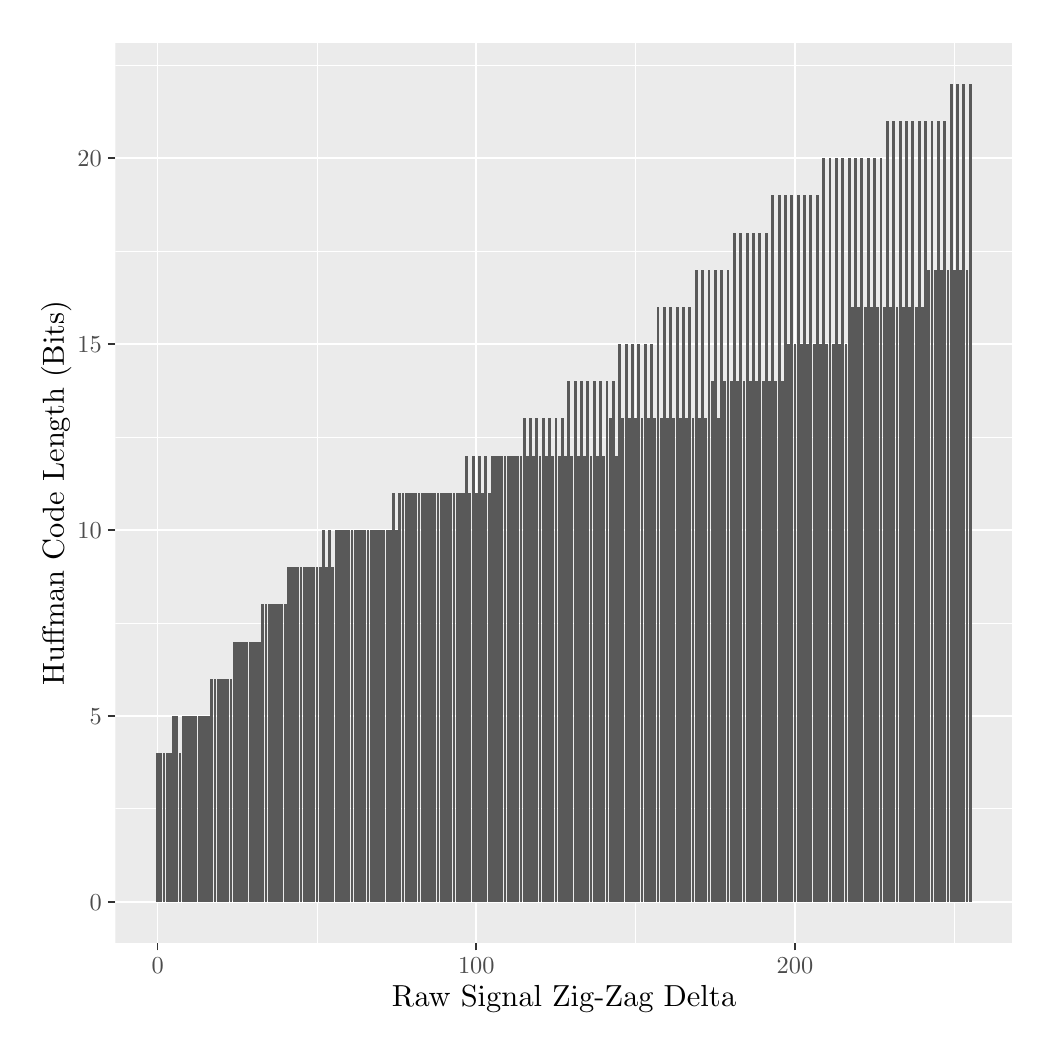
\begin{tikzpicture}[x=1pt,y=1pt]
\definecolor{fillColor}{RGB}{255,255,255}
\path[use as bounding box,fill=fillColor,fill opacity=0.00] (0,0) rectangle (361.35,361.35);
\begin{scope}
\path[clip] (  0.00,  0.00) rectangle (361.35,361.35);
\definecolor{drawColor}{RGB}{255,255,255}
\definecolor{fillColor}{RGB}{255,255,255}

\path[draw=drawColor,line width= 0.6pt,line join=round,line cap=round,fill=fillColor] (  0.00,  0.00) rectangle (361.35,361.35);
\end{scope}
\begin{scope}
\path[clip] ( 31.71, 30.69) rectangle (355.85,355.85);
\definecolor{fillColor}{gray}{0.92}

\path[fill=fillColor] ( 31.71, 30.69) rectangle (355.85,355.85);
\definecolor{drawColor}{RGB}{255,255,255}

\path[draw=drawColor,line width= 0.3pt,line join=round] ( 31.71, 79.06) --
	(355.85, 79.06);

\path[draw=drawColor,line width= 0.3pt,line join=round] ( 31.71,146.24) --
	(355.85,146.24);

\path[draw=drawColor,line width= 0.3pt,line join=round] ( 31.71,213.42) --
	(355.85,213.42);

\path[draw=drawColor,line width= 0.3pt,line join=round] ( 31.71,280.61) --
	(355.85,280.61);

\path[draw=drawColor,line width= 0.3pt,line join=round] ( 31.71,347.79) --
	(355.85,347.79);

\path[draw=drawColor,line width= 0.3pt,line join=round] (104.54, 30.69) --
	(104.54,355.85);

\path[draw=drawColor,line width= 0.3pt,line join=round] (219.69, 30.69) --
	(219.69,355.85);

\path[draw=drawColor,line width= 0.3pt,line join=round] (334.84, 30.69) --
	(334.84,355.85);

\path[draw=drawColor,line width= 0.6pt,line join=round] ( 31.71, 45.47) --
	(355.85, 45.47);

\path[draw=drawColor,line width= 0.6pt,line join=round] ( 31.71,112.65) --
	(355.85,112.65);

\path[draw=drawColor,line width= 0.6pt,line join=round] ( 31.71,179.83) --
	(355.85,179.83);

\path[draw=drawColor,line width= 0.6pt,line join=round] ( 31.71,247.01) --
	(355.85,247.01);

\path[draw=drawColor,line width= 0.6pt,line join=round] ( 31.71,314.20) --
	(355.85,314.20);

\path[draw=drawColor,line width= 0.6pt,line join=round] ( 46.96, 30.69) --
	( 46.96,355.85);

\path[draw=drawColor,line width= 0.6pt,line join=round] (162.11, 30.69) --
	(162.11,355.85);

\path[draw=drawColor,line width= 0.6pt,line join=round] (277.27, 30.69) --
	(277.27,355.85);
\definecolor{fillColor}{gray}{0.35}

\path[fill=fillColor] ( 46.45, 45.47) rectangle ( 47.48, 99.21);

\path[fill=fillColor] ( 47.60, 45.47) rectangle ( 48.63, 99.21);

\path[fill=fillColor] ( 48.75, 45.47) rectangle ( 49.79, 99.21);

\path[fill=fillColor] ( 49.90, 45.47) rectangle ( 50.94, 99.21);

\path[fill=fillColor] ( 51.05, 45.47) rectangle ( 52.09, 99.21);

\path[fill=fillColor] ( 52.20, 45.47) rectangle ( 53.24,112.65);

\path[fill=fillColor] ( 53.35, 45.47) rectangle ( 54.39,112.65);

\path[fill=fillColor] ( 54.51, 45.47) rectangle ( 55.54, 99.21);

\path[fill=fillColor] ( 55.66, 45.47) rectangle ( 56.69,112.65);

\path[fill=fillColor] ( 56.81, 45.47) rectangle ( 57.85,112.65);

\path[fill=fillColor] ( 57.96, 45.47) rectangle ( 59.00,112.65);

\path[fill=fillColor] ( 59.11, 45.47) rectangle ( 60.15,112.65);

\path[fill=fillColor] ( 60.26, 45.47) rectangle ( 61.30,112.65);

\path[fill=fillColor] ( 61.42, 45.47) rectangle ( 62.45,112.65);

\path[fill=fillColor] ( 62.57, 45.47) rectangle ( 63.60,112.65);

\path[fill=fillColor] ( 63.72, 45.47) rectangle ( 64.75,112.65);

\path[fill=fillColor] ( 64.87, 45.47) rectangle ( 65.91,112.65);

\path[fill=fillColor] ( 66.02, 45.47) rectangle ( 67.06,126.09);

\path[fill=fillColor] ( 67.17, 45.47) rectangle ( 68.21,126.09);

\path[fill=fillColor] ( 68.32, 45.47) rectangle ( 69.36,126.09);

\path[fill=fillColor] ( 69.48, 45.47) rectangle ( 70.51,126.09);

\path[fill=fillColor] ( 70.63, 45.47) rectangle ( 71.66,126.09);

\path[fill=fillColor] ( 71.78, 45.47) rectangle ( 72.82,126.09);

\path[fill=fillColor] ( 72.93, 45.47) rectangle ( 73.97,126.09);

\path[fill=fillColor] ( 74.08, 45.47) rectangle ( 75.12,139.52);

\path[fill=fillColor] ( 75.23, 45.47) rectangle ( 76.27,139.52);

\path[fill=fillColor] ( 76.38, 45.47) rectangle ( 77.42,139.52);

\path[fill=fillColor] ( 77.54, 45.47) rectangle ( 78.57,139.52);

\path[fill=fillColor] ( 78.69, 45.47) rectangle ( 79.72,139.52);

\path[fill=fillColor] ( 79.84, 45.47) rectangle ( 80.88,139.52);

\path[fill=fillColor] ( 80.99, 45.47) rectangle ( 82.03,139.52);

\path[fill=fillColor] ( 82.14, 45.47) rectangle ( 83.18,139.52);

\path[fill=fillColor] ( 83.29, 45.47) rectangle ( 84.33,139.52);

\path[fill=fillColor] ( 84.45, 45.47) rectangle ( 85.48,152.96);

\path[fill=fillColor] ( 85.60, 45.47) rectangle ( 86.63,152.96);

\path[fill=fillColor] ( 86.75, 45.47) rectangle ( 87.78,152.96);

\path[fill=fillColor] ( 87.90, 45.47) rectangle ( 88.94,152.96);

\path[fill=fillColor] ( 89.05, 45.47) rectangle ( 90.09,152.96);

\path[fill=fillColor] ( 90.20, 45.47) rectangle ( 91.24,152.96);

\path[fill=fillColor] ( 91.35, 45.47) rectangle ( 92.39,152.96);

\path[fill=fillColor] ( 92.51, 45.47) rectangle ( 93.54,152.96);

\path[fill=fillColor] ( 93.66, 45.47) rectangle ( 94.69,166.39);

\path[fill=fillColor] ( 94.81, 45.47) rectangle ( 95.85,166.39);

\path[fill=fillColor] ( 95.96, 45.47) rectangle ( 97.00,166.39);

\path[fill=fillColor] ( 97.11, 45.47) rectangle ( 98.15,166.39);

\path[fill=fillColor] ( 98.26, 45.47) rectangle ( 99.30,166.39);

\path[fill=fillColor] ( 99.42, 45.47) rectangle (100.45,166.39);

\path[fill=fillColor] (100.57, 45.47) rectangle (101.60,166.39);

\path[fill=fillColor] (101.72, 45.47) rectangle (102.75,166.39);

\path[fill=fillColor] (102.87, 45.47) rectangle (103.91,166.39);

\path[fill=fillColor] (104.02, 45.47) rectangle (105.06,166.39);

\path[fill=fillColor] (105.17, 45.47) rectangle (106.21,166.39);

\path[fill=fillColor] (106.32, 45.47) rectangle (107.36,179.83);

\path[fill=fillColor] (107.48, 45.47) rectangle (108.51,166.39);

\path[fill=fillColor] (108.63, 45.47) rectangle (109.66,179.83);

\path[fill=fillColor] (109.78, 45.47) rectangle (110.82,166.39);

\path[fill=fillColor] (110.93, 45.47) rectangle (111.97,179.83);

\path[fill=fillColor] (112.08, 45.47) rectangle (113.12,179.83);

\path[fill=fillColor] (113.23, 45.47) rectangle (114.27,179.83);

\path[fill=fillColor] (114.38, 45.47) rectangle (115.42,179.83);

\path[fill=fillColor] (115.54, 45.47) rectangle (116.57,179.83);

\path[fill=fillColor] (116.69, 45.47) rectangle (117.72,179.83);

\path[fill=fillColor] (117.84, 45.47) rectangle (118.88,179.83);

\path[fill=fillColor] (118.99, 45.47) rectangle (120.03,179.83);

\path[fill=fillColor] (120.14, 45.47) rectangle (121.18,179.83);

\path[fill=fillColor] (121.29, 45.47) rectangle (122.33,179.83);

\path[fill=fillColor] (122.45, 45.47) rectangle (123.48,179.83);

\path[fill=fillColor] (123.60, 45.47) rectangle (124.63,179.83);

\path[fill=fillColor] (124.75, 45.47) rectangle (125.78,179.83);

\path[fill=fillColor] (125.90, 45.47) rectangle (126.94,179.83);

\path[fill=fillColor] (127.05, 45.47) rectangle (128.09,179.83);

\path[fill=fillColor] (128.20, 45.47) rectangle (129.24,179.83);

\path[fill=fillColor] (129.35, 45.47) rectangle (130.39,179.83);

\path[fill=fillColor] (130.51, 45.47) rectangle (131.54,179.83);

\path[fill=fillColor] (131.66, 45.47) rectangle (132.69,193.27);

\path[fill=fillColor] (132.81, 45.47) rectangle (133.85,179.83);

\path[fill=fillColor] (133.96, 45.47) rectangle (135.00,193.27);

\path[fill=fillColor] (135.11, 45.47) rectangle (136.15,193.27);

\path[fill=fillColor] (136.26, 45.47) rectangle (137.30,193.27);

\path[fill=fillColor] (137.41, 45.47) rectangle (138.45,193.27);

\path[fill=fillColor] (138.57, 45.47) rectangle (139.60,193.27);

\path[fill=fillColor] (139.72, 45.47) rectangle (140.75,193.27);

\path[fill=fillColor] (140.87, 45.47) rectangle (141.91,193.27);

\path[fill=fillColor] (142.02, 45.47) rectangle (143.06,193.27);

\path[fill=fillColor] (143.17, 45.47) rectangle (144.21,193.27);

\path[fill=fillColor] (144.32, 45.47) rectangle (145.36,193.27);

\path[fill=fillColor] (145.48, 45.47) rectangle (146.51,193.27);

\path[fill=fillColor] (146.63, 45.47) rectangle (147.66,193.27);

\path[fill=fillColor] (147.78, 45.47) rectangle (148.81,193.27);

\path[fill=fillColor] (148.93, 45.47) rectangle (149.97,193.27);

\path[fill=fillColor] (150.08, 45.47) rectangle (151.12,193.27);

\path[fill=fillColor] (151.23, 45.47) rectangle (152.27,193.27);

\path[fill=fillColor] (152.38, 45.47) rectangle (153.42,193.27);

\path[fill=fillColor] (153.54, 45.47) rectangle (154.57,193.27);

\path[fill=fillColor] (154.69, 45.47) rectangle (155.72,193.27);

\path[fill=fillColor] (155.84, 45.47) rectangle (156.88,193.27);

\path[fill=fillColor] (156.99, 45.47) rectangle (158.03,193.27);

\path[fill=fillColor] (158.14, 45.47) rectangle (159.18,206.70);

\path[fill=fillColor] (159.29, 45.47) rectangle (160.33,193.27);

\path[fill=fillColor] (160.44, 45.47) rectangle (161.48,206.70);

\path[fill=fillColor] (161.60, 45.47) rectangle (162.63,193.27);

\path[fill=fillColor] (162.75, 45.47) rectangle (163.78,206.70);

\path[fill=fillColor] (163.90, 45.47) rectangle (164.94,193.27);

\path[fill=fillColor] (165.05, 45.47) rectangle (166.09,206.70);

\path[fill=fillColor] (166.20, 45.47) rectangle (167.24,193.27);

\path[fill=fillColor] (167.35, 45.47) rectangle (168.39,206.70);

\path[fill=fillColor] (168.51, 45.47) rectangle (169.54,206.70);

\path[fill=fillColor] (169.66, 45.47) rectangle (170.69,206.70);

\path[fill=fillColor] (170.81, 45.47) rectangle (171.84,206.70);

\path[fill=fillColor] (171.96, 45.47) rectangle (173.00,206.70);

\path[fill=fillColor] (173.11, 45.47) rectangle (174.15,206.70);

\path[fill=fillColor] (174.26, 45.47) rectangle (175.30,206.70);

\path[fill=fillColor] (175.41, 45.47) rectangle (176.45,206.70);

\path[fill=fillColor] (176.57, 45.47) rectangle (177.60,206.70);

\path[fill=fillColor] (177.72, 45.47) rectangle (178.75,206.70);

\path[fill=fillColor] (178.87, 45.47) rectangle (179.91,220.14);

\path[fill=fillColor] (180.02, 45.47) rectangle (181.06,206.70);

\path[fill=fillColor] (181.17, 45.47) rectangle (182.21,220.14);

\path[fill=fillColor] (182.32, 45.47) rectangle (183.36,206.70);

\path[fill=fillColor] (183.48, 45.47) rectangle (184.51,220.14);

\path[fill=fillColor] (184.63, 45.47) rectangle (185.66,206.70);

\path[fill=fillColor] (185.78, 45.47) rectangle (186.81,220.14);

\path[fill=fillColor] (186.93, 45.47) rectangle (187.97,206.70);

\path[fill=fillColor] (188.08, 45.47) rectangle (189.12,220.14);

\path[fill=fillColor] (189.23, 45.47) rectangle (190.27,206.70);

\path[fill=fillColor] (190.38, 45.47) rectangle (191.42,220.14);

\path[fill=fillColor] (191.54, 45.47) rectangle (192.57,206.70);

\path[fill=fillColor] (192.69, 45.47) rectangle (193.72,220.14);

\path[fill=fillColor] (193.84, 45.47) rectangle (194.88,206.70);

\path[fill=fillColor] (194.99, 45.47) rectangle (196.03,233.58);

\path[fill=fillColor] (196.14, 45.47) rectangle (197.18,206.70);

\path[fill=fillColor] (197.29, 45.47) rectangle (198.33,233.58);

\path[fill=fillColor] (198.44, 45.47) rectangle (199.48,206.70);

\path[fill=fillColor] (199.60, 45.47) rectangle (200.63,233.58);

\path[fill=fillColor] (200.75, 45.47) rectangle (201.78,206.70);

\path[fill=fillColor] (201.90, 45.47) rectangle (202.94,233.58);

\path[fill=fillColor] (203.05, 45.47) rectangle (204.09,206.70);

\path[fill=fillColor] (204.20, 45.47) rectangle (205.24,233.58);

\path[fill=fillColor] (205.35, 45.47) rectangle (206.39,206.70);

\path[fill=fillColor] (206.51, 45.47) rectangle (207.54,233.58);

\path[fill=fillColor] (207.66, 45.47) rectangle (208.69,206.70);

\path[fill=fillColor] (208.81, 45.47) rectangle (209.84,233.58);

\path[fill=fillColor] (209.96, 45.47) rectangle (211.00,220.14);

\path[fill=fillColor] (211.11, 45.47) rectangle (212.15,233.58);

\path[fill=fillColor] (212.26, 45.47) rectangle (213.30,206.70);

\path[fill=fillColor] (213.41, 45.47) rectangle (214.45,247.01);

\path[fill=fillColor] (214.57, 45.47) rectangle (215.60,220.14);

\path[fill=fillColor] (215.72, 45.47) rectangle (216.75,247.01);

\path[fill=fillColor] (216.87, 45.47) rectangle (217.91,220.14);

\path[fill=fillColor] (218.02, 45.47) rectangle (219.06,247.01);

\path[fill=fillColor] (219.17, 45.47) rectangle (220.21,220.14);

\path[fill=fillColor] (220.32, 45.47) rectangle (221.36,247.01);

\path[fill=fillColor] (221.47, 45.47) rectangle (222.51,220.14);

\path[fill=fillColor] (222.63, 45.47) rectangle (223.66,247.01);

\path[fill=fillColor] (223.78, 45.47) rectangle (224.81,220.14);

\path[fill=fillColor] (224.93, 45.47) rectangle (225.97,247.01);

\path[fill=fillColor] (226.08, 45.47) rectangle (227.12,220.14);

\path[fill=fillColor] (227.23, 45.47) rectangle (228.27,260.45);

\path[fill=fillColor] (228.38, 45.47) rectangle (229.42,220.14);

\path[fill=fillColor] (229.54, 45.47) rectangle (230.57,260.45);

\path[fill=fillColor] (230.69, 45.47) rectangle (231.72,220.14);

\path[fill=fillColor] (231.84, 45.47) rectangle (232.87,260.45);

\path[fill=fillColor] (232.99, 45.47) rectangle (234.03,220.14);

\path[fill=fillColor] (234.14, 45.47) rectangle (235.18,260.45);

\path[fill=fillColor] (235.29, 45.47) rectangle (236.33,220.14);

\path[fill=fillColor] (236.44, 45.47) rectangle (237.48,260.45);

\path[fill=fillColor] (237.60, 45.47) rectangle (238.63,220.14);

\path[fill=fillColor] (238.75, 45.47) rectangle (239.78,260.45);

\path[fill=fillColor] (239.90, 45.47) rectangle (240.94,220.14);

\path[fill=fillColor] (241.05, 45.47) rectangle (242.09,273.89);

\path[fill=fillColor] (242.20, 45.47) rectangle (243.24,220.14);

\path[fill=fillColor] (243.35, 45.47) rectangle (244.39,273.89);

\path[fill=fillColor] (244.51, 45.47) rectangle (245.54,220.14);

\path[fill=fillColor] (245.66, 45.47) rectangle (246.69,273.89);

\path[fill=fillColor] (246.81, 45.47) rectangle (247.84,233.58);

\path[fill=fillColor] (247.96, 45.47) rectangle (249.00,273.89);

\path[fill=fillColor] (249.11, 45.47) rectangle (250.15,220.14);

\path[fill=fillColor] (250.26, 45.47) rectangle (251.30,273.89);

\path[fill=fillColor] (251.41, 45.47) rectangle (252.45,233.58);

\path[fill=fillColor] (252.57, 45.47) rectangle (253.60,273.89);

\path[fill=fillColor] (253.72, 45.47) rectangle (254.75,233.58);

\path[fill=fillColor] (254.87, 45.47) rectangle (255.90,287.32);

\path[fill=fillColor] (256.02, 45.47) rectangle (257.06,233.58);

\path[fill=fillColor] (257.17, 45.47) rectangle (258.21,287.32);

\path[fill=fillColor] (258.32, 45.47) rectangle (259.36,233.58);

\path[fill=fillColor] (259.47, 45.47) rectangle (260.51,287.32);

\path[fill=fillColor] (260.63, 45.47) rectangle (261.66,233.58);

\path[fill=fillColor] (261.78, 45.47) rectangle (262.81,287.32);

\path[fill=fillColor] (262.93, 45.47) rectangle (263.97,233.58);

\path[fill=fillColor] (264.08, 45.47) rectangle (265.12,287.32);

\path[fill=fillColor] (265.23, 45.47) rectangle (266.27,233.58);

\path[fill=fillColor] (266.38, 45.47) rectangle (267.42,287.32);

\path[fill=fillColor] (267.54, 45.47) rectangle (268.57,233.58);

\path[fill=fillColor] (268.69, 45.47) rectangle (269.72,300.76);

\path[fill=fillColor] (269.84, 45.47) rectangle (270.87,233.58);

\path[fill=fillColor] (270.99, 45.47) rectangle (272.03,300.76);

\path[fill=fillColor] (272.14, 45.47) rectangle (273.18,233.58);

\path[fill=fillColor] (273.29, 45.47) rectangle (274.33,300.76);

\path[fill=fillColor] (274.44, 45.47) rectangle (275.48,247.01);

\path[fill=fillColor] (275.60, 45.47) rectangle (276.63,300.76);

\path[fill=fillColor] (276.75, 45.47) rectangle (277.78,247.01);

\path[fill=fillColor] (277.90, 45.47) rectangle (278.94,300.76);

\path[fill=fillColor] (279.05, 45.47) rectangle (280.09,247.01);

\path[fill=fillColor] (280.20, 45.47) rectangle (281.24,300.76);

\path[fill=fillColor] (281.35, 45.47) rectangle (282.39,247.01);

\path[fill=fillColor] (282.50, 45.47) rectangle (283.54,300.76);

\path[fill=fillColor] (283.66, 45.47) rectangle (284.69,247.01);

\path[fill=fillColor] (284.81, 45.47) rectangle (285.84,300.76);

\path[fill=fillColor] (285.96, 45.47) rectangle (287.00,247.01);

\path[fill=fillColor] (287.11, 45.47) rectangle (288.15,314.20);

\path[fill=fillColor] (288.26, 45.47) rectangle (289.30,247.01);

\path[fill=fillColor] (289.41, 45.47) rectangle (290.45,314.20);

\path[fill=fillColor] (290.57, 45.47) rectangle (291.60,247.01);

\path[fill=fillColor] (291.72, 45.47) rectangle (292.75,314.20);

\path[fill=fillColor] (292.87, 45.47) rectangle (293.90,247.01);

\path[fill=fillColor] (294.02, 45.47) rectangle (295.06,314.20);

\path[fill=fillColor] (295.17, 45.47) rectangle (296.21,247.01);

\path[fill=fillColor] (296.32, 45.47) rectangle (297.36,314.20);

\path[fill=fillColor] (297.47, 45.47) rectangle (298.51,260.45);

\path[fill=fillColor] (298.63, 45.47) rectangle (299.66,314.20);

\path[fill=fillColor] (299.78, 45.47) rectangle (300.81,260.45);

\path[fill=fillColor] (300.93, 45.47) rectangle (301.97,314.20);

\path[fill=fillColor] (302.08, 45.47) rectangle (303.12,260.45);

\path[fill=fillColor] (303.23, 45.47) rectangle (304.27,314.20);

\path[fill=fillColor] (304.38, 45.47) rectangle (305.42,260.45);

\path[fill=fillColor] (305.53, 45.47) rectangle (306.57,314.20);

\path[fill=fillColor] (306.69, 45.47) rectangle (307.72,260.45);

\path[fill=fillColor] (307.84, 45.47) rectangle (308.87,314.20);

\path[fill=fillColor] (308.99, 45.47) rectangle (310.03,260.45);

\path[fill=fillColor] (310.14, 45.47) rectangle (311.18,327.63);

\path[fill=fillColor] (311.29, 45.47) rectangle (312.33,260.45);

\path[fill=fillColor] (312.44, 45.47) rectangle (313.48,327.63);

\path[fill=fillColor] (313.60, 45.47) rectangle (314.63,260.45);

\path[fill=fillColor] (314.75, 45.47) rectangle (315.78,327.63);

\path[fill=fillColor] (315.90, 45.47) rectangle (316.93,260.45);

\path[fill=fillColor] (317.05, 45.47) rectangle (318.09,327.63);

\path[fill=fillColor] (318.20, 45.47) rectangle (319.24,260.45);

\path[fill=fillColor] (319.35, 45.47) rectangle (320.39,327.63);

\path[fill=fillColor] (320.50, 45.47) rectangle (321.54,260.45);

\path[fill=fillColor] (321.66, 45.47) rectangle (322.69,327.63);

\path[fill=fillColor] (322.81, 45.47) rectangle (323.84,260.45);

\path[fill=fillColor] (323.96, 45.47) rectangle (325.00,327.63);

\path[fill=fillColor] (325.11, 45.47) rectangle (326.15,273.89);

\path[fill=fillColor] (326.26, 45.47) rectangle (327.30,327.63);

\path[fill=fillColor] (327.41, 45.47) rectangle (328.45,273.89);

\path[fill=fillColor] (328.57, 45.47) rectangle (329.60,327.63);

\path[fill=fillColor] (329.72, 45.47) rectangle (330.75,273.89);

\path[fill=fillColor] (330.87, 45.47) rectangle (331.90,327.63);

\path[fill=fillColor] (332.02, 45.47) rectangle (333.06,273.89);

\path[fill=fillColor] (333.17, 45.47) rectangle (334.21,341.07);

\path[fill=fillColor] (334.32, 45.47) rectangle (335.36,273.89);

\path[fill=fillColor] (335.47, 45.47) rectangle (336.51,341.07);

\path[fill=fillColor] (336.63, 45.47) rectangle (337.66,273.89);

\path[fill=fillColor] (337.78, 45.47) rectangle (338.81,341.07);

\path[fill=fillColor] (338.93, 45.47) rectangle (339.96,273.89);

\path[fill=fillColor] (340.08, 45.47) rectangle (341.12,341.07);
\end{scope}
\begin{scope}
\path[clip] (  0.00,  0.00) rectangle (361.35,361.35);
\definecolor{drawColor}{gray}{0.30}

\node[text=drawColor,anchor=base east,inner sep=0pt, outer sep=0pt, scale=  0.88] at ( 26.76, 42.44) {0};

\node[text=drawColor,anchor=base east,inner sep=0pt, outer sep=0pt, scale=  0.88] at ( 26.76,109.62) {5};

\node[text=drawColor,anchor=base east,inner sep=0pt, outer sep=0pt, scale=  0.88] at ( 26.76,176.80) {10};

\node[text=drawColor,anchor=base east,inner sep=0pt, outer sep=0pt, scale=  0.88] at ( 26.76,243.98) {15};

\node[text=drawColor,anchor=base east,inner sep=0pt, outer sep=0pt, scale=  0.88] at ( 26.76,311.17) {20};
\end{scope}
\begin{scope}
\path[clip] (  0.00,  0.00) rectangle (361.35,361.35);
\definecolor{drawColor}{gray}{0.20}

\path[draw=drawColor,line width= 0.6pt,line join=round] ( 28.96, 45.47) --
	( 31.71, 45.47);

\path[draw=drawColor,line width= 0.6pt,line join=round] ( 28.96,112.65) --
	( 31.71,112.65);

\path[draw=drawColor,line width= 0.6pt,line join=round] ( 28.96,179.83) --
	( 31.71,179.83);

\path[draw=drawColor,line width= 0.6pt,line join=round] ( 28.96,247.01) --
	( 31.71,247.01);

\path[draw=drawColor,line width= 0.6pt,line join=round] ( 28.96,314.20) --
	( 31.71,314.20);
\end{scope}
\begin{scope}
\path[clip] (  0.00,  0.00) rectangle (361.35,361.35);
\definecolor{drawColor}{gray}{0.20}

\path[draw=drawColor,line width= 0.6pt,line join=round] ( 46.96, 27.94) --
	( 46.96, 30.69);

\path[draw=drawColor,line width= 0.6pt,line join=round] (162.11, 27.94) --
	(162.11, 30.69);

\path[draw=drawColor,line width= 0.6pt,line join=round] (277.27, 27.94) --
	(277.27, 30.69);
\end{scope}
\begin{scope}
\path[clip] (  0.00,  0.00) rectangle (361.35,361.35);
\definecolor{drawColor}{gray}{0.30}

\node[text=drawColor,anchor=base,inner sep=0pt, outer sep=0pt, scale=  0.88] at ( 46.96, 19.68) {0};

\node[text=drawColor,anchor=base,inner sep=0pt, outer sep=0pt, scale=  0.88] at (162.11, 19.68) {100};

\node[text=drawColor,anchor=base,inner sep=0pt, outer sep=0pt, scale=  0.88] at (277.27, 19.68) {200};
\end{scope}
\begin{scope}
\path[clip] (  0.00,  0.00) rectangle (361.35,361.35);
\definecolor{drawColor}{RGB}{0,0,0}

\node[text=drawColor,anchor=base,inner sep=0pt, outer sep=0pt, scale=  1.10] at (193.78,  7.64) {Raw Signal Zig-Zag Delta};
\end{scope}
\begin{scope}
\path[clip] (  0.00,  0.00) rectangle (361.35,361.35);
\definecolor{drawColor}{RGB}{0,0,0}

\node[text=drawColor,rotate= 90.00,anchor=base,inner sep=0pt, outer sep=0pt, scale=  1.10] at ( 13.08,193.27) {Huffman Code Length (Bits)};
\end{scope}
\end{tikzpicture}

	\caption[The Huffman code length of each one-byte zig-zag delta from the shared Huffman table.]{\label{fig:shuff-len}The Huffman code length of each one-byte zig-zag delta from the shared Huffman table, generated using the frequency distribution of the whole data set.}
\end{figure}


\subsection{Range Coding}

Now consider encoding the one-byte data using range coding rather than Huffman
coding. Recall that range coding encodes all of the data into one number given
each symbol's probability of occurrence.  An appropriate initial range of
numbers is chosen. Then, for each symbol in the data stream the current range is
narrowed down based on the current symbol's probability of occurrence. A
representative number from the final range is then chosen as the output.

The probability distribution can be predetermined, calculated by an initial pass
or predicted adaptively. Most available implementations use models
for predicting the probability distribution of the next symbol. These typically
consist of models such as order-0, order-1, order-2 and context mixing which combines
two such algorithms to yield higher accuracy predictions. Secondary symbol
estimation (SSE) is a prediction postprocessing approach which uses the combined
prediction of context mixing and a small context to generate a refined
prediction. The range coding algorithm which applies order-0 and order-1 context
mixing with SSE we'll abbreviate to \textit{rccm01sse}.

The order-$n$ model gives the probability distribution of the next symbol given
the previous $n$ symbols (context). It is updated at each step to increase the
revealed symbol's probability when the same context appears again. For example,
the order-0 model stores the probability distribution of the data up to the
current symbol.

% http://mattmahoney.net/dc/dce.html


% TODO analyse how much better

The compact and regular vbbe21 algorithms still take linear time during encoding
and decoding although require more operations than the naive one byte two byte
exceptions encoding. However, the exceptions section usually accounts for only
36 bytes of the read on average in the vbe21-zd format. Hence, focussing on
compressing the one-byte data section has much more potential benefit.

% TODO compare improvement in results

\subsection{Huffman}

Consider compressing the one-byte data using the Huffman (shortened to
\textit{huff}) coding algorithm. This requires determining the read's zig-zag
delta distribution on an initial pass. Then, the Huffman table is recorded and
each byte is encoded with its Huffman code. The problem is that there is an
overhead with storing the table.  Naively, one can store the table by writing
the number of entries in the table (1 byte) then each entry's symbol (1 byte),
code length (1 byte) and code (code length in bytes). The resulting table
consumes
\[ 1 + 2m + \sum_{i=1}^m\lceil b_i / 8 \rceil \]
bytes where $m\in\mathbb{Z}\cap[0,255]$ is the number of entries in the table
and $b_i$ is the length of the $i$-th entry's code in bits. The number of
entries is the number of unique one-byte zig-zag deltas in the read which is
dependent on the read's length. Short reads may only contain 100 unique one-byte
deltas whilst long reads may easily contain more than 250 entries. If we
estimate that this is roughly 200 and the average code length is 2 bytes then
the table consumes
\[ 1 + 2\times 200 + 200\times 2 = 801 \]
bytes. The maximum number of entries is 256 so the maximum table size is roughly
1025 bytes.

However, rather than encoding the exact Huffman table of each read it makes more
sense to use a shared Huffman table which approximates the zig-zag delta
distribution of most reads well.
%These are bytes we don't need to repeat in each read when each read has a similar distribution of zig-zag deltas.
For example, 0 is the most common value among reads so naturally its code will
have the fewest number of bits and this will be efficient for the majority of
reads. One simple approach is to construct the optimal Huffman table for the
whole data set of zig-zag deltas. Then, we can store the code table once in the
source code and encode each read using the same table. Let's call this method
the static Huffman algorithm or \textit{shuff} for short. This table consumes
1042 bytes but we can store it statically alongside the source code, so unless
we are considering the Kolmogorov complexity of the data its size is not
calculated in the compression size. The distribution of code lengths from this
table is shown in Figure \ref{fig:shuff-len}. The figure shows the distribution
splits into two alternating distributions from about 116 onwards which
represents the higher frequency of large positive compared to large negative
deltas, as previously discussed.

huff consumes more space than the shuff algorithm since it records a different
Huffman table for each read in the compressed data. The space consumed by the
Huffman table turns out to be more than the difference between the globally
approximated and read-optimal Huffman encoding. For example, on the data set
huff applied to vbe21 (hereafter \textit{huff-vbe21}) consumes 36.10 GiB versus
35.85 GiB for shuff-vbe21 which is a difference of $\sim537$ bytes per read.
This results is a compression ratio of 2.927 versus 2.948.
%Moreover, when applied to a different human DNA data set huff-vbe21 consumes

Furthermore, huff takes longer than shuff during compression and decompression.
During compression, huff must do an initial pass of the read to count the data's
frequencies and then construct the Huffman tree and table. During
decompression, huff must read the table and construct the tree before decoding
the data. shuff doesn't need to perform any of these operations since it
pre-calculates the shared table and tree and stores them in static memory.

During compression, calculating the frequencies takes $O(n)$ time. Then,
constructing the tree takes $O(x^2\log x)$ time using the bottom-up construction
% TODO add reference here
algorithm where $0\le x \le 256$ is the number of unique bytes or exceptions
when being applied to vbe21. Constructing the table requires traversing each
branch on the tree which takes $O(x)$ time since there are $2x-1$ nodes in a
Huffman tree. Then, recording the table takes $O(x)$ time and encoding the bytes
takes $O(n)$ time using the table. In total, the huff algorithm takes
$O(n + x^2\log x)$ time for compression while shuff takes $O(n)$ time. Compared
to $n$, the size of the input, $x$ is usually a lot smaller so it has a small
but true effect on the compression time.

During decompression, huff take $O(n + x)$ time since it must construct the tree
whilst shuff takes $O(n)$ time. But in practicality they take the same time. All
in all, as long as there is a benefit to using shuff, which there usually is if
the approximation is good, shuff is faster than huff during compression and
decompression.

\begin{figure}
	\centering
% Created by tikzDevice version 0.12.3.1 on 2022-10-12 14:52:31
% !TEX encoding = UTF-8 Unicode
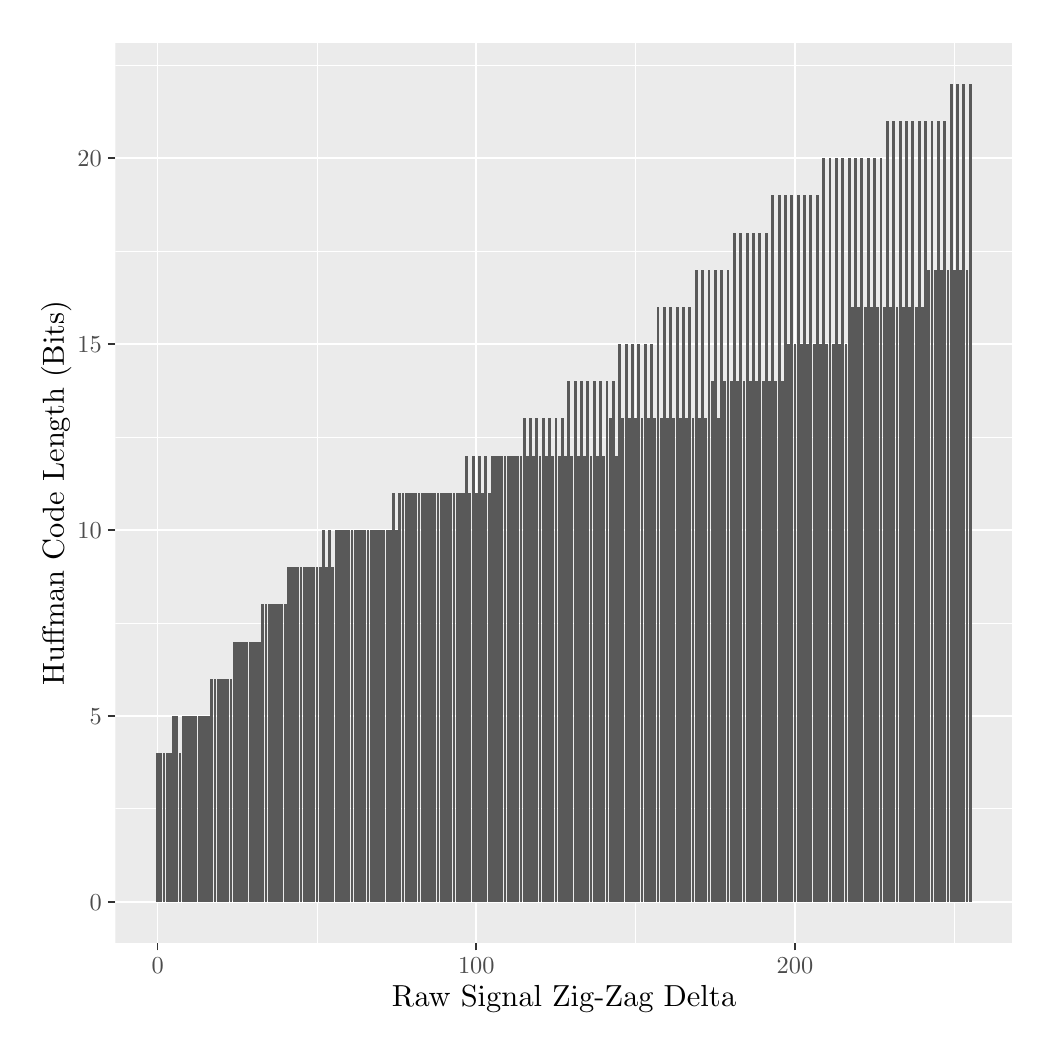
\begin{tikzpicture}[x=1pt,y=1pt]
\definecolor{fillColor}{RGB}{255,255,255}
\path[use as bounding box,fill=fillColor,fill opacity=0.00] (0,0) rectangle (361.35,361.35);
\begin{scope}
\path[clip] (  0.00,  0.00) rectangle (361.35,361.35);
\definecolor{drawColor}{RGB}{255,255,255}
\definecolor{fillColor}{RGB}{255,255,255}

\path[draw=drawColor,line width= 0.6pt,line join=round,line cap=round,fill=fillColor] (  0.00,  0.00) rectangle (361.35,361.35);
\end{scope}
\begin{scope}
\path[clip] ( 31.71, 30.69) rectangle (355.85,355.85);
\definecolor{fillColor}{gray}{0.92}

\path[fill=fillColor] ( 31.71, 30.69) rectangle (355.85,355.85);
\definecolor{drawColor}{RGB}{255,255,255}

\path[draw=drawColor,line width= 0.3pt,line join=round] ( 31.71, 79.06) --
	(355.85, 79.06);

\path[draw=drawColor,line width= 0.3pt,line join=round] ( 31.71,146.24) --
	(355.85,146.24);

\path[draw=drawColor,line width= 0.3pt,line join=round] ( 31.71,213.42) --
	(355.85,213.42);

\path[draw=drawColor,line width= 0.3pt,line join=round] ( 31.71,280.61) --
	(355.85,280.61);

\path[draw=drawColor,line width= 0.3pt,line join=round] ( 31.71,347.79) --
	(355.85,347.79);

\path[draw=drawColor,line width= 0.3pt,line join=round] (104.54, 30.69) --
	(104.54,355.85);

\path[draw=drawColor,line width= 0.3pt,line join=round] (219.69, 30.69) --
	(219.69,355.85);

\path[draw=drawColor,line width= 0.3pt,line join=round] (334.84, 30.69) --
	(334.84,355.85);

\path[draw=drawColor,line width= 0.6pt,line join=round] ( 31.71, 45.47) --
	(355.85, 45.47);

\path[draw=drawColor,line width= 0.6pt,line join=round] ( 31.71,112.65) --
	(355.85,112.65);

\path[draw=drawColor,line width= 0.6pt,line join=round] ( 31.71,179.83) --
	(355.85,179.83);

\path[draw=drawColor,line width= 0.6pt,line join=round] ( 31.71,247.01) --
	(355.85,247.01);

\path[draw=drawColor,line width= 0.6pt,line join=round] ( 31.71,314.20) --
	(355.85,314.20);

\path[draw=drawColor,line width= 0.6pt,line join=round] ( 46.96, 30.69) --
	( 46.96,355.85);

\path[draw=drawColor,line width= 0.6pt,line join=round] (162.11, 30.69) --
	(162.11,355.85);

\path[draw=drawColor,line width= 0.6pt,line join=round] (277.27, 30.69) --
	(277.27,355.85);
\definecolor{fillColor}{gray}{0.35}

\path[fill=fillColor] ( 46.45, 45.47) rectangle ( 47.48, 99.21);

\path[fill=fillColor] ( 47.60, 45.47) rectangle ( 48.63, 99.21);

\path[fill=fillColor] ( 48.75, 45.47) rectangle ( 49.79, 99.21);

\path[fill=fillColor] ( 49.90, 45.47) rectangle ( 50.94, 99.21);

\path[fill=fillColor] ( 51.05, 45.47) rectangle ( 52.09, 99.21);

\path[fill=fillColor] ( 52.20, 45.47) rectangle ( 53.24,112.65);

\path[fill=fillColor] ( 53.35, 45.47) rectangle ( 54.39,112.65);

\path[fill=fillColor] ( 54.51, 45.47) rectangle ( 55.54, 99.21);

\path[fill=fillColor] ( 55.66, 45.47) rectangle ( 56.69,112.65);

\path[fill=fillColor] ( 56.81, 45.47) rectangle ( 57.85,112.65);

\path[fill=fillColor] ( 57.96, 45.47) rectangle ( 59.00,112.65);

\path[fill=fillColor] ( 59.11, 45.47) rectangle ( 60.15,112.65);

\path[fill=fillColor] ( 60.26, 45.47) rectangle ( 61.30,112.65);

\path[fill=fillColor] ( 61.42, 45.47) rectangle ( 62.45,112.65);

\path[fill=fillColor] ( 62.57, 45.47) rectangle ( 63.60,112.65);

\path[fill=fillColor] ( 63.72, 45.47) rectangle ( 64.75,112.65);

\path[fill=fillColor] ( 64.87, 45.47) rectangle ( 65.91,112.65);

\path[fill=fillColor] ( 66.02, 45.47) rectangle ( 67.06,126.09);

\path[fill=fillColor] ( 67.17, 45.47) rectangle ( 68.21,126.09);

\path[fill=fillColor] ( 68.32, 45.47) rectangle ( 69.36,126.09);

\path[fill=fillColor] ( 69.48, 45.47) rectangle ( 70.51,126.09);

\path[fill=fillColor] ( 70.63, 45.47) rectangle ( 71.66,126.09);

\path[fill=fillColor] ( 71.78, 45.47) rectangle ( 72.82,126.09);

\path[fill=fillColor] ( 72.93, 45.47) rectangle ( 73.97,126.09);

\path[fill=fillColor] ( 74.08, 45.47) rectangle ( 75.12,139.52);

\path[fill=fillColor] ( 75.23, 45.47) rectangle ( 76.27,139.52);

\path[fill=fillColor] ( 76.38, 45.47) rectangle ( 77.42,139.52);

\path[fill=fillColor] ( 77.54, 45.47) rectangle ( 78.57,139.52);

\path[fill=fillColor] ( 78.69, 45.47) rectangle ( 79.72,139.52);

\path[fill=fillColor] ( 79.84, 45.47) rectangle ( 80.88,139.52);

\path[fill=fillColor] ( 80.99, 45.47) rectangle ( 82.03,139.52);

\path[fill=fillColor] ( 82.14, 45.47) rectangle ( 83.18,139.52);

\path[fill=fillColor] ( 83.29, 45.47) rectangle ( 84.33,139.52);

\path[fill=fillColor] ( 84.45, 45.47) rectangle ( 85.48,152.96);

\path[fill=fillColor] ( 85.60, 45.47) rectangle ( 86.63,152.96);

\path[fill=fillColor] ( 86.75, 45.47) rectangle ( 87.78,152.96);

\path[fill=fillColor] ( 87.90, 45.47) rectangle ( 88.94,152.96);

\path[fill=fillColor] ( 89.05, 45.47) rectangle ( 90.09,152.96);

\path[fill=fillColor] ( 90.20, 45.47) rectangle ( 91.24,152.96);

\path[fill=fillColor] ( 91.35, 45.47) rectangle ( 92.39,152.96);

\path[fill=fillColor] ( 92.51, 45.47) rectangle ( 93.54,152.96);

\path[fill=fillColor] ( 93.66, 45.47) rectangle ( 94.69,166.39);

\path[fill=fillColor] ( 94.81, 45.47) rectangle ( 95.85,166.39);

\path[fill=fillColor] ( 95.96, 45.47) rectangle ( 97.00,166.39);

\path[fill=fillColor] ( 97.11, 45.47) rectangle ( 98.15,166.39);

\path[fill=fillColor] ( 98.26, 45.47) rectangle ( 99.30,166.39);

\path[fill=fillColor] ( 99.42, 45.47) rectangle (100.45,166.39);

\path[fill=fillColor] (100.57, 45.47) rectangle (101.60,166.39);

\path[fill=fillColor] (101.72, 45.47) rectangle (102.75,166.39);

\path[fill=fillColor] (102.87, 45.47) rectangle (103.91,166.39);

\path[fill=fillColor] (104.02, 45.47) rectangle (105.06,166.39);

\path[fill=fillColor] (105.17, 45.47) rectangle (106.21,166.39);

\path[fill=fillColor] (106.32, 45.47) rectangle (107.36,179.83);

\path[fill=fillColor] (107.48, 45.47) rectangle (108.51,166.39);

\path[fill=fillColor] (108.63, 45.47) rectangle (109.66,179.83);

\path[fill=fillColor] (109.78, 45.47) rectangle (110.82,166.39);

\path[fill=fillColor] (110.93, 45.47) rectangle (111.97,179.83);

\path[fill=fillColor] (112.08, 45.47) rectangle (113.12,179.83);

\path[fill=fillColor] (113.23, 45.47) rectangle (114.27,179.83);

\path[fill=fillColor] (114.38, 45.47) rectangle (115.42,179.83);

\path[fill=fillColor] (115.54, 45.47) rectangle (116.57,179.83);

\path[fill=fillColor] (116.69, 45.47) rectangle (117.72,179.83);

\path[fill=fillColor] (117.84, 45.47) rectangle (118.88,179.83);

\path[fill=fillColor] (118.99, 45.47) rectangle (120.03,179.83);

\path[fill=fillColor] (120.14, 45.47) rectangle (121.18,179.83);

\path[fill=fillColor] (121.29, 45.47) rectangle (122.33,179.83);

\path[fill=fillColor] (122.45, 45.47) rectangle (123.48,179.83);

\path[fill=fillColor] (123.60, 45.47) rectangle (124.63,179.83);

\path[fill=fillColor] (124.75, 45.47) rectangle (125.78,179.83);

\path[fill=fillColor] (125.90, 45.47) rectangle (126.94,179.83);

\path[fill=fillColor] (127.05, 45.47) rectangle (128.09,179.83);

\path[fill=fillColor] (128.20, 45.47) rectangle (129.24,179.83);

\path[fill=fillColor] (129.35, 45.47) rectangle (130.39,179.83);

\path[fill=fillColor] (130.51, 45.47) rectangle (131.54,179.83);

\path[fill=fillColor] (131.66, 45.47) rectangle (132.69,193.27);

\path[fill=fillColor] (132.81, 45.47) rectangle (133.85,179.83);

\path[fill=fillColor] (133.96, 45.47) rectangle (135.00,193.27);

\path[fill=fillColor] (135.11, 45.47) rectangle (136.15,193.27);

\path[fill=fillColor] (136.26, 45.47) rectangle (137.30,193.27);

\path[fill=fillColor] (137.41, 45.47) rectangle (138.45,193.27);

\path[fill=fillColor] (138.57, 45.47) rectangle (139.60,193.27);

\path[fill=fillColor] (139.72, 45.47) rectangle (140.75,193.27);

\path[fill=fillColor] (140.87, 45.47) rectangle (141.91,193.27);

\path[fill=fillColor] (142.02, 45.47) rectangle (143.06,193.27);

\path[fill=fillColor] (143.17, 45.47) rectangle (144.21,193.27);

\path[fill=fillColor] (144.32, 45.47) rectangle (145.36,193.27);

\path[fill=fillColor] (145.48, 45.47) rectangle (146.51,193.27);

\path[fill=fillColor] (146.63, 45.47) rectangle (147.66,193.27);

\path[fill=fillColor] (147.78, 45.47) rectangle (148.81,193.27);

\path[fill=fillColor] (148.93, 45.47) rectangle (149.97,193.27);

\path[fill=fillColor] (150.08, 45.47) rectangle (151.12,193.27);

\path[fill=fillColor] (151.23, 45.47) rectangle (152.27,193.27);

\path[fill=fillColor] (152.38, 45.47) rectangle (153.42,193.27);

\path[fill=fillColor] (153.54, 45.47) rectangle (154.57,193.27);

\path[fill=fillColor] (154.69, 45.47) rectangle (155.72,193.27);

\path[fill=fillColor] (155.84, 45.47) rectangle (156.88,193.27);

\path[fill=fillColor] (156.99, 45.47) rectangle (158.03,193.27);

\path[fill=fillColor] (158.14, 45.47) rectangle (159.18,206.70);

\path[fill=fillColor] (159.29, 45.47) rectangle (160.33,193.27);

\path[fill=fillColor] (160.44, 45.47) rectangle (161.48,206.70);

\path[fill=fillColor] (161.60, 45.47) rectangle (162.63,193.27);

\path[fill=fillColor] (162.75, 45.47) rectangle (163.78,206.70);

\path[fill=fillColor] (163.90, 45.47) rectangle (164.94,193.27);

\path[fill=fillColor] (165.05, 45.47) rectangle (166.09,206.70);

\path[fill=fillColor] (166.20, 45.47) rectangle (167.24,193.27);

\path[fill=fillColor] (167.35, 45.47) rectangle (168.39,206.70);

\path[fill=fillColor] (168.51, 45.47) rectangle (169.54,206.70);

\path[fill=fillColor] (169.66, 45.47) rectangle (170.69,206.70);

\path[fill=fillColor] (170.81, 45.47) rectangle (171.84,206.70);

\path[fill=fillColor] (171.96, 45.47) rectangle (173.00,206.70);

\path[fill=fillColor] (173.11, 45.47) rectangle (174.15,206.70);

\path[fill=fillColor] (174.26, 45.47) rectangle (175.30,206.70);

\path[fill=fillColor] (175.41, 45.47) rectangle (176.45,206.70);

\path[fill=fillColor] (176.57, 45.47) rectangle (177.60,206.70);

\path[fill=fillColor] (177.72, 45.47) rectangle (178.75,206.70);

\path[fill=fillColor] (178.87, 45.47) rectangle (179.91,220.14);

\path[fill=fillColor] (180.02, 45.47) rectangle (181.06,206.70);

\path[fill=fillColor] (181.17, 45.47) rectangle (182.21,220.14);

\path[fill=fillColor] (182.32, 45.47) rectangle (183.36,206.70);

\path[fill=fillColor] (183.48, 45.47) rectangle (184.51,220.14);

\path[fill=fillColor] (184.63, 45.47) rectangle (185.66,206.70);

\path[fill=fillColor] (185.78, 45.47) rectangle (186.81,220.14);

\path[fill=fillColor] (186.93, 45.47) rectangle (187.97,206.70);

\path[fill=fillColor] (188.08, 45.47) rectangle (189.12,220.14);

\path[fill=fillColor] (189.23, 45.47) rectangle (190.27,206.70);

\path[fill=fillColor] (190.38, 45.47) rectangle (191.42,220.14);

\path[fill=fillColor] (191.54, 45.47) rectangle (192.57,206.70);

\path[fill=fillColor] (192.69, 45.47) rectangle (193.72,220.14);

\path[fill=fillColor] (193.84, 45.47) rectangle (194.88,206.70);

\path[fill=fillColor] (194.99, 45.47) rectangle (196.03,233.58);

\path[fill=fillColor] (196.14, 45.47) rectangle (197.18,206.70);

\path[fill=fillColor] (197.29, 45.47) rectangle (198.33,233.58);

\path[fill=fillColor] (198.44, 45.47) rectangle (199.48,206.70);

\path[fill=fillColor] (199.60, 45.47) rectangle (200.63,233.58);

\path[fill=fillColor] (200.75, 45.47) rectangle (201.78,206.70);

\path[fill=fillColor] (201.90, 45.47) rectangle (202.94,233.58);

\path[fill=fillColor] (203.05, 45.47) rectangle (204.09,206.70);

\path[fill=fillColor] (204.20, 45.47) rectangle (205.24,233.58);

\path[fill=fillColor] (205.35, 45.47) rectangle (206.39,206.70);

\path[fill=fillColor] (206.51, 45.47) rectangle (207.54,233.58);

\path[fill=fillColor] (207.66, 45.47) rectangle (208.69,206.70);

\path[fill=fillColor] (208.81, 45.47) rectangle (209.84,233.58);

\path[fill=fillColor] (209.96, 45.47) rectangle (211.00,220.14);

\path[fill=fillColor] (211.11, 45.47) rectangle (212.15,233.58);

\path[fill=fillColor] (212.26, 45.47) rectangle (213.30,206.70);

\path[fill=fillColor] (213.41, 45.47) rectangle (214.45,247.01);

\path[fill=fillColor] (214.57, 45.47) rectangle (215.60,220.14);

\path[fill=fillColor] (215.72, 45.47) rectangle (216.75,247.01);

\path[fill=fillColor] (216.87, 45.47) rectangle (217.91,220.14);

\path[fill=fillColor] (218.02, 45.47) rectangle (219.06,247.01);

\path[fill=fillColor] (219.17, 45.47) rectangle (220.21,220.14);

\path[fill=fillColor] (220.32, 45.47) rectangle (221.36,247.01);

\path[fill=fillColor] (221.47, 45.47) rectangle (222.51,220.14);

\path[fill=fillColor] (222.63, 45.47) rectangle (223.66,247.01);

\path[fill=fillColor] (223.78, 45.47) rectangle (224.81,220.14);

\path[fill=fillColor] (224.93, 45.47) rectangle (225.97,247.01);

\path[fill=fillColor] (226.08, 45.47) rectangle (227.12,220.14);

\path[fill=fillColor] (227.23, 45.47) rectangle (228.27,260.45);

\path[fill=fillColor] (228.38, 45.47) rectangle (229.42,220.14);

\path[fill=fillColor] (229.54, 45.47) rectangle (230.57,260.45);

\path[fill=fillColor] (230.69, 45.47) rectangle (231.72,220.14);

\path[fill=fillColor] (231.84, 45.47) rectangle (232.87,260.45);

\path[fill=fillColor] (232.99, 45.47) rectangle (234.03,220.14);

\path[fill=fillColor] (234.14, 45.47) rectangle (235.18,260.45);

\path[fill=fillColor] (235.29, 45.47) rectangle (236.33,220.14);

\path[fill=fillColor] (236.44, 45.47) rectangle (237.48,260.45);

\path[fill=fillColor] (237.60, 45.47) rectangle (238.63,220.14);

\path[fill=fillColor] (238.75, 45.47) rectangle (239.78,260.45);

\path[fill=fillColor] (239.90, 45.47) rectangle (240.94,220.14);

\path[fill=fillColor] (241.05, 45.47) rectangle (242.09,273.89);

\path[fill=fillColor] (242.20, 45.47) rectangle (243.24,220.14);

\path[fill=fillColor] (243.35, 45.47) rectangle (244.39,273.89);

\path[fill=fillColor] (244.51, 45.47) rectangle (245.54,220.14);

\path[fill=fillColor] (245.66, 45.47) rectangle (246.69,273.89);

\path[fill=fillColor] (246.81, 45.47) rectangle (247.84,233.58);

\path[fill=fillColor] (247.96, 45.47) rectangle (249.00,273.89);

\path[fill=fillColor] (249.11, 45.47) rectangle (250.15,220.14);

\path[fill=fillColor] (250.26, 45.47) rectangle (251.30,273.89);

\path[fill=fillColor] (251.41, 45.47) rectangle (252.45,233.58);

\path[fill=fillColor] (252.57, 45.47) rectangle (253.60,273.89);

\path[fill=fillColor] (253.72, 45.47) rectangle (254.75,233.58);

\path[fill=fillColor] (254.87, 45.47) rectangle (255.90,287.32);

\path[fill=fillColor] (256.02, 45.47) rectangle (257.06,233.58);

\path[fill=fillColor] (257.17, 45.47) rectangle (258.21,287.32);

\path[fill=fillColor] (258.32, 45.47) rectangle (259.36,233.58);

\path[fill=fillColor] (259.47, 45.47) rectangle (260.51,287.32);

\path[fill=fillColor] (260.63, 45.47) rectangle (261.66,233.58);

\path[fill=fillColor] (261.78, 45.47) rectangle (262.81,287.32);

\path[fill=fillColor] (262.93, 45.47) rectangle (263.97,233.58);

\path[fill=fillColor] (264.08, 45.47) rectangle (265.12,287.32);

\path[fill=fillColor] (265.23, 45.47) rectangle (266.27,233.58);

\path[fill=fillColor] (266.38, 45.47) rectangle (267.42,287.32);

\path[fill=fillColor] (267.54, 45.47) rectangle (268.57,233.58);

\path[fill=fillColor] (268.69, 45.47) rectangle (269.72,300.76);

\path[fill=fillColor] (269.84, 45.47) rectangle (270.87,233.58);

\path[fill=fillColor] (270.99, 45.47) rectangle (272.03,300.76);

\path[fill=fillColor] (272.14, 45.47) rectangle (273.18,233.58);

\path[fill=fillColor] (273.29, 45.47) rectangle (274.33,300.76);

\path[fill=fillColor] (274.44, 45.47) rectangle (275.48,247.01);

\path[fill=fillColor] (275.60, 45.47) rectangle (276.63,300.76);

\path[fill=fillColor] (276.75, 45.47) rectangle (277.78,247.01);

\path[fill=fillColor] (277.90, 45.47) rectangle (278.94,300.76);

\path[fill=fillColor] (279.05, 45.47) rectangle (280.09,247.01);

\path[fill=fillColor] (280.20, 45.47) rectangle (281.24,300.76);

\path[fill=fillColor] (281.35, 45.47) rectangle (282.39,247.01);

\path[fill=fillColor] (282.50, 45.47) rectangle (283.54,300.76);

\path[fill=fillColor] (283.66, 45.47) rectangle (284.69,247.01);

\path[fill=fillColor] (284.81, 45.47) rectangle (285.84,300.76);

\path[fill=fillColor] (285.96, 45.47) rectangle (287.00,247.01);

\path[fill=fillColor] (287.11, 45.47) rectangle (288.15,314.20);

\path[fill=fillColor] (288.26, 45.47) rectangle (289.30,247.01);

\path[fill=fillColor] (289.41, 45.47) rectangle (290.45,314.20);

\path[fill=fillColor] (290.57, 45.47) rectangle (291.60,247.01);

\path[fill=fillColor] (291.72, 45.47) rectangle (292.75,314.20);

\path[fill=fillColor] (292.87, 45.47) rectangle (293.90,247.01);

\path[fill=fillColor] (294.02, 45.47) rectangle (295.06,314.20);

\path[fill=fillColor] (295.17, 45.47) rectangle (296.21,247.01);

\path[fill=fillColor] (296.32, 45.47) rectangle (297.36,314.20);

\path[fill=fillColor] (297.47, 45.47) rectangle (298.51,260.45);

\path[fill=fillColor] (298.63, 45.47) rectangle (299.66,314.20);

\path[fill=fillColor] (299.78, 45.47) rectangle (300.81,260.45);

\path[fill=fillColor] (300.93, 45.47) rectangle (301.97,314.20);

\path[fill=fillColor] (302.08, 45.47) rectangle (303.12,260.45);

\path[fill=fillColor] (303.23, 45.47) rectangle (304.27,314.20);

\path[fill=fillColor] (304.38, 45.47) rectangle (305.42,260.45);

\path[fill=fillColor] (305.53, 45.47) rectangle (306.57,314.20);

\path[fill=fillColor] (306.69, 45.47) rectangle (307.72,260.45);

\path[fill=fillColor] (307.84, 45.47) rectangle (308.87,314.20);

\path[fill=fillColor] (308.99, 45.47) rectangle (310.03,260.45);

\path[fill=fillColor] (310.14, 45.47) rectangle (311.18,327.63);

\path[fill=fillColor] (311.29, 45.47) rectangle (312.33,260.45);

\path[fill=fillColor] (312.44, 45.47) rectangle (313.48,327.63);

\path[fill=fillColor] (313.60, 45.47) rectangle (314.63,260.45);

\path[fill=fillColor] (314.75, 45.47) rectangle (315.78,327.63);

\path[fill=fillColor] (315.90, 45.47) rectangle (316.93,260.45);

\path[fill=fillColor] (317.05, 45.47) rectangle (318.09,327.63);

\path[fill=fillColor] (318.20, 45.47) rectangle (319.24,260.45);

\path[fill=fillColor] (319.35, 45.47) rectangle (320.39,327.63);

\path[fill=fillColor] (320.50, 45.47) rectangle (321.54,260.45);

\path[fill=fillColor] (321.66, 45.47) rectangle (322.69,327.63);

\path[fill=fillColor] (322.81, 45.47) rectangle (323.84,260.45);

\path[fill=fillColor] (323.96, 45.47) rectangle (325.00,327.63);

\path[fill=fillColor] (325.11, 45.47) rectangle (326.15,273.89);

\path[fill=fillColor] (326.26, 45.47) rectangle (327.30,327.63);

\path[fill=fillColor] (327.41, 45.47) rectangle (328.45,273.89);

\path[fill=fillColor] (328.57, 45.47) rectangle (329.60,327.63);

\path[fill=fillColor] (329.72, 45.47) rectangle (330.75,273.89);

\path[fill=fillColor] (330.87, 45.47) rectangle (331.90,327.63);

\path[fill=fillColor] (332.02, 45.47) rectangle (333.06,273.89);

\path[fill=fillColor] (333.17, 45.47) rectangle (334.21,341.07);

\path[fill=fillColor] (334.32, 45.47) rectangle (335.36,273.89);

\path[fill=fillColor] (335.47, 45.47) rectangle (336.51,341.07);

\path[fill=fillColor] (336.63, 45.47) rectangle (337.66,273.89);

\path[fill=fillColor] (337.78, 45.47) rectangle (338.81,341.07);

\path[fill=fillColor] (338.93, 45.47) rectangle (339.96,273.89);

\path[fill=fillColor] (340.08, 45.47) rectangle (341.12,341.07);
\end{scope}
\begin{scope}
\path[clip] (  0.00,  0.00) rectangle (361.35,361.35);
\definecolor{drawColor}{gray}{0.30}

\node[text=drawColor,anchor=base east,inner sep=0pt, outer sep=0pt, scale=  0.88] at ( 26.76, 42.44) {0};

\node[text=drawColor,anchor=base east,inner sep=0pt, outer sep=0pt, scale=  0.88] at ( 26.76,109.62) {5};

\node[text=drawColor,anchor=base east,inner sep=0pt, outer sep=0pt, scale=  0.88] at ( 26.76,176.80) {10};

\node[text=drawColor,anchor=base east,inner sep=0pt, outer sep=0pt, scale=  0.88] at ( 26.76,243.98) {15};

\node[text=drawColor,anchor=base east,inner sep=0pt, outer sep=0pt, scale=  0.88] at ( 26.76,311.17) {20};
\end{scope}
\begin{scope}
\path[clip] (  0.00,  0.00) rectangle (361.35,361.35);
\definecolor{drawColor}{gray}{0.20}

\path[draw=drawColor,line width= 0.6pt,line join=round] ( 28.96, 45.47) --
	( 31.71, 45.47);

\path[draw=drawColor,line width= 0.6pt,line join=round] ( 28.96,112.65) --
	( 31.71,112.65);

\path[draw=drawColor,line width= 0.6pt,line join=round] ( 28.96,179.83) --
	( 31.71,179.83);

\path[draw=drawColor,line width= 0.6pt,line join=round] ( 28.96,247.01) --
	( 31.71,247.01);

\path[draw=drawColor,line width= 0.6pt,line join=round] ( 28.96,314.20) --
	( 31.71,314.20);
\end{scope}
\begin{scope}
\path[clip] (  0.00,  0.00) rectangle (361.35,361.35);
\definecolor{drawColor}{gray}{0.20}

\path[draw=drawColor,line width= 0.6pt,line join=round] ( 46.96, 27.94) --
	( 46.96, 30.69);

\path[draw=drawColor,line width= 0.6pt,line join=round] (162.11, 27.94) --
	(162.11, 30.69);

\path[draw=drawColor,line width= 0.6pt,line join=round] (277.27, 27.94) --
	(277.27, 30.69);
\end{scope}
\begin{scope}
\path[clip] (  0.00,  0.00) rectangle (361.35,361.35);
\definecolor{drawColor}{gray}{0.30}

\node[text=drawColor,anchor=base,inner sep=0pt, outer sep=0pt, scale=  0.88] at ( 46.96, 19.68) {0};

\node[text=drawColor,anchor=base,inner sep=0pt, outer sep=0pt, scale=  0.88] at (162.11, 19.68) {100};

\node[text=drawColor,anchor=base,inner sep=0pt, outer sep=0pt, scale=  0.88] at (277.27, 19.68) {200};
\end{scope}
\begin{scope}
\path[clip] (  0.00,  0.00) rectangle (361.35,361.35);
\definecolor{drawColor}{RGB}{0,0,0}

\node[text=drawColor,anchor=base,inner sep=0pt, outer sep=0pt, scale=  1.10] at (193.78,  7.64) {Raw Signal Zig-Zag Delta};
\end{scope}
\begin{scope}
\path[clip] (  0.00,  0.00) rectangle (361.35,361.35);
\definecolor{drawColor}{RGB}{0,0,0}

\node[text=drawColor,rotate= 90.00,anchor=base,inner sep=0pt, outer sep=0pt, scale=  1.10] at ( 13.08,193.27) {Huffman Code Length (Bits)};
\end{scope}
\end{tikzpicture}

	\caption[The Huffman code length of each one-byte zig-zag delta from the shared Huffman table.]{\label{fig:shuff-len}The Huffman code length of each one-byte zig-zag delta from the shared Huffman table, generated using the frequency distribution of the whole data set.}
\end{figure}


\subsection{Range Coding}

Now consider encoding the one-byte data using range coding rather than Huffman
coding. Recall that range coding encodes all of the data into one number given
each symbol's probability of occurrence.  An appropriate initial range of
numbers is chosen. Then, for each symbol in the data stream the current range is
narrowed down based on the current symbol's probability of occurrence. A
representative number from the final range is then chosen as the output.

The probability distribution can be predetermined, calculated by an initial pass
or predicted adaptively. Most available implementations use models
for predicting the probability distribution of the next symbol. These typically
consist of models such as order-0, order-1, order-2 and context mixing which combines
two such algorithms to yield higher accuracy predictions. Secondary symbol
estimation (SSE) is a prediction postprocessing approach which uses the combined
prediction of context mixing and a small context to generate a refined
prediction. The range coding algorithm which applies order-0 and order-1 context
mixing with SSE we'll abbreviate to \textit{rccm01sse}.

The order-$n$ model gives the probability distribution of the next symbol given
the previous $n$ symbols (context). It is updated at each step to increase the
revealed symbol's probability when the same context appears again. For example,
the order-0 model stores the probability distribution of the data up to the
current symbol.

% http://mattmahoney.net/dc/dce.html
